\documentclass[10pt]{article}  

%%%%%%%% PREÁMBULO %%%%%%%%%%%%
\title{Trabajo Terminal I}
\usepackage[spanish]{babel} %Indica que escribiermos en español
\usepackage[utf8]{inputenc} %Indica qué codificación se está usando ISO-8859-1(latin1)  o utf8  
\usepackage{longtable}
\usepackage{amsmath} % Comandos extras para matemáticas (cajas para ecuaciones,
% etc)
\usepackage{amssymb} % Simbolos matematicos (por lo tanto)
\usepackage{graphicx} % Incluir imágenes en LaTeX
\usepackage{eso-pic} 
\usepackage{color} % Para colorear texto
\usepackage{subfigure} % subfiguras
\usepackage{float} %Podemos usar el especificador [H] en las figuras para que se
% queden donde queramos
\usepackage{multirow}
\usepackage{capt-of} % Permite usar etiquetas fuera de elementos flotantes
% (etiquetas de figuras)
\usepackage{sidecap} % Para poner el texto de las imágenes al lado
	\sidecaptionvpos{figure}{c} % Para que el texto se alinie al centro vertical
\usepackage{caption} % Para poder quitar numeracion de figuras
\usepackage{commath} % funcionalidades extras para diferenciales, integrales,
% etc (\od, \dif, etc)
\usepackage{cancel} % para cancelar expresiones (\cancelto{0}{x})
 
\usepackage{anysize} 					% Para personalizar el ancho de  los márgenes
\marginsize{3cm}{2cm}{2cm}{2cm} % Izquierda, derecha, arriba, abajo

\usepackage{appendix}
\renewcommand{\appendixname}{Apéndices}
\renewcommand{\appendixtocname}{Apéndices}
\renewcommand{\appendixpagename}{Apéndices} 

% Para que las referencias sean hipervínculos a las figuras o ecuaciones y
% aparezcan en color
\usepackage[colorlinks=true,plainpages=true,citecolor=blue,linkcolor=blue]{hyperref}
%\usepackage{hyperref} 
% Para agregar encabezado y pie de página


\usepackage{listings} % Para usar código fuente
\definecolor{dkgreen}{rgb}{0,0.6,0} % Definimos colores para usar en el código
\definecolor{gray}{rgb}{0.5,0.5,0.5} 
% configuración para el lenguaje que queramos utilizar
\lstset{language=Matlab,
   keywords={break,case,catch,continue,else,elseif,end,for,function,
      global,if,otherwise,persistent,return,switch,try,while},
   basicstyle=\ttfamily,
   keywordstyle=\color{blue},
   commentstyle=\color{red},
   stringstyle=\color{dkgreen},
   numbers=left,
   numberstyle=\tiny\color{gray},
   stepnumber=1,
   numbersep=10pt,
   backgroundcolor=\color{white},
   tabsize=4,
   showspaces=false,
   showstringspaces=false}

\newcommand{\sen}{\operatorname{\sen}}	% Definimos el comando \sen para el seno
%en español

\title{Trabajo Terminal }

%%%%%%%% TERMINA PREÁMBULO %%%%%%%%%%%%

\begin{document}


%%%%%%%%%%%%%%%%%%%%%%%%%%%%%%%%%% PORTADA %%%%%%%%%%%%%%%%%%%%%%%%%%%%%%%%%%%%%%%%%%%%
																					%%%
\begin{center}																		%%%
\newcommand{\HRule}{\rule{\linewidth}{0.5mm}}									%%%\left
 																					%%%

\begin{figure}[t]
\raggedright

\includegraphics[scale = 0.24]{Imagenes/IPN}
\end{figure}

												%%%
\vspace*{-1.5 cm}								%%%
																					%%%	
\textsc{\LARGE \bfseries INSTITUTO POLITÉCNICO NACIONAL }\\[0.5cm]	\textsc{\large \bfseries ESCUELA SUPERIOR DE CÓMPUTO}\\[1.5cm]
													%%%


\begin{minipage}{0.9\textwidth} 
\begin{center}																					%%%
\textsc{\Large \bfseries ESCOM}
\end{center}
\end{minipage}\\[1.5cm]

\textsc{\large \itshape Trabajo Terminal}\\[0.4cm]

{ \huge \bfseries Prototipo de herramienta de apoyo al daltonismo}\\[0.4cm]	%%%-

{ \large  2019-A094}\\[1.00cm] 																					%%%
													%%%
 																				%%%
																	

\begin{center}
\textsc{\Large \itshape Presenta:}\\[0.4cm]
\end{center}

\textsc{\Large \bfseries Jorge Armando Solis Solis }\\[2.00cm]
								

\begin{center}
\textsc{\Large \itshape Directores:}\\[0.4cm]
\end{center}

\textsc{\Large \bfseries
M. en C. Rafael Norman Saucedo Delgado \\
L.E. Rosa Itzel Solis Solis  }\\[2.00cm]

\end{center}							 											

\begin{minipage}{1.00\textwidth} \begin{flushright}
\textsc{\normalsize \today}\\[0.4cm]
\end{flushright}\end{minipage}


\begin{figure}[b]
\raggedright

\includegraphics[scale = 0.25]{Imagenes/logo.png}
\end{figure}

																				
\newpage																		
%%%%%%%%%%%%%%%%%%%% TERMINA PORTADA %%%%%%%%%%%%%%%%%%%%%%%%%%%%%%%%

\section{Abstract.}
The next Trabajo Terminal propose the creation of a prototype that helps people that suffers differents daltonism types except of achromatopsia. Research is currently needed and in Mexico, the systems are lacking that help to the daltonism people, being only international companies that work in this regard. The contribution will be the detection and correction only while using proposed prototype, having a positive impact on the medical and social problems detected (Discrimination). This will be done using the SCRUM methodology within one year of work, in conjunction with artificial intelligence, through classification algorithms, and Ishihara charts. With the above described, the alteration can be diagnosed in the patient, and in those who are diagnosed correctly distinguish the spectrum of colors in their daily lives.

\newpage
 
\section{Agradecimientos}

Se agradece por su apoyo a las siguientes personas: \\
 Mis padres Rosalba Solis Calderon, Armando Solis Hernández por el gran apoyo que me han dado durante todos los años de mi trayectoria escolar.\\
 
A mis directora y hermana  Rosa Itzel Solis Solis por el apoyo durante todo el Trabajo Terminal, recordando un poco a que durante toda mi carrera he contado con su apoyo incondicional.\\

A mi Director, profesor y amigo. Rafael Norman Saucedo Delgado por no tan solo el haber aceptado ser mi director, si no por el apoyo que me ha brindado en la ayuda en las materias y la cercanía que hemos creado gracias al club de cultura e idioma japonés. \\
Y por su apoyo con las instalaciones para realización de pruebas a mi líder y amigo del partido Mario Becerril Martínez y a su madre y consejal de la G.A.M. María de Jesus Martínez Bravo.

\newpage

\tableofcontents 
\newpage
\listoffigures
\newpage
\listoftables

\newpage


 
\section{Resumen.}

 El siguiente trabajo terminal propone la creación de un prototipo que cuenta con la finalidad de apoyar a la gente que padece diferentes tipos de daltonismo exceptuando la acromatopsia. Actualmente hace falta investigación al respecto y en México se carece de sistemas que apoyen a personas daltónicas, siendo solamente empresas internacionales las que trabajan al respecto. El aporte será el apoyo a su detección y corrección sólo durante el uso del prototipo propuesto, teniendo una repercusión positiva en la problemática médica y social detectada (Discriminación). Esto se realizará utilizando la metodología SCRUM en el lapso de uno año de trabajo, en conjunto con la inteligencia artificial, por medio de algoritmos de clasificación, y las cartas de Ishihara. Con lo anterior descrito, se podrá diagnosticar la alteración en el paciente, y en aquellos que se encuentren diagnosticados el distinguir correctamente el espectro de colores en sus vidas cotidianas.


\section{Objetivo.}

Desarrollar un prototipo de herramienta de apoyo capaz de diagnosticar y mostrar la correcta gama de colores durante su uso  a pacientes con los diferentes tipos de daltonismo, exceptuando la acromatopsia. 

\subsection{Objetivos Específicos.}
\begin{itemize}
\item Diagnosticar pacientes con daltonismo, de manera más práctica a través de la Inteligencia Artificial.
 \item Identificar con mayor facilidad diferentes tipos de daltonismo.
\item Mostrar al paciente el correcto espectro de colores, utilizando la transformación de colores RGB.
\end{itemize}

%\cite{IEEEreferencias:Ref1}

\newpage

\section{Introducción}
John Dalton (1766-1844) fue quien descubrió el daltonismo. Cuando fue a conocer al rey Guillermo IV acudió con un traje académico escarlata (rojo), un color demasiado llamativo para un acto tan solemne. La razón es simple: él veía su ropa de color gris oscuro \cite{IEEEreferencias:Ref1}.


\setlength{\parskip}{2mm}

John Dalton proporcionó una descripción científica sobre este fenómeno que posteriormente se conoció con el nombre de daltonismo. Su último experimento demostró que el daltonismo no es un problema del ojo mismo, sino que estaba causado por alguna deficiencia del poder sensorial \cite{IEEEreferencias:Ref1}.


\setlength{\parskip}{2mm}

La forma más frecuente del daltonismo es que el paciente presente dificultades para distinguir entre el verde (deutaconos) y el rojo (protaconos), aunque puede ocurrir con las tonalidades azules (tritaconos). En cambio, un daltónico puede apreciar más matices del violeta que un sujeto con visión normal[1][2]. Este defecto es genético, aunque también puede adquirirse por una enfermedad ocular o sistémica, e incluso por un traumatismo o uso de algún medicamento \cite{IEEEreferencias:Ref3}.


\setlength{\parskip}{2mm}

Esta ceguera hacia el rojo y el verde afecta a un ocho por ciento de la población masculina de todo el mundo. En América Latina uno de cada doce hombres es daltónico. La mayoría de los casos de daltonismo se deben a un problema genético ligado al sexo. Muy pocas mujeres son daltónicas y aproximadamente uno de cada diez hombres sufren alguna forma de daltonismo \cite{IEEEreferencias:Ref3}.


\setlength{\parskip}{2mm}

Los objetos absorben y reflejan la luz de forma distinta dependiendo de sus características físicas, como su forma, composición, etc. El color que se percibe de un objeto es el rayo de luz que rechaza. Las personas captan esos “rebotes” con diferentes longitudes de onda, gracias a la estructura de los ojos. Si los rayos de luz atraviesan al objeto, éste es invisible. Las células sensoriales (fotorreceptores) de la retina que reaccionan en respuesta a la luz son de dos tipos: conos y bastones. Los bastones se activan en la oscuridad y sólo permiten distinguir el negro, el blanco y los distintos grises. Nos permiten percibir el contraste. Los conos, en cambio, funcionan de día y en ambientes iluminados y hacen posible la visión de los colores. Tanto los conos como los bastones se conectan con los centros cerebrales de la visión por medio del nervio óptico \cite{IEEEreferencias:Ref3}.


\setlength{\parskip}{2mm}

La forma más grave de daltonismo es la acromatopsia. La persona que padece esta rara afección no puede ver ningún color, así que todo lo ve en sombras de gris. La acromatopsia suele estar asociada con ojo perezoso, nistagmos (pequeños movimientos espasmódicos del ojo), fotosensibilidad grave y extremadamente mala visión. Su diagnóstico es llevado a cabo por un oftalmólogo y dos principales herramientas como lo son las cartas de Ishihara y/o el test de Farnsworth\cite{IEEEreferencias:Ref3}.

\setlength{\parskip}{2mm}

En la actualidad no se cuenta con tratamiento para el daltonismo, sólo con distintos dispositivos de apoyo \cite{IEEEreferencias:Ref1}. Sin embargo, se podría estar cerca de conseguir una cura para el daltonismo, el profesor Jay Neitz y su equipo consiguieron su objetivo introduciendo genes terapéuticos en las células de la parte trasera del ojo de un mono adulto macho. Esos genes contenían el código de A.D.N. (Ácido Desoxiribo Nucléico) necesario para distinguir los colores. La terapia resultó ser todo un éxito, ya que tras la intervención los monos tratados pudieron señalar correctamente las formas rojas que aparecían en fondos verdes, así lograron restaurar la visión de todos los colores en monos adultos que nacieron sin la habilidad de distinguir entre el rojo y el verde. Los expertos aseguran que el mismo tratamiento podría funcionar en humanos\cite{IEEEreferencias:Ref4}.
\newpage
\section{Antecedentes}
\subsection{Daltonismo}
El daltonismo está enmarcado en la discromatopsia, un término que hace referencia a un inconveniente basado en la incapacidad para diferenciar los colores, debido a la falta de funcionamiento de las células encargadas de su percepción. Es más frecuente de lo pensado, más habitual en los varones y en la mayoría de los casos se trata de un problema genético \cite{IEEEreferencias:Ref1}\cite{IEEEreferencias:Ref2}.

\setlength{\parskip}{2mm}

Quien descubrió este defecto fue el naturalista, químico y matemático de origen inglés John Dalton (1766-1844).
Cuentan que cuando fue a conocer al rey Guillermo IV acudió con un traje académico escarlata (rojo), un color demasiado llamativo para un acto tan solemne. La razón es simple: él veía su ropa de color gris oscuro \cite{IEEEreferencias:Ref1}.

\subsection{John Dalton}

A la edad de 26 años (1792), Dalton descubrió que ni él ni su hermano eran capaces de distinguir los colores. Le regaló a su madre unas medias (que él creía azules) y ella le preguntó sorprendida cuál era la razón por la que le daba unas medias de color escarlata, que no era apropiado para una mujer cuáquera. En su primer artículo científico importante, John Dalton proporcionó una descripción científica sobre este fenómeno que posteriormente se conoció con el nombre de daltonismo \cite{IEEEreferencias:Ref1}.

\setlength{\parskip}{2mm}

Así describía su discapacidad en \textit{<<Memoirs of the Manchester Literary and Philosophical Society>>}:

\textit{<<Siempre fui de la opinión, aunque no soliera mencionarla, de que los nombres de algunos colores eran muy poco razonables. El término rosa, en referencia a la flor de dicho nombre, parecía bastante adecuado; pero cuando se utilizaba el término rojo en lugar de rosa lo consideraba muy inadecuado; para mí debería haber sido azul, pues rosa y azul me parecían muy estrechamente relacionados [el rosa en cuestión debía haber sido más próximo al malva, ya que Dalton habría sido insensible al componente rojo]; mientras que rosa y rojo apenas tienen cualquier relación. }.

\setlength{\parskip}{2mm}

\textit{En el curso de mi dedicación a las ciencias, la de la óptica reclamaba necesariamente atención y me familiaricé muy bien con la teoría de la luz y los colores antes de que apreciara ninguna peculiaridad en mi visión. Sin embargo, yo no había prestado mucho interés a la discriminación práctica de los colores debido, en cierto modo, a lo que yo imaginaba que era una extrañeza de su nomenclatura. A partir del año 1.790, el estudio ocasional de la botánica me obligó a prestar más atención que antes a los colores. Con respecto a los colores llamados blanco, amarillo o verde, admitía sin problemas que se usaba el término apropiado. Azul, púrpura, rosa y carmesí parecían bastante menos distinguibles siendo, según mi opinión, todos ellos remitibles a azul. Muchas veces he preguntado seriamente a alguien si una flor era azul o rosa, pero, en general, aquellos a quienes preguntaba consideraban que estaba de broma. Pese a todo, nunca me di cuenta de que había una peculiaridad en mi visión hasta que accidentalmente observé el color de la flor del Geranium zonale a la luz de una vela en el otoño de 1792}.

\setlength{\parskip}{2mm}

\textit{La flor era rosa, pero de día se me aparecía casi azul celeste. A la luz de la vela, sin embargo, cambiaba de forma sorprendente: ya no tenía ningún tono azul sino que era lo que yo llamo rojo, un color que forma un chocante contraste con el azul. [En realidad, habría parecido esencialmente gris o negro]. Sin dudar de que el cambio de color sería igual para todos, pedí a algunos de mis amigos que observasen el fenómeno; entonces quedé sorprendido al encontrar que todos ellos coincidían en que el color no era sustancialmente diferente del que tenía a la luz del día, excepto mi hermano, que la veía de la misma forma que yo. Esta observación demostraba claramente que mi visión no era como la de otras personas>>}\cite{IEEEreferencias:Ref3}.

\setlength{\parskip}{2mm}

Pero la historia de la ceguera de Dalton para el color tuvo que esperar siglo y medio más para llegar a su final\cite{IEEEreferencias:Ref3}.
El 27 de julio de 1844 falleció de un ataque al corazón. Según su deseo, tras su muerte se le practicó la autopsia para determinar la causa de lo que luego se llamó daltonismo \cite{IEEEreferencias:Ref1}.

\setlength{\parskip}{2mm}

Dalton tenía la teoría de que él veía el mundo a través de un filtro azul y que su humor vítreo (una sustancia gelatinosa que se encuentra dentro del globo ocular) sería realmente azul. Así, dio instrucciones precisas para que tras su muerte, su ayudante, Joseph Ransome extirpara sus ojos y comprobara la conjetura. Ransome, de manera obediente, hizo lo que su mentor le encargó y abriendo el globo ocular, derramó su contenido sobre una lupa. La frustración llegó al observar que el humor vítreo de Dalton era perfectamente pelúcido. Acto seguido, hizo un agujero en el otro ojo y miró a través de él para ver si rojo y verde parecían idénticos y grises. El resultado fue negativo y Ransome concluyó que el defecto debía estar en el nervio óptico que conecta la retina con el cerebro \cite{IEEEreferencias:Ref3}.

\setlength{\parskip}{2mm}

Así su último experimento demostró que el daltonismo no es un problema del ojo mismo, sino que estaba causado por alguna deficiencia del poder sensorial \cite{IEEEreferencias:Ref1}.

\setlength{\parskip}{2mm}

Mientras tanto, los globos oculares mutilados fueron depositados en un recipiente con conservante y dejados al cuidado de la Sociedad Literaria y Filosófica de Manchester, y allí reposaron sin que nadie los tocara hasta que en 1.995, un grupo de fisiólogos de Cambridge pidió permiso a la Sociedad para tomar una pequeña muestra de la retina con el fin de extraer y amplificar el ADN mediante PCR, y examinar los genes (ya por entonces perfectamente caracterizados) de los tres tipos de conos retinianos implicados en la visión de los colores \cite{IEEEreferencias:Ref3}.

\setlength{\parskip}{2mm}

Fue enterrado con honores de monarca, en un funeral seguido por más de cuatrocientas mil personas, contraviniendo los principios de los cuáqueros conforme a los cuales vivió \cite{IEEEreferencias:Ref1}. 

\subsection{Estudio del daltonismo}

Años mas tarde Thomas Young (1801) quién propuso la <<Teoria Tricotromática>> estableció en su teoría que existen tres tipos de receptor en la retina, los cuales son cada uno sensibles a un color: rojo, verde y azul. Cada uno recibía la información independientemente camino al cerebro. Él, conociendo que se podía obtener cualquier color mezclando azul, verde o rojo; dedujo que los tres colores se mezclan en algún lugar sistema nervioso para obtener el color del objeto que se mira \cite{IEEEreferencias:Ref4}.

\setlength{\parskip}{2mm}

Los conos contienen unos pigmentos con diferentes sensibilidades a la longitud de onda. Partiendo de esta premisa, la denominada teoría tricrómica avanzada por Thomas Young a finales del siglo XVIII, resultó que Dalton era en realidad un deutérope, con un defecto en el pigmento óptico sensible a longitudes de onda intermedias, y no, como pensaba Young, un protánope, es decir, con un defecto en el pigmento sensible a longitudes de onda cortas \cite{IEEEreferencias:Ref3}.

\setlength{\parskip}{2mm}

Hering (1874), por otro lado propuso su << Teoría de los Colores Oponentes>> , en el cual enfatizaba que los seres humanos percibían los colores de acuerdo a pares de colores complementarios y opuestos. Por ejemplo el negro al blanco, el amarillo al azul y por último el rojo al verde. En fin que los receptores en la retina trabajarían por medio de un << sistema neural de pares de colores antagónicos u oponentes>> (Hering,1874)\cite{IEEEreferencias:Ref4}.

\setlength{\parskip}{2mm}

Durante el paso del tiempo han existido muchas personas que han sido acompañadas por esta incapacidad 
Tenemos el ejemplo del pintor Charles Meryon de origen francés\cite{IEEEreferencias:Ref5}.

\setlength{\parskip}{2mm}

Al comenzar sus estudios artísticos en la década de 1840, utilizaba los sepias pero más tarde se dedicó a la acuarela que le ofrecía mayores posibilidades de expresión. En el año 1841 escribió a su padre explicándole sus dificultades en la percepción de los colores\cite{IEEEreferencias:Ref5}.
\setlength{\parskip}{2mm}

Tras realizar sus estudios, Meryon fue consciente que su defecto visual le impediría dominar la pintura y se dedicó al grabado, técnica en la que dominan el blanco y el negro con toda la gama de grises. El mismo escribió: «Este defecto mío de la visión de los colores es tal, que prefiero los hermosos negros con los que puedo observar todos los grados de gris que los vivos colores de las pinturas»\cite{IEEEreferencias:Ref5}.

\setlength{\parskip}{2mm}

A pesar de estar perfectamente documentada su alteración de la visión cromática, todavía hemos encontrado historias del arte y páginas de la red dedicadas a Meryon donde se afirma que el cambio de la pintura por el grabado fue por su timidez y falta de ambición \cite{IEEEreferencias:Ref5}.

\setlength{\parskip}{2mm}

Una de las raras pinturas que se conservan de Meryon es la titulada El barco fantasma en el Museo del Louvre, realizada mediante la técnica de pastel y donde el artista evitó los verdes y rojos que le causaban mayores dificultades, utilizando los amarillos y azules, colores preferidos por los artistas con defectos en la visión cromática y que dan a las obras un aspecto monocromático \cite{IEEEreferencias:Ref5}.

\setlength{\parskip}{2mm}

Otro caso fue el del  pintor post impresionista Vincent Willlem Van Gogh (1853), el científico japonés Kazunori Asada afirmó que el problema en la vista del pintor radicaba en la ausencia de los receptores del color rojo. El científico llegó a esta conclusión gracias a un simulador de inmersión, que permite percibir el color de la misma manera que lo experimentan personas con diferentes tipos de daltonismo u otros desórdenes en la percepción del color\cite{IEEEreferencias:Ref6}.

\setlength{\parskip}{2mm}

Van Gogh se hizo famoso por su particular uso de la luz y el color, con trazos gruesos sobre el lienzo dando pinceladas espesas o con el filo de una paleta. Además, empleaba colores sin mezclar, muy vivos, puros y fuertes, como por ejemplo el azul y el amarillo. Su obra influyó en la mayoría de los principales movimientos artísticos del siglo XX. Se dice que sólo la gente con deficiente percepción de los colores como él pueden comprender mejor sus cuadros, tal y como él mismo los imaginó \cite{IEEEreferencias:Ref6}.

\setlength{\parskip}{2mm}

Durante la segunda guerra mundial se decía que los mejores tiradores eran daltónicos y en efecto, este tipo de ceguera al color ayuda a destapar el engaño del camuflaje. Los científicos han constatado que los daltónicos no pueden percibir el color verde como los demás, pero a cambio detectan mejor los matices entre los distintos tonos. Por eso, para ellos, los patrones del camuflaje no crean una mancha indistinguible del follaje, sino todo lo contrario. Su daltonismo expone una zona de contrastes anormales que destaca sobre el fondo vegetal \cite{IEEEreferencias:Ref7}.

\setlength{\parskip}{2mm}

A día de hoy, también existen artistas con deficiencias para percibir el color, como es el caso de Jean von Roesgen. El pintor nació en Luxemburgo en el año 1963, y a día de hoy es un artista internacionalmente valorado pese a su daltonismo. Von Roesgen comenzó pintando obras monocromáticas pero ha conseguido intensos tonos con su limitada paleta de colores, y con técnicas para no confundirlos. No obstante se ciñe a los colores azules, amarillos, naranjas… e intenta evitar los tonos rojos y verdes \cite{IEEEreferencias:Ref6}.

\setlength{\parskip}{2mm}

También podemos encontrar en otras áreas de actual importancia diversos personajes que viven con daltonismo 
Muy pocas personas saben que Facebook nació como un proyecto que Mark Zuckerberg puso en marcha durante su estancia en Harvard. En aquel entonces, la red social se llamaba \textit{ <<The Facebook>>} y solamente estaba pensada para alumnos del campus.Durante su creación, los desarrolladores de Facebook estuvieron pensando en un color que distinga a la red social. Luego de muchas deliberaciones, Mark Zuckerberg decidió que el color sería azul. ¿Por qué?

\setlength{\parskip}{2mm}

Mike Buzzard, uno de los creativos de Facebook, dio a conocer uno de los secretos mejor guardados de la red social. Según contó a The Cuban Council, el azul fue elegido porque Mark Zuckerberg es daltónico \cite{IEEEreferencias:Ref8}.

\setlength{\parskip}{2mm}

En el ámbito de la pantalla grande contamos con varios ejemplos: 

\setlength{\parskip}{2mm}
\begin{itemize}
    \item Keanu Reeves: La estrella del cine ha revelado ya en alguna entrevista sufrir daltonismo\cite{IEEEreferencias:Ref9}.
    \item Bing Crosby: Cantante y actor fallecido en 1977 confundía siempre el azul con el verde y viceversa\cite{IEEEreferencias:Ref9}.
    \item Paul Newman: El actor y director ya fallecido descubrió que era daltónico mediante los exámenes para ingresar en la marina americana\cite{IEEEreferencias:Ref9}.
    \item Eddie Redmayne: Gran actor reconocido por su interpretación en <<Los Miserables>> o <<La chica danesa>>. también entra en la lista de los daltónicos famosos\cite{IEEEreferencias:Ref9}.
    \item Meat Loaf: El cantante es también daltónico, por eso no pudo formar parte del ejército americano\cite{IEEEreferencias:Ref9}.
    \item Christopher Nolan: Director de cine con daltonismo, lo cual no le ha impedido ser brillante en su profesión\cite{IEEEreferencias:Ref9}.
    \item Rutger Hauer: Este actor estuvo en la marina, pero no siguió con ello por ser daltónico\cite{IEEEreferencias:Ref9}.
\end{itemize}

En el ámbito futbolístico podemos encontrar 
Thomas Delaney que se ha convertido en uno de los futbolistas más importantes y referentes de la Selección de Dinamarca. Acompañado de Christian Eriksen \cite{IEEEreferencias:Ref10}.
\setlength{\parskip}{2mm}

\newpage
Bill Clinton

El expresidente estadounidense tiene dificultades en diferenciar rojo y verde \cite{IEEEreferencias:Ref11}.

\setlength{\parskip}{2mm}

Príncipe William
El según el portal de salud especializado Health Research Funding, también él padece este trastorno \cite{IEEEreferencias:Ref11}.

\section{Marco teórico }
\subsection{Percepción del color} 

La acromatopsia parcial o Daltonismo es un padecimiento visual en personas que no pueden discriminar entre colores, o sólo aprecian algunas gamas de colores. Dado que aproximadamente 75\% de las mutaciones relacionadas con esta anomalía se localizan en los genes que codifican para los canales iónicos dependientes de nucleótidos cíclicos (canales CNG), se describen como una canalopatía \cite{IEEEreferencias:Ref12}.

\setlength{\parskip}{2mm}

Para poder entender esta alteración debemos comenzar por entender como es que percibimos la visión de los colores.
Para visualizar los objetos, se necesitan dos elementos fundamentales: el ojo y la luz. En el siglo V a. C. el filósofo griego Empédocles trataba de explicar el proceso de la visión y afirmó que la diosa Afrodita formó el ojo humano con los cuatro elementos (tierra, aire, fuego y agua) y luego encendió una llama dentro del ojo que al brillar hacía posible la visión\cite{IEEEreferencias:Ref13}.

\setlength{\parskip}{2mm}

En la actualidad, se ha explicado que ésta se debe a la incidencia en la retina de un haz luminoso \cite{IEEEreferencias:Ref13}.

\setlength{\parskip}{2mm}

Según los fundamentos de la óptica, la luz es una oscilación electromagnética que se propaga en el vacío o en un medio transparente y puede ser percibida a través de nuestro sentido de la vista. No obstante, la luz visible es sólo una pequeña parte del amplio conjunto de ondas que pueden ser emitidas o absorbidas por los objetos, y que integran el espectro electromagnético La parte visible del espectro se compone de tres principales gamas de colores (azul, verde y rojo) y la mezcla de éstos forma los colores que vemos en el arcoíris \cite{IEEEreferencias:Ref12}.

\setlength{\parskip}{2mm}

De todo el espectro electromagnético, el ojo humano sólo es capaz de percibir una ínfima fracción. Es lo que denominamos el espectro visible. Lo que el ojo percibe como diferentes colores son ondas de luz de diferente longitud. Así que lo que llamamos colores, técnicamente es luz de diferentes longitudes de onda. El ojo humano es sensible a longitudes de onda comprendidas entre unos 750 nm., el color rojo, hasta unos 380 nm., el color violeta. Hay animales que pueden ver utilizando parte de la luz ultravioleta, como las abejas y otros insectos, y también la luz infrarroja como las mantis marinas (posiblemente tienen la visión más completa que conocemos del mundo animal) \cite{IEEEreferencias:Ref13}.

\setlength{\parskip}{2mm}

Podemos considerar el espectro de la luz que recibimos del sol como una referencia de lo que denominaríamos luz natural. Pero este espectro varía a lo largo del día. Después de amanecer y antes de anochecer es una luz cálida con predominancia de tonos naranjas y rojos. Entre estos dos momentos, al mediodía solar, se alcanza el nivel de mayor intensidad de luz con predominancia de tonos azules. Es deseable que cualquier fuente de luz artificial que utilicemos emita, al menos, la totalidad del espectro de luz visible para el ojo humano simulando aquella que recibimos del sol en diferentes momentos del día \cite{IEEEreferencias:Ref13} [Figura \ref{fig: Figura1}:]. 

\begin{figure}[H]
	\begin{center}
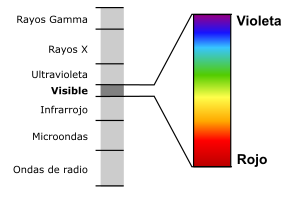
\includegraphics[scale = 0.85]{Imagenes/espectro.png}
\captionof{figure}{\label{fig: Figura1} Gráfico de un espectro electromagnético de la luz visible para el ser humano \cite{IEEEreferencias:Ref48}.} 
	\end{center} 
	 
\end{figure}

Los ojos poseen dos elementos transparentes: la córnea y el cristalino, los cuales dejan pasar la luz hacia la capa interna del ojo llamada retina, que se encuentra en la parte posterior. La retina es una estructura muy compleja, formada por diversos tipos de células interconectadas, donde las únicas que procesan la luz son las células fotorreceptoras, llamadas conos y bastones. Éstas son responsables de detectar la intensidad de la luz y definir el color\cite{IEEEreferencias:Ref12}.

\setlength{\parskip}{2mm}

Entonces, la retina procesa la información recibida por las células fotorreceptoras y la envía en forma de señal eléctrica a través del nervio óptico a la parte trasera del cerebro (lóbulo occipital), donde en conjunto con otro tipo de células cerebrales convierte la información en un impulso nervioso, que percibimos como figuras. Básicamente, la retina procesa una señal luminosa, luego el cerebro decide qué es la imagen \cite{IEEEreferencias:Ref12}.

\setlength{\parskip}{2mm}

La percepción del color inicia al estimular las células en la retina llamadas conos, estos  se concentran principalmente en la mácula de la retina, en donde más al centro se encuentra la fóvea. La visión cromática depende, entre otros factores, de la complejidad del sistema visual que se haya desarrollado durante la evolución. El número de pigmentos visuales y la capacidad de los conos de percibir determinadas longitudes de ondas \cite{IEEEreferencias:Ref12}.

\setlength{\parskip}{2mm}

La visión se clasifica como monocromática (en mapaches y salamandras), dicromática (en la mayoría de los animales), tricromática (en los primates, incluido el humano) y tetracromática (en aves, reptiles y peces). La vista de algunos animales abarca longitudes de onda que sobrepasan ligeramente el espectro visible por los seres humanos, pero se encuentra dentro de los límites generales; por ejemplo, las abejas son sensibles a la luz ultravioleta, que no es percibida por el ojo humano. La visión en los humanos es tricromática debido a que poseemos tres tipos de conos, sensibles al espectro de luz visible correspondiente a los colores azul, verde y rojo. La incidencia en la retina de un haz luminoso de una cierta longitud de onda determina qué tipo de cono ha de estimularse \cite{IEEEreferencias:Ref12}.

\setlength{\parskip}{2mm}

Los conos se denominan según la longitud de onda que los activa: L, M y S (del inglés: long, medium y short) para la percepción de los colores azul, verde y rojo, respectivamente [12]. Cada tipo es sensible a diferentes longitudes de onda o colores. El cono corto tiene el pico de sensibilidad en unos 430 nm. en la zona entre el color violeta y el azul, el cono medio en unos 540 nm. en el color verde y el cono largo tiene el pico en unos 570 nm. casi en el color amarillo. La diferencia entre las señales recibidas de cada uno de los conos permite al cerebro percibir un rango continuo de colores, que es lo que hemos llamado el espectro visible \cite{IEEEreferencias:Ref13}.

\newpage
Después, el cerebro combina la información de cada fotorreceptor y genera los colores intermedios al estimular diferentes conos de manera simultánea \cite{IEEEreferencias:Ref12}.

\setlength{\parskip}{2mm}

Por otra parte, las células fotorreceptoras llamadas bastones pueden funcionar en condiciones de poca luz. Por lo general se localizan en la parte exterior de la retina y se utilizan para la visión periférica\cite{IEEEreferencias:Ref13}.

\setlength{\parskip}{2mm}

Hay un solo tipo de bastones, los cuales son más sensibles a la luz que los conos y son casi enteramente responsables de la visión nocturna. Los bastones no discriminan entre las diferentes longitudes de onda de la luz percibida [12]; tienen el pico de sensibilidad aproximadamete a 498 nm., en la zona entre el verde y el azul. Por lo tanto la visión con los bastones es monocromática \cite{IEEEreferencias:Ref13}.

\setlength{\parskip}{2mm}

Existen dos teorías que explican de mejor manera la percepción del color:

\textbf{a)	Teoría Tricromática (Thomas Young, 1802):}
 Esta teoría hace referencia a que la  percepción visual está dada por la capacidad de los tres tipos de conos existentes (tres mecanismos receptores) a ser estimulados por distintas longitudes de onda\cite{IEEEreferencias:Ref14}.
 
\setlength{\parskip}{2mm} 
 
<<Los tres tipos de pigmentos de los conos (Yodopsina, Cianopsina y Porfiropsina) se corresponderían con los tres mecanismos receptores>>\cite{IEEEreferencias:Ref14}.

\setlength{\parskip}{2mm}

\textbf{b) Teoría de los Procesos Oponentes (Ewald Hering, 1878):}
 
<<Propuso que la naturaleza de la visión del color se debía al emparejamiento de sensaciones de color, que operarían mediante procesos oponentes. Es decir, cada receptor produciría dos tipos de respuestas antagónicas entre sí. Cuando un miembro del par resulta estimulado más que su oponente, entonces se verá el matiz correspondiente al superior, pero si son estimulados por igual, se anulan por ser complementarios y aparece la sensación de gris, como ocurre en la mezcla sustractiva de colores>>\cite{IEEEreferencias:Ref14}.

\subsection{La fototransducción}

El proceso de capturar una señal luminosa y convertirla en una respuesta fisiológica se conoce como fototransducción. La luz es detectada en el ojo por una proteína llamada rodopsina, que se encuentra en la membrana de las células llamadas bastones. La rodopsina está formada por dos partes: una proteína llamada opsina y un pigmento derivado de la vitamina A, conocido como 11-cis-retinal. Este pigmento permite la absorción de la luz al inducir un cambio en su estructura, que a su vez afecta la forma de la proteína rodopsina (cambiando a todo-trans-retinal) \cite{IEEEreferencias:Ref12}.

\setlength{\parskip}{2mm}

El cambio conformacional inducido es el primer paso para que se genere una amplia cascada de señales fisiológicas en las que intervienen diversas proteínas. De esta manera, la rodopsina modificada después interactúa con la proteína transducina, la cual pertenece a un grupo de proteínas llamadas proteínas G, que se activan al unirse con una molécula llamada guanosín trifosfato (GTP). En general, las proteínas G están formadas por tres partes, denominadas subunidades alfa ($\alpha$), beta ($\beta$) y gamma ($\gamma$) \cite{IEEEreferencias:Ref12}. 

\setlength{\parskip}{2mm}

Cuando la transducina se une a GTP, se disocia en dos complejos, la subunidad $\alpha$ unida a GTP
($\alpha$GTP) y el complejo formado por las subunidades $\beta$ y $\gamma$. Luego, la subunidad $\alpha$GTP de la transducina interactúa con la fosfodiesterasa, una proteína que modifica a la molécula derivada del GTP, conocida como guanosín monofosfato cíclico (GMPc). Lo anterior induce la producción de la forma no cíclica de esta molécula (guanosín monofosfato, GMP), que estimula de manera indirecta la producción de GTP para favorecer la amplificación de las cascadas de señales fisiológicas \cite{IEEEreferencias:Ref12}.

\setlength{\parskip}{2mm}

De manera particular, en condiciones de oscuridad o poca luz, la proteína denominada guanilato ciclasa se activa y convierte el GMP en GMPc. Cuando el GMPc se une a ciertas proteínas localizadas en la membrana de las células fotorreceptoras, llamadas canales iónicos dependientes de nucleótidos cíclicos (canales CNG, por sus siglas en inglés), estos canales permiten el paso de iones con cargas positivas (como el calcio o el sodio) hacia el interior de las células, de manera que el flujo de iones también favorece la amplificación de señales al activar o estimular otras proteínas \cite{IEEEreferencias:Ref12} [Figura \ref{fig: Figura2}].

\setlength{\parskip}{2mm}

En los fotorreceptores encontrados en la retina se transforma la luz en un impulso nervioso que luego pasa a las células ganglionares.  Mismo que se irradia al Nervio Óptico el cual se decusa a nivel del Quiasma Óptico \cite{IEEEreferencias:Ref14}, posterior el Nervio Óptico hace sinapsis con las neuronas presentes en el núcleo geniculado lateral (NGL) estructurado histológicamente en capas, comunicadas entre sí. Las dos primeras, constituidas por células magnocelulares, reciben aferencias procedentes de la retina: mientras la capa número uno recibe las de la retina contralateral, la capa número dos lo hace de la retina homolateral al hemicuerpo en que se ubica cada uno de los dos núcleos geniculados laterales encefálicos. Ambas capas son consideradas ventrales con respecto a las siguientes cuatro que les preceden\cite{IEEEreferencias:Ref15}.

\setlength{\parskip}{2mm}

Además de las capas uno y dos que reciben aferencias, cada núcleo geniculado lateral posee otras cuatro capas dorsales compuestas por células parvocelulares. Todas ellas están orientadas a la formación de eferencias destinadas al área cortical 17 de Brodmann, concretamente a la cisura calcarina, para el procesado de la información visual. Las capas pares (capas cuatro y seis) conectan con la capa uno antes mencionada, procesando información de carácter contralateral; por otro lado, las capas impares (tres y cinco) conectan con la dos, trabajando con información ipsilateral. Las eferencias de estos núcleos conforman lo que conocemos con el nombre de radiaciones ópticas o de Gratiolet\cite{IEEEreferencias:Ref15} del cual emergen Radiaciones Ópticas que hacen sinapsis finalmente con las neuronas de la corteza visual, específicamente en el núcleo de Edinger-Westphal \cite{IEEEreferencias:Ref14}.

\setlength{\parskip}{2mm}

\begin{figure}[H]
	\begin{center}
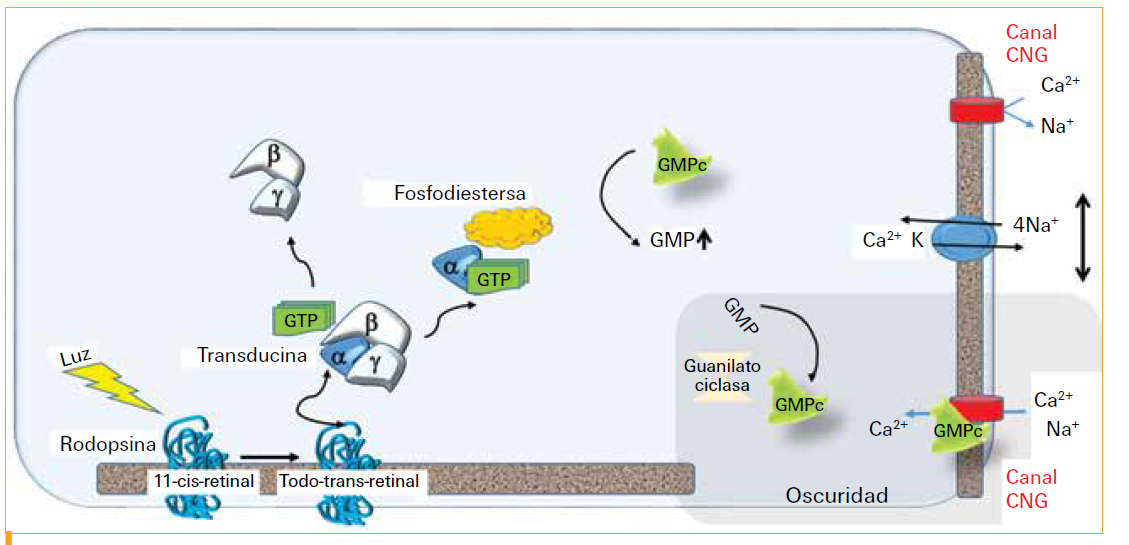
\includegraphics[scale = 0.52]{Imagenes/cascada.png}
\captionof{figure}{\label{fig: Figura2} Cascada de la fototransducción\cite{IEEEreferencias:Ref12}.} 
	\end{center} 
\end{figure}

\subsection{Daltonismo}

La experiencia de cruzar el semáforo, mirar el arcoíris o comprar una camisa, puede ser completamente distinta si eres daltónico
Pero es difícil para quienes no tenemos daltonismo hacernos a la idea de como se ve el mundo sin ciertos colores
El 8\% - 10\% de los hombres y 0.5\% - 1\% de las mujeres tienen daltonismo, normalmente de nacimiento \cite{IEEEreferencias:Ref25}\cite{IEEEreferencias:Ref26}.
Esto significa que prácticamente 1 niño de cada 10 sufrirá una alteración en la visón de los colores", precisa el también director médico de la clínica Área Oftalmológica Avanzada de la ciudad condal, quien sostiene que también se puede heredar de padres a hijos, en la proporción antes descrita\cite{IEEEreferencias:Ref26}.


La prevalencia de alteraciones adquiridas es similar en ambos géneros, pero en alteraciones congénitas el porcentaje es mayor en el género masculino, por la dominancia genética que está ligada al cromosoma X. La prevalencia varía en hombres de 2.5 a 8.7\% y en mujeres de 0.2 a 0.4\% (García y Camacho, 2012; Jiménez et al., 2013; Munaiz, 2012; Cruz-Pérez, 2015; García et al., 2010)\cite{IEEEreferencias:Ref27}.
Las discromatopsias congénitas parecen ser más frecuentes en América del Norte y en Europa occidental, predominando las discromatopsias en varones caucásicos con 5.6\%, siguiendo los asiáticos con 3.1\%, 2.6\% en va- rones hispanos y el grupo de menor prevalencia con 1.4\% pertenece a los afroamericanos (García et al., 2010; Montenegro y Barón, 2011); en cuanto a las mujeres, se obtuvo una prevalencia de 0.5\%\cite{IEEEreferencias:Ref27}.
Otros autores refieren que la prevalencia más alta corresponde a los checos con 10.5\%, estando el resto de Europa alrededor de 8\% y España con 9\% de la población masculina\cite{IEEEreferencias:Ref27}.
Los chinos, japoneses y filipinos presentan una prevalencia de entre 4 y 5\%, los esquimales tienen la cifra más baja con tan sólo 1\% de su población (Lobera, Romero y Carmona, 1992; Valenzuela, 2008. Algunos estudios realizados en México refieren que la prevalencia es entre 2.7 y 6.01\% en varones y 0.5\% en mujeres, predominando en las congénitas el tipo deután y en las adquiridas las tritanomalías (Lagunas, 1984; OMS, 2017; Goldstein, 2011. Difiriendo de estudios que indican también que la prevalencia en México es de 1.9\% en varones y 0.1\% en mujeres (Jiménez et al., 2013). Estas grandes diferencias pueden ser a causa del tamaño de la muestra utilizada. Las frecuencias normalmente altas de 5.43 y 7\% observadas se deben a un alto factor de mestizaje, por eso es necesario tener una muestra significativa, para reducir el margen de error. Es por eso que investigaciones realizadas en México refieren que mientras el grupo sea menos mestizado, más baja es la incidencia de este defecto (Aréchiga, 1976; Jiménez et al., 2013).
Otro estudio sobre incidencia de discromatopsias congénitas en varones en poblaciones indígenas mexicanas muestra un recopilado de estudios de diversas poblaciones, el más antiguo es de 1933 y el último es de 1984. Los datos indican que el porcentaje de incidencia va de 0 a 7.0\%, sin embargo, no se especifican las pruebas utilizadas, el tipo de discromatopsia ni el control que se llevó a cabo para cada estudio (Lagunas, 1984)\cite{IEEEreferencias:Ref27}.
El estudio epidemiológico de discromatopsias congénitas más reciente en México fue realizado por el personal de enfermería en el noreste de México, encontrando una prevalencia de 1.9\%, clasificando los protanes y deutanes en débiles y fuertes (Jiménez et al., 2013)etiquetados. \cite{IEEEreferencias:Ref27}.


El daltonismo es un defecto genético que ocasiona dificultad para distinguir los colores. El grado de afectación es muy variado ya que va desde la dificultad para distinguir cualquier color hasta la dificultad para diferenciar algunos matices del rojo y del verde. En cambio, un daltónico puede apreciar más matices del violeta que un sujeto con visión normal\cite{IEEEreferencias:Ref28}.

Se trata de un proceso con base hereditaria, genética, y que va desde una discreta alteración en la capacidad de distinguir los colores, hasta una dificultad total en discriminar el rojo y el verde [17] siendo la incapacidad de distinguir entre azul y amarillo mucho menos común. Ser completamente daltónico (ver cosas en negro, blanco o tonos grises) es una forma grave del trastorno, llamada acromatopsia. Es extremadamente inusual y va acompañada de una visión generalmente mala\cite{IEEEreferencias:Ref29}.
Eso sí, el doctor Carlos Vergés, director médico del Instituto Oftalmológico Quirónsalud Dexeus, explica a Infosalus que no hay que confundir el daltonismo de origen genético con todas las alteraciones en la visión de los colores.    <<Hay ciertas enfermedades oculares, generalmente las que afectan a la retina y al nervio óptico, que pueden alterar la percepción de los colores. Es lo que se conoce como 'Discromatopsia adquirida' y lo vemos en la retinopatía diabética, las maculopatía,  los casos de glaucoma, además de en ciertas enfermedades neurodegenerativas como el Alzheimer o la esclerosis múltiple>>\cite{IEEEreferencias:Ref26}.

Nathans et al. determinaron que los genes humanos para las opsinas de los conos sensibles a la longitud de onda larga (L) y media (M) están localizados en el cromosoma X (Xq28) y que los genes para la opsina sensible a la longitud de onda corta (S) está ubicado en el cromosoma 7 (7q32). La denominación oficial para designar a los genes de las opsinas de los conos que absorben la longitud de onda L, M y S son OPN1LW, OPN1MW y OPN1SW, respectivamente (Neitz, 2000)\cite{IEEEreferencias:Ref30}.

Así, se reconoce que se trata de un fenómeno más frecuente en hombres que en mujeres porque esta alteración se presenta en el cromosoma 'X', concretamente en un alelo recesivo de este cromosoma, de forma que si lo hereda un hombre ('XY') padecerá daltonismo, mientras que en las mujeres, al ser 'XX', sólo padecerán esta alteración cuando el alelo alterado esté presente en los dos cromosomas\cite{IEEEreferencias:Ref26}.

\subsection{Tipos de Daltonismo}

Aunque existen muchos tipos de daltonismo, el 99\% de los casos corresponden a protanopia y deuteranopia o sus equivalentes (protanomalia y deuteranomalia).

\begin{itemize}
    \item \textbf{Acromático}: El daltonismo acromático es aquel en el que el individuo ve en blanco y negro (escala de gris). El individuo no percibe ningún color ya sea porque no tiene ninguno de los tres tipos de conos o por razones neurológicas. Se presenta únicamente un caso por cada 100.000 personas\cite{IEEEreferencias:Ref31}.
    \item \textbf{Monocromático:} Se presenta cuando \textbf{únicamente existe uno de los tres pigmentos} de los conos y la visión de la luz y el color queda reducida a una dimensión\cite{IEEEreferencias:Ref31}.
    \item \textbf{Dicromático:} El dicromatismo es un defecto moderadamente grave en el cual falta o padece una \textbf{disfunción de uno de los tres mecanismos básicos del color.} Es hereditaria y puede ser de tres tipos diferentes: Protanopia, deuteranopia y tritanopia\cite{IEEEreferencias:Ref31}.

    \begin{itemize}
        \item \textbf{Protanopia.} La protanopia consiste en la ausencia total de los fotorreceptores retinianos del rojo.
        \item \textbf{Deuteranopia.} La ceguera al color verde o deuteranopia se debe a la ausencia de los fotorreceptores retinianos del color verde\cite{IEEEreferencias:Ref31}.
        \item \textbf{Tritanopia.} La tritanopia es una condición muy poco frecuente en la que están ausentes los fotorreceptores de la retina para el color azul \cite{IEEEreferencias:Ref31}[Figura \ref{fig: Figura3}].
    \end{itemize}
    \item \textbf{Tricromático anómalo: } El afectado posee los tres tipos de conos, pero con defectos funcionales, por lo que confunde un color con otro. Es el grupo más abundante y común de daltónicos, tienen tres tipos de conos, pero perciben los tonos de los colores alterados. Suelen tener defectos similares a los daltónicos dicromáticos, pero menos notables. Las afecciones que se incluyen dentro de este grupo son la protanomalia (1\% de los varones, 0.01\% de las mujeres), deuteranomalia, la más usual (6 \% de los varones, 0.4 \% de las mujeres) y tritanomalía muy poco frecuente (0.01 \% de los varones y 0.01 \% de las mujeres)\cite{IEEEreferencias:Ref31}.
\end{itemize}

\begin{figure}[H]
	\begin{center}
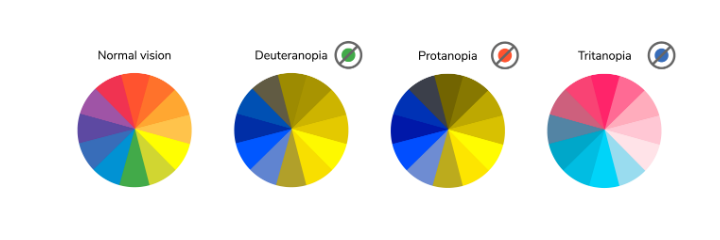
\includegraphics[scale = 0.85]{Imagenes/daltonismo.png}
\captionof{figure}{\label{fig: Figura3} Diferencias entre tipos de daltonismo\cite{IEEEreferencias:Ref25}.} 
	\end{center} 
\end{figure}

\begin{figure}[H]
	\begin{center}
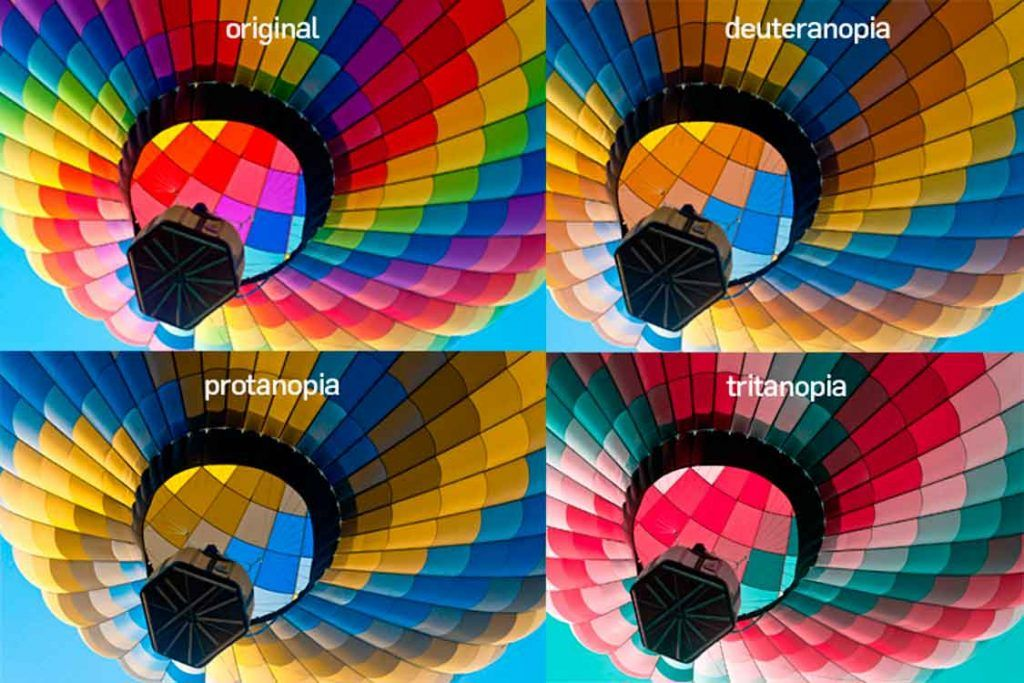
\includegraphics[scale = 0.25]{Imagenes/daltonismo2.jpg}
\captionof{figure}{\label{fig:1} Diferencias en las visiones entre tipos de daltonismo\cite{IEEEreferencias:Ref49}.} 
	\end{center} 
\end{figure}

\newpage

\subsection{Diagnóstico}

El diagnóstico precoz es especialmente importante ahora que hay mecanismos de mejora, como ejercicios de terapia visual, junto a la adaptación de gafas o de lentillas con filtros que nos ayudan a mejorar la visión a estos niños, e incluso adultos\cite{IEEEreferencias:Ref26}.

El daltonismo puede detectarse mediante diferentes test visuales específicos como por ejemplo las Cartas de Ishihara o la test Test de Farnsworth-Munsell\cite{IEEEreferencias:Ref31}.

\textbf{Cartas de Ishihara:} Es el procedimiento más empleado para el diagnóstico del daltonismo y consiste en una serie de 38 láminas en las que es preciso identificar un número que se encuentra insertado en la misma\cite{IEEEreferencias:Ref31}.

Las cartas de Ishihara reciben el nombre en honor a su diseñador, el doctor Shinobu Ishihara, profesor de la Universidad de Tokio, que publicó los primeros ensayos en 1917 y que sirvió como una forma para descifrar si se es daltónico y qué tipo de daltonismo se tiene\cite{IEEEreferencias:Ref30}.
El test se basa en una serie de discos que contienen círculos de puntos de colores de distintos tamaños. En el patrón de puntos se forma un número que resulta visible tan sólo para aquellos con visión normal, mientras que son invisibles o difíciles de descifrar para las personas con defectos de visión. Se trata de una prueba muy simple que hoy día se sigue utilizando\cite{IEEEreferencias:Ref30}.


\begin{figure}[H]
	\begin{center}
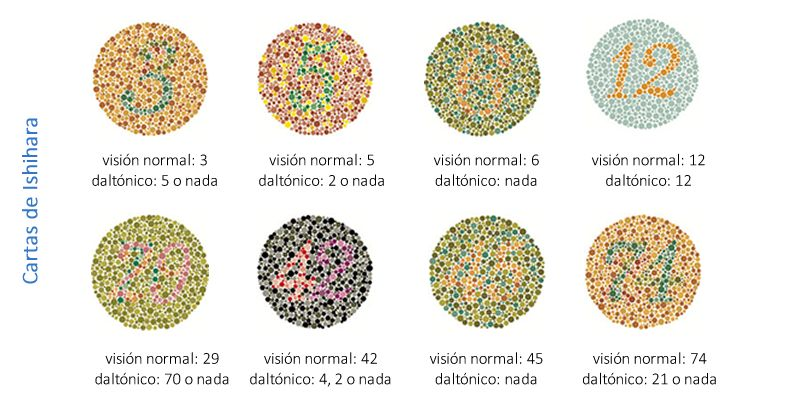
\includegraphics[scale = 0.55]{Imagenes/ishihara.jpg}
\captionof{figure}{\label{fig:1} Ejemplos de cartas de ishihara\cite{IEEEreferencias:Ref50}.} 
	\end{center} 
\end{figure}

\subsubsection{Protanopia y Deuteranopia}

Normalmente, los tonos incluidos en el círculo de las cartas son en tonos azules y verdes, mientras que el número se diferencia en tonos marrones. Esta tipología es utilizada para detectar Protanopia (falta de sensibilidad al color rojo), mientras que la Deuteranopia (ceguera al color verde) se detecta a partir de los círculos en tonos amarillo, naranja y rojo con las figuras de color verde\cite{IEEEreferencias:Ref30}.

\textbf{Test de Farnsworth D15 y D100:} Esta constituido por un conjunto de fichas coloreadas que se diferencian por su tonalidad y están numeradas en el reverso. El paciente debe ordenarlas según la graduación del color.Dentro de las pruebas para el estudio de la visión cromática, el Farnsworth pertenece al grupo de los “Test de colores pigmentarios” (frente a los test de colores espectrales), ya que están constituidos por fichas coloreadas con pigmentos especiales a fin de que presenten una saturación y luminosidad constantes y que difieran solamente por su tonalidad. Recordemos que
saturación, luminosidad y tonalidad son las tres características que definen un color\cite{IEEEreferencias:Ref31}.

\begin{figure}[H]
	\begin{center}
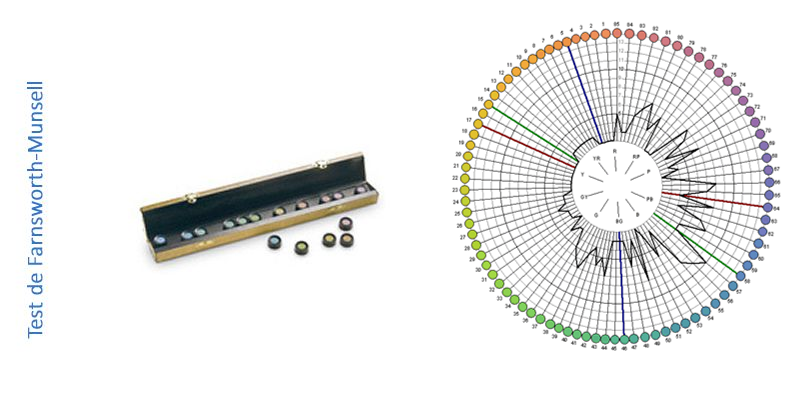
\includegraphics[scale = 0.55]{Imagenes/fm.png}
\captionof{figure}{\label{fig:1}est de Farnsworth } 
	\end{center} 
\end{figure}

\subsection{Tratamiento}
El daltonismo, ¿es sólo cuestión de hombres?

El daltonismo no tiene una curación. Se mantendrá toda la vida pero, generalmente, las personas que lo sufren se acostumbran a este defecto y desarrollan mecanismos de compensación para reconocer los colores. Actualmente, hay gafas y lentillas con filtros adaptados que permiten mejorar la identificación de los colores y ayudan a estas personas en su vida diaria", apostilla el especialista en Oftalmología\cite{IEEEreferencias:Ref26}.

Aun y que no haya una <<cura>> o tratamiento al daltonismo en humanos, existe un avance importante realizado por Mancuso et al. donde lograron corregir este trastorno visual, en un inicio con dos individuos de una especie de mono \textit{<<Saimiri sciureus>>}, por medio de la terapia génica mediada por virus insertando el gen de L-opsina humana (Bennet, 2009). Unos años después, Neitz (2014) señaló que es posible por medio de la misma técnica pasar la visión dicromática a tricromática de algunos primates, adquiriendo la visión del color rojo-verde; de la misma forma, en ratones transgénicos, se logró la visión tricromática añadiendo un tercer tipo de cono \cite{IEEEreferencias:Ref26}.

\subsection{Impacto Social}
Es de vital importancia mencionar este fundamento, ya que de no hacerlo así, estaríamos dejando algo de vitalidad para la herramienta anteriormente mencionada. El impacto social ya se a mencionado implícitamente en los casos de gente reconocida en diferentes ámbitos, ellos comparten diferentes problemas debido a esta alteración.

A continuación desglosaremos de manera más extensa cada uno de las situaciones y los problemas que esta alteración provoca, enunciando de manera precisa estos.

\subsubsection{Comunicación visual}
Asinsten (2010) dice que en todo tipo de comunicación siempre hay tres elementos principales: emisor que es quien produce el mensaje, el receptor quien recibe y comprende o no el mensaje, y el mensaje que contiene la información que se intercambia. De acuerdo a De la Torre y Rizo (2000), el ser humano, como receptor de mensajes, obtiene información a través de sus cinco sentidos, pero cada uno de ellos realiza una función de distinto tipo \cite{IEEEreferencias:Ref32}.

Cada sentido actuando por separado, tiene un solo porcentaje de efectividad, el gusto, el olfato, el tacto y el oído consiguen en conjunto un 20\% de información, mientras que por medio de la vista se capta el 80\% restante. Es por esto que cualquier sistema de comunicación visual tiene tanta importancia. En el caso de la comunicación visual, el emisor será el gráfico o la imagen utilizada, el mensaje el significado portado por la imagen, y el receptor será el que obtenga indirectamente un mensaje por medio de la imagen \cite{IEEEreferencias:Ref32}.

Según De la Torre y Rizo, la información visual es todo lo que puede captar nuestra vista. Todo lo que nuestros ojos ven son emisiones potenciales de mensajes. Munari (1996) acierta que la comunicación visual es todo lo que nuestros ojos ven. Son imágenes que tienen un valor distinto según el contexto en el que se presenten, brindando información diferente. En algunos casos, la comunicación visual es un medio necesario para pasar informaciones de un emisor a un receptor, pero se necesita de muy buena condición para que su funcionamiento y que así no haya falsas interpretaciones. Para lograr esto, es esencial que las dos partes que participen en la comunicación tengan un conocimiento similar del fenómeno \cite{IEEEreferencias:Ref32}.

De acuerdo a ColorAdd (2010), los primeros síntomas del daltonismo se comienzan a detectar en el colegio, cuando surgen dificultades o confusión reconociendo los colores, y es aquí donde se empieza a sentir incompetencia, debido a la exclusión de los demás compañeros\cite{IEEEreferencias:Ref32}.

La deficiencia en la percepción visual y la importancia del color como forma de comunicación puede dificultar el desarrollo del aprendizaje; en México, los estudios sobre discromatopsias son escasos, y es un padecimiento que se cree poco común entre la población, lo que genera des- orientación tanto en las personas con alguna discromatopsia, como en los familiares y profesores sobre el qué hacer (Lobera, Romero y Carmona, 1992; García y Camacho, 2012; Orellana y Sánchez, 2015; Chaves y Carvalho, 2008; Bailey, 2010; Kaleydoscopio, 2014; El Universal, 2008; Aréchiga, 1976; Lagunas, 1984) \cite{IEEEreferencias:Ref27}.

Durante su adultez las personas se enfrentan a un reto mayor, se les prohíbe cursar varias profesiones, como por ejemplo la aviación, la industria gráfica, la industria química, la geología, arqueología, policías, ingenieros, mecánicos ni pilotos de aviación, ya que es necesario tener una buena percepción del color al encargarse del transporte terrestre, aéreo y marítimo. Tampoco pueden acceder a puestos determinados de la industria textil, la fotografía y la pintura, entre otras \cite{IEEEreferencias:Ref32}\cite{IEEEreferencias:Ref1}.

Así con el tiempo, van aumentando las limitaciones mientras la vida se vuelve más completa, se disminuye el ámbito profesional, la realización personal y se pierde el sentido en la integración en la sociedad \cite{IEEEreferencias:Ref32}.

Si bien los expertos reducen el daltonismo a un mal menor, quienes lo padecen difieren: Los problemas derivados del daltonismo son bastantes, aunque puedan parecer superficiales. Hablamos de no poder optar a puestos de trabajo y de tener dificultad para ver a diario \cite{IEEEreferencias:Ref1}
De acuerdo a Matlin y Foley (1996), el color tiene un impacto considerable en la vida diaria. Se considera cómo afecta el color en diferentes productos, como por ejemplo las cajas de detergente deben mostrar colores primarios cálidos, para lograr inspirar imágenes de limpieza y fuera. Con esto, se probó la reacción de consumidores a los detergentes, quienes detectaron que las cajas de color amarillo o naranja eran demasiado fuertes y las de caja azul eran muy débiles, por lo que el producto ideal era utilizar colores claros, blancos y celestes \cite{IEEEreferencias:Ref32}.

\newpage 

\subsection{Discriminación: Una sociedad inadaptada}

Actualmente los daltónicos sufren gran cantidad de limitaciones. Pero, tal como insiste el Dr. Scott Anderson de Oftalmedic, Clínica Salvà, no se derivan de condiciones físicas, sino que están establecidas por la sociedad: \textit{<<Las sociedades se crean a la medida de las mayorías, por eso tenemos códigos de colores para señales de tráfico, semáforos, químicos… Sin embargo una característica de las sociedades modernas es la inclusión creciente de quienes tienen capacidades y necesidades especiales>>}. Es una discriminación indirecta, explica. De hecho, la Asociación de Daltónicos no Anónimos (ASDNA) configura una lista de aquellas profesiones a las que los daltónicos no tienen acceso, entre las que se encuentran la de piloto de aviación, controlador aéreo, conductor de transporte público colectivo, ciertos grados de policía, bombero…
Hay otros ámbitos en los cuales los daltónicos pueden verse desfavorecidos, como en la conducción o la educación. Un fracaso escolar temprano puede deberse al desconocimiento del daltonismo de nuestros hijos, que tienen que estudiar con libros que no están adaptados y sin saber si le ponen una pegatina verde o roja en sus deberes \cite{IEEEreferencias:Ref33}.

El diagnóstico precoz es especialmente importante ahora que hay mecanismos de mejora, como ejercicios de terapia visual, junto a la adaptación de gafas o de lentillas con filtros que nos ayudan a mejorar la visión a estos niños, e incluso adultos y con ello lograr una inclusión social \cite{IEEEreferencias:Ref26}.

En definitiva, tal y como asegura el Dr. Scott Anderson, <<las sociedades deberían enfocarse a ofrecer igualdad de posibilidades, pero a cada cual según su capacidad o condición>>. Al fin y al cabo el mundo es el mismo para todos, aunque algunos lo vean de otro color \cite{IEEEreferencias:Ref33}.

Avanzando con el tema, es propio también mencionar la teoría de las tecnologías básicas a emplear en el sistema, ya que ellas serán las que nos ayudarán a que el proyecto logre su cometido.

Las dos que se hará mención son el árbol de decisiones, algoritmo de \textit{machine learning} capaz de lograr hacer el diagnóstico exacto y el modelo RGB, el cual nos ayudará entender en la teoría para aplicarlo en la transformación de colores. 


\subsection{Árbol de decisión}

El enfoque  Classification And Regression Tree (Árbol de regresión y Clasificación) (CART) fue desarrollado por Breiman et al. (1984)\cite{IEEEreferencias:Ref44}.

\begin{itemize}
    \item Son un tipo de algoritmos de \textit{\textbf{machine learning}} de aprendizaje supervisado (i.e., existe una variable objetivo predefinida).
    \item Principalmente usados en problemas de clasificación.
    \item Las variables de entrada y salida pueden ser categóricas o continuas.
    \item Divide el espacio de predictores (variables independientes) en regiones distintas y no sobrepuestas \cite{IEEEreferencias:Ref44}.
\end{itemize}

Veamos a continuación a introducir las ideas fundamentales del denominado algoritmo \textit{Top Down Induction of Decision Trees}(TDIDT ) el cual puede ser contemplado como uniformizador de la mayoría de los algoritmos de inducción de arboles de clasificación a partir de un conjunto de datos conteniendo patrones etiquetados\cite{IEEEreferencias:Ref15}.

\begin{figure}[H]
	\begin{center}
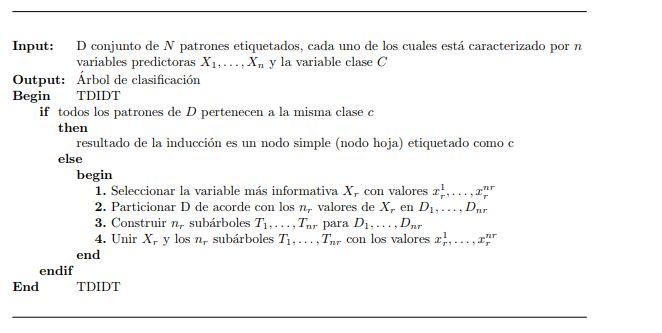
\includegraphics[scale = 0.85]{Imagenes/algoritmo.JPG}
\captionof{figure}{\label{fig:7} pseudocódigo de el algoritmo más básico del árbol de decisión\cite{IEEEreferencias:Ref46}.} 
	\end{center} 
\end{figure}

\setlength{\parskip}{2mm}

\textbf{Explicación:}

Árbol inicial:

Árbol con un único nodo, sin etiquetar, al que asignamos como conjunto de ejemplos todo el conjunto de entrenamiento.

\setlength{\parskip}{2mm}

• Bucle principal:

\setlength{\parskip}{2mm}

– Consideramos el primer nodo, N, sin etiquetar
\setlength{\parskip}{2mm}

$\ast$ Si los ejemplos asignados N tienen todos la misma clasificación,  etiquetamos N con esa clasificación.

\setlength{\parskip}{2mm}

$\ast$ En otro caso ...

\setlength{\parskip}{2mm}

· Etiquetamos N con el mejor atributo A según el conjunto de
ejemplos asignado.
\setlength{\parskip}{2mm}

· Para cada valor de A creamos una nueva arista descendente en el nodo N, y al final de cada una de esas nuevas aristas creamos un nuevo nodo sin etiquetar, N1, . . . , Nk.

\setlength{\parskip}{2mm}

· Separamos los ejemplos asignados al nodo N según el valor que tomen para el atributo A y creamos nuevos conjuntos de ejemplos para N1, . . . , Nk.


\setlength{\parskip}{2mm}

• Hasta que todos los nodos estén etiquetados \cite{IEEEreferencias:Ref15}.

Subyacente al algoritmo TDIDT es que mientras que todos los patrones que se correspondan con una determinada rama del árbol de clasificación no pertenezcan a una misma clase, se seleccione la variable que de entre las no seleccionadas en esa rama sea la más informativa o la más idónea con respecto de un criterio previamente establecido. La elección de esta variable sirve para expandir el árbol en tantas ramas como posibles valores toma dicha variable\cite{IEEEreferencias:Ref15}.

La decisión de hacer divisiones estratégicas afecta altamente la precisión del árbol \cite{IEEEreferencias:Ref44}.

\begin{itemize}
    \item Los criterios de decisión son diferentes para árboles de clasificación y regresión.
    \item Existen varios algoritmos para decidir la ramificación.
    \item La creación de subnodos incrementa la homogeneidad de los subnodos resultantes. Es decir, la pureza del nodo se incrementa respecto a la variable objetivo.
    \item  Se prueba la división con todas las variables y se escoge la que produce subnodos más homogéneos.
    \item Algunos algoritmos más comunes para la selección: Indice Gini, Chi Cuadrado, Ganancia de la información y Reducción en la varianza \cite{IEEEreferencias:Ref44}.

\end{itemize}

\subsubsection{Selección y expansión}

Evidentemente, la construcción del árbol de decisión no es única, y si aplicamos una estrategia u otra a la hora de decidir en qué orden se hacen las preguntas sobre los atributos podemos encontrar árboles muy dispares. De entre todos los posibles árboles, estamos interesados en encontrar aquellos que cumplan las mejores características como máquinas de predicción, e intentaremos dar un mecanismo automático de construcción del árbol a partir de los ejemplos\cite{IEEEreferencias:Ref45}.

En el año 1979, J. Ross Quinlan presenta un método para construir árboles de decisión que presentan muy buenas características, como son un buen balanceado y un tamaño pequeño (el menor número de preguntas posibles para poder encontrar la respuesta en todos los casos, si es posible). Para ello, hace uso de la Teoría de la Información desarrollada por C. Shannon en 1948. Aunque el mérito se le asocia a Quinlan, la verdad es que de forma paralela aparecieron varios métodos de construcción que eran prácticamente equivalentes. El algoritmo de construcción que presenta se llama ID3, y hasta el momento ha sido el más utilizado y en el que se han basado la mayoría de las mejoras posteriores introducidas por el mismo Quinlan y por otros autores\cite{IEEEreferencias:Ref45}.

El ID3 construye un árbol de decisión de arriba a abajo, de forma directa, sin hacer uso de backtracking, y basándose únicamente en los ejemplos iniciales proporcionados. Para ello, usa el concepto de Ganancia de Información para seleccionar el atributo más útil en cada paso. En cierta forma, sigue un método voraz para decidir la pregunta que mayor ganancia da en cada paso, es decir, aquella que permite separar mejor los ejemplos respecto a la clasificación final\cite{IEEEreferencias:Ref45}..

Para poder aplicar el algoritmo hemos de comenzar sabiendo cómo se mide la ganancia de información, y para ello hay que introducir el concepto de Entropía de Shannon, que de alguna forma mide el grado de incertidumbre de una muestra\cite{IEEEreferencias:Ref45}.

\textbf{Entropía de Shannon}

Supongamos que miramos cómo de homogéneos son los ejemplos de los que queremos aprender respecto a la clasificación:
\begin{itemize}
    \item Una muestra \textbf{completamente homogénea} (es decir, en la que todos se clasifican igual) tiene incertidumbre mínima, es decir, no tenemos dudas de cuál es la clasificación de cualquiera de sus elementos (si elegimos al azar cualquier de ellos, sabremos qué resultado tendremos). En este caso, fijaremos la incertidumbre (entropía) a 0\cite{IEEEreferencias:Ref45}.
    \item Una muestra \textbf{igualmente distribuida}, es decir, que tiene el mismo número de ejemplos de cada posible clasificación, muestra una incertidumbre máxima, en el sentido de que es la peor situación para poder saber a priori cuál sería la clasificación de cualquiera de sus ejemplos elegido al azar. Así pues, en este caso fijaremos la incertidumbre (entropía) a 1\cite{IEEEreferencias:Ref45}.
\end{itemize}
Con estos requisitos, y algunas propiedades más que hemos de añadir para que se comporte bien, buscamos dar una definición matemática de la entropía que sirva para medir la incertidumbre de un sistema. Tras un análisis minucioso de las propiedades que debía cumplir una tal función de entropía, Shannon llegó a la conclusión de que la mejor función matemática que mide este grado de incertidumbre es la siguiente:
 \begin{equation}\label{eq:ej}
E(S) = \sum_{i=1}^{C}-p_{i}log_{2}(p_{i})
\end{equation}

donde \textit{S} es el conjunto de muestras (el sistema analizado), \textit{C} es el número de diferentes clasificaciones que usamos, y cada $p_{i}$ es la proporción de ejemplos que hay de la clasificación i en la muestra.

\subsubsection{Poda}

\begin{itemize}
    \item \textbf{Pre-poda.} Estimar si es probable que se produzca una mejora si se expande el nodo actual. Si no es probable, el nodo no se expande\cite{IEEEreferencias:Ref46}.
   \item \textbf{Post-poda.} Dado un árbol de decisión, se poda un subárbol (convirtiéndolo en un nodo hoja con valor de clase igual a la clase más
    frecuente en el correspondiente nodo) si su poda produce un árbol
con mejor rendimiento que el inicial. El proceso de poda comienza
desde los nodos más profundos del árbol escogiendo, a igual nivel, el
que produzca un mayor rendimiento\cite{IEEEreferencias:Ref46}.

\end{itemize}

Para el aspecto de los filtros, realizaremos una transformación de colores, este nos permitirá colocar filtros sobre una imagen, emulando de manera cercana la visión real del color. 

Por lo que es importante hablar del modelo y como este debe ser transformado para llegar a lograr esto.

\subsection{Modelo RGB}

Módelo euclideano creado originalmente para los televisores NTSC (National Television System(s) Committee), el cual buscaba ser compatible con las televisiones de Blanco y Negro de la época \cite{IEEEreferencias:Ref16}.

Los colores aparecen con sus componentes primarias de rojo, verde y azul. Los valores de R, G, y B se encuentran a lo largo de tres ejes. En otras palabras, en el eje del rojo, en el eje del verde y en el eje del azul se encuentran las intensidades de cada color. El cián está situado en el vértice del cubo en donde el color verde y el azul tienen su máximo valor, y el valor del rojo es cero \cite{IEEEreferencias:Ref16}.
\begin{figure}[H]
	\begin{center}
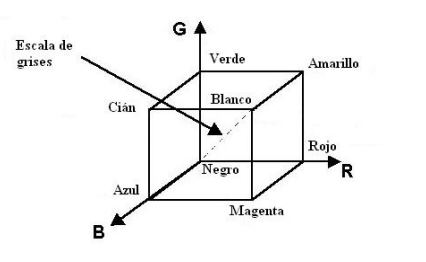
\includegraphics[scale = 0.85]{Imagenes/cubo.JPG}
\captionof{figure}{\label{fig:8} Cubo unitario de colores en RGB \cite{IEEEreferencias:Ref47}.} 
	\end{center} 
\end{figure}

\subsection{Segmentación del color}

La adquisición de la información se realiza a través imagen
en color obtenida, a continuación, se obtiene la
imagen de luminancia de la imagen original y la imagen en
escala de grises de la componente de color que queramos captar.
Posteriormente realizamos una substracción de la información
que contiene la imagen de luminancia de la imagen original
sobre la imagen de escala de grises de la componente a captar.
Lo que se obtiene con esto, es una imagen en escala de grises en
la cual quedan resaltados los objetos del color de la componente
deseada \cite{IEEEreferencias:Ref47}.

\begin{figure}[H]
	\begin{center}
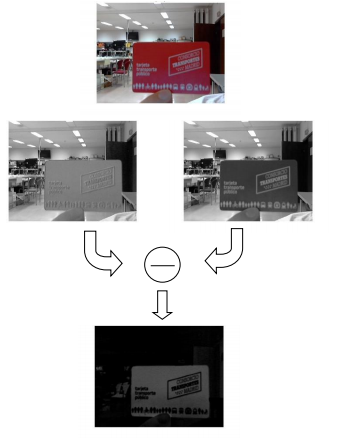
\includegraphics[scale = 0.85]{Imagenes/segmentacion.png}
\captionof{figure}{\label{fig:1}  Ejemplo reconocimiento color rojo. Imagen original (arriba), imagen luminancia banda de color (centro izquierda, imagen luminancia original (centro derecha) e imagen diferencia (abajo)\cite{IEEEreferencias:Ref47}} 
	\end{center} 
\end{figure}

Hay que tener en cuenta que para calcular la señal de luminancia de la imagen original.

\begin{equation}\label{eq:ej}
Y = 0.299R + 0.587G + 0.114B 
\end{equation}

Donde: \textit{Y} es el valor del color del pixel, y \textit{R,G y B}, solo sirven para muestrar el valor de cada uno de los canales del RGB.

Como vemos la imagen de luminancia va a contener una
mayor influencia por parte de la componente verde en relación-
a las otras. A la hora de hacer la substracción anteriormente
explicada, el objetivo deseado es obtener la máxima diferencia
(mayor brillo en la imagen de diferencia) para la componente a
extraer. Esto nos permitirá una mejor identificación de los
objetivos a seguir en el \textit{tracking}\cite{IEEEreferencias:Ref47}.

A partir de la imagen puede apreciar que no todas las
componentes van a proporcionar la misma imagen diferencia, en
concreto en la componente verde existe una diferencia mucho
más precaria, lo cual se habrá de considerar en la etapa de
procesado\cite{IEEEreferencias:Ref47}. 

\section{Estado del Arte}
Existen aplicaciones desarrolladas por grandes emporios que buscan brindarle a una persona que padece daltonismo, algún tipo de apoyo, por lo que encontrar herramientas que se apoyen de los sistemas computacionales es muy complicado. 

Es considerable apoyarse de las tecnologías para ayudar a brindar una mejor calidad de vida a las personas daltónicas. A continuación mostraremos el estado de arte, describiendo aquellas aplicaciones y/o contribuciones que se hacen fundamentales para el diseño de la herramienta.

\subsection{ColorADD}

El denominado <<código braile para los daltónicos>>, es un código único, inclusivo, universal basado en tres símbolos monocromáticos que representan a los colores primarios, que permite la interpretación del color. A través del conocimiento de la <<Teoría de la Adición del Color>> que se enseña en los años escolares tempranos, los símbolos pueden estar relacionados y toda la paleta de colores se identifica gráficamente\cite{IEEEreferencias:Ref17}.
\newline
\begin{figure}[H]
	\begin{center}
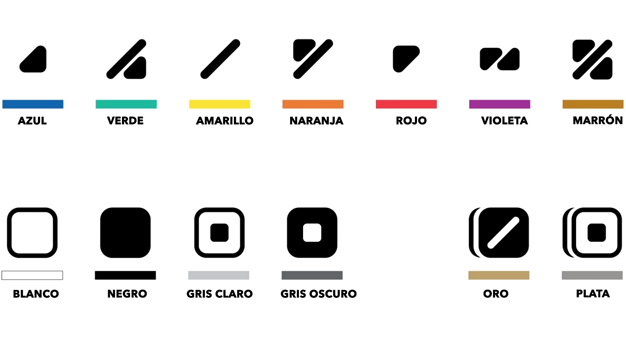
\includegraphics[scale = 0.65]{Imagenes/coloradd.PNG}
\captionof{figure}{\label{fig:10} Código de colores ColorADD\cite{IEEEreferencias:Ref50}} 
	\end{center} 
\end{figure}

Como dice Miguel Neiva creador de ColorADD tras ocho años de investigación, \textit{<<Los símbolos que incluyen los colores, se convierten en un juego mental, fácil de memorizar y aplicar en situaciones cotidianas. ColorADD es un herramienta democrática e inclusiva que acerca el color y el diseño a todos>>}\cite{IEEEreferencias:Ref17}. \newline

Un dato curioso es el país de Portugal, el cual a día de hoy señaliza todas sus lineas de metro de Oporto con este código de colores, además de que siete hospitales portugueses lo usan tanto en la señalización interna, como en las pulseras de los pacientes, o en las etiquetas de las jeringuillas de análisis y contar con mapas turísticos con esta señalización del código \cite{IEEEreferencias:Ref17}.


\begin{figure}[H]
	\begin{center}
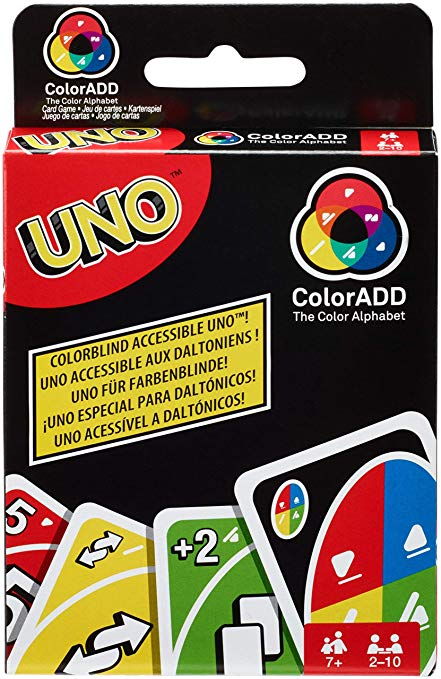
\includegraphics[scale = 0.14]{Imagenes/UNO.jpg}
\captionof{figure}{\label{fig:1} Juego con código colorADD\cite{IEEEreferencias:Ref17}} 
	\end{center} 
\end{figure}

De igual manera las empresas Viarco y Mattel generaron apoyándose del código ColorADD, su primer paquetes de colores aptos para ciegos de color y un juego UNO (juego muy conocido de Mattel en el que a través de números y colores van bajando cartas hasta que a algún jugador sólo le quede una) con este código de colores.   

\begin{figure}[H]
	\begin{center}
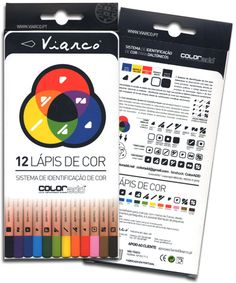
\includegraphics[scale = 0.45]{Imagenes/coloradd.jpg}
\captionof{figure}{\label{fig:1} Colores Viarco con código ColorADD \cite{IEEEreferencias:Ref17}} 
	\end{center} 
\end{figure}

\subsection{Microsoft\textregistered \space Color Binacoulars }
En el año 2016 la marca americana Microsoft\textregistered,\space a través de su programa Microsoft\textregistered \space Garage que alienta a los empleados a trabajar en proyectos que les apasionan, incluso si no tienen ninguna relación con su función principal dentro de la empresa, desarrolló un proyecto llamado Microsoft Color binacoulars, el cual en palabras de sus mismos creadores:

\setlength{\parskip}{2mm}

\textit{<<Color Binoculars ayuda a las personas daltónicas a distinguir entre los colores en su vida cotidiana. Usando su cámara, los binoculares de color reemplazan combinaciones de colores difíciles, como el rojo y el verde, con combinaciones más fáciles de distinguir, como el rosa y el verde>>} \cite{IEEEreferencias:Ref18}.

\setlength{\parskip}{2mm}

\textit{<<La aplicación también es compatible con los tres tipos principales de daltonismo. Ya sea que elija flores para un ser querido, experimente la belleza de la naturaleza o elija ropa a juego para su atuendo, deje que Color Binoculars lo ayude a ver mejor su mundo  >>} \cite{IEEEreferencias:Ref18}.

\setlength{\parskip}{2mm}

El funcionamiento de la aplicación es algo sencillo, se trata de una aplicación móvil, la cual proporciona un cambio de colores a través de un filtrado de la cámara del teléfono inteligente, dándole un acercamiento de entre los tres tipos de ceguera de colores disponibles, Verde/Rojo, Rojo/Verde, Azul/Amarillo \cite{IEEEreferencias:Ref18}.

\begin{figure}[H]
	\begin{center}
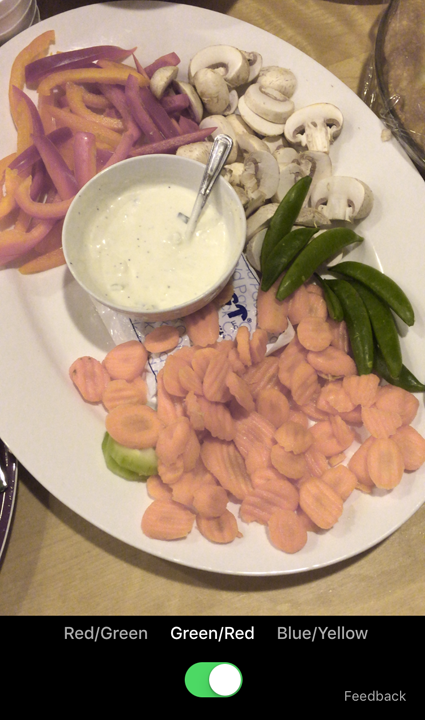
\includegraphics[scale =0.25]{Imagenes/Color_Binoculars_03-1.png}
\captionof{figure}{\label{fig:1} Captura de pantalla de la aplicación en funcionamiento\cite{IEEEreferencias:Ref18}} 
	\end{center} 
\end{figure}

\subsection{Samsung\textregistered \space SeeColors }

A finales del año 2017 la marca de electrónicos coreana Samsung\textregistered,\space dio a conocer una aplicación en su propio portal web de noticias, el cual ellos mismos lo describieron como <<Se trata de una herramienta que ayuda las personas con con deficiencia de visión de color (CVD, por sus siglas en inglés) a identificar sus deficiencias visuales personales. QLED TV, con un volumen de color del 100\%, ajusta la configuración de color en la pantalla, con base en los resultados individuales, y permite que los espectadores con CVD disfruten de una experiencia de visualización con colores optimizados>> \cite{IEEEreferencias:Ref19}. \newline

\setlength{\parskip}{2mm}

Esta herramienta funciona desde una aplicación móvil, la cual detecta de manera personalizada a la deficiencia de colores que la persona padece, para después brindarle una recalibración de los colores en la proyección de las pantallas QLED TV de la marca Samsung\textregistered \cite{IEEEreferencias:Ref19}. \newline

\setlength{\parskip}{2mm}

Para ofrecer un método fácil que determine de qué manera mira cada persona los colores, Samsung Electronics colaboró con la Profesora Klára Wenzel, directora del Departamento de Mecatrónica, Óptica e Ingeniería Mecánica e Informática de la Universidad de Tecnología y Economía de Budapest, para incorporar Colorlite Test (Prueba de Visión Cromática) o C-Test (Prueba C), a los televisores y los dispositivos móviles.
\cite{IEEEreferencias:Ref19}.

\setlength{\parskip}{2mm}

A continuación se mostrará un diagrama que la misma marca proporciona en su portal de noticias. \newline

\begin{figure}[H]
	\begin{center}
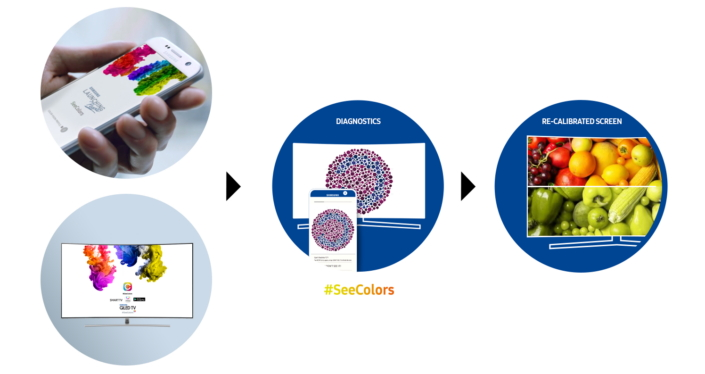
\includegraphics[scale = 1.40]{Imagenes/Samsung-SeeColors-App-for-QLED-TV_main_2.jpg}
\captionof{figure}{\label{fig:13} Diagrama a alto nivel de el proceso de funcionamiento de la aplicación Samsung\textregistered \space SeeColors \cite{IEEEreferencias:Ref19}} 
	\end{center} 
\end{figure}

\subsection{Visolve}

Bajo la misma inforamción encontrada en la página web de la herramienta, ella se define como la herramienta de software que transforma los colores de la pantalla de la computadora en colores discriminables para varias personas, incluidas las personas con deficiencia de la visión del color, comúnmente llamada daltonismo. Además de la conversión de color, también tiene capacidades de filtrado y eclosión de color \cite{IEEEreferencias:Ref20}.

\setlength{\parskip}{2mm}

Visolve es una herramienta instalable en varios dispositivos, tanto moviles, como computadoras, ya que se encuentra un instalador en Windows y Mac, como en Android y IOS \cite{IEEEreferencias:Ref20}.

\setlength{\parskip}{2mm}

Además de distinguir colores y encontrar un color específico, su objetivo es ayudar a las personas con daltonismo: adivinar un color normal, y sentir las gradaciones de color en paisajes naturales, etc. por su información visual.
\cite{IEEEreferencias:Ref20}.

\setlength{\parskip}{2mm}

Visolve puede ejecutar los siguientes tres tipos de transformación de color, filtrado y sombreado:

\begin{itemize}
    \item Transformación rojo-verde: transforma los colores más rojos en más brillantes y los colores más verdes en más oscuros,
    \item Transformación azul-amarilla: transforma los colores más azules en más brillantes y los colores más amarillos en más oscuros,
    \item Aumento de saturación: aumenta la saturación de todos los colores.
    \item Filtrado: oscurece todos los colores que no sean el color especificado, y
    \item Trama: dibuja diferentes patrones de trama según el color
\cite{IEEEreferencias:Ref20}.
\end{itemize}

Cuando las personas con daltonismo aplican, por ejemplo, la transformación Rojo-Verde, si tienen en cuenta la regla de transformación anterior y ven cambios de color, podrían adivinar un color normal. Además, la transformación Rojo-Verde refleja el grado de saturación de color en su brillo regularmente. Entonces podrían saber no solo la diferencia entre rojo y verde, sino también la diferencia entre dos rojos, es decir, los grados de rojo\cite{IEEEreferencias:Ref20}.

\setlength{\parskip}{2mm}

Esperamos que el diseño universal de visión en color se incorpore en cada dispositivo digital con pantalla. Además, podemos ayudar a que su sitio web sea más accesible.
\cite{IEEEreferencias:Ref20}.

\newpage
\section{Propuesta}

\subsection{Planteamiento del problema}

El daltonismo es un problema, social,laboral, personal, familiar y médico poco atendido debido a que se trata de una alteración y no de una enfermedad, el cual como se definió en el marco teórico, se trata de una alteración congénita o adquirida que afecta la visión de colores, provocando problemas a todo aquel que la padece.

Para fines de este proyecto, se planteará como alcance solamente a la personas que padecen daltonismo congénito, ya que representa un mayor esfuerzo en aquellas que son por vía adquirida, debido a que como se estipula en el marco teórico estos no cumplen con las mismas características.

Se tiene que dejar como precedente, que el paciente-médico siempre debe ser visto como un solo ente, por lo que en el proyecto el paciente-oftalmólogo será presentado de esta manera, debido a que todo aquello que represente una mejora para cualquier personal del área médica(para fines del proyecto el oftalmólogo), presentará sustancialmente un impacto positivo para el paciente.

Así que su principal virtud será evitar casi en su totalidad el error humano del oftalmólogo producido por diferentes factores tales como, cansancio debido a largas jornadas de trabajo, distracciones, etc. Evitando así el crearle un falso diagnóstico de daltonismo a un paciente.

Vale la pena recalcar por último, que es primordial, más no necesario, que este sea implementado como primera vía a niños en edad temprana, para sí se tenga un conocimiento certero de que este padece daltonismo, apoyando de diversas maneras a que la persona aminore su problema a una etapa adulta buscando alternativas que lo ayuden en su día a día.

\subsection{Justificación}

Desde que John Dalton lo descubriese en sí mismo el 1792 \cite{IEEEreferencias:Ref2} a la fecha, se han realizado pocos estudios sobre el tema, al igual que lo poco que se ha diseñado en sistemas sobre el mismo. La mayor parte de la gente ignora padecer daltonismo. Si bien no es una enfermedad tiende a ser un problema de carácter médico, social y profesional. Una alternativa viable y poco ocupada es los sistemas, estos no pueden curar la alteración, pero sí pueden auxiliar de manera viable al uso de más herramientas para los oftalmólogos, los cuales pueden diagnosticar a través de del algoritmo de clasificación supervisada, de inteligencia artificial. Así que nuestro enfoque principal será el uso médico. Apoyando a mostrar el espectro real de colores a aquellos que acudan a consulta, logrando aminorar la marginación social provocada por la alteración, la cual ocurre cuando es expuesta la persona por sus grupos cercanos y/o familiares causando burlas, rezago y/o discriminación, acompañada de la limitante para desempeñar ciertos empleos.

\subsection{Metodología}
La metodología elegida bajo el que se creará este diseño es SCRUM, metodología con base en el paradigma ágil, que reduce la complejidad en el desarrollo de productos para satisfacer las necesidades de los clientes. La gerencia y los equipos de Scrum trabajan juntos alrededor de requisitos y tecnologías para entregar productos funcionando de manera incremental usando el empirismo. 

Cabe mencionar algunas definiciones con las que cuenta esta metodología trabaja, las cuales no servirán para el desenvolvimiento del trabajo.

\begin{figure}[H]
	\begin{center}
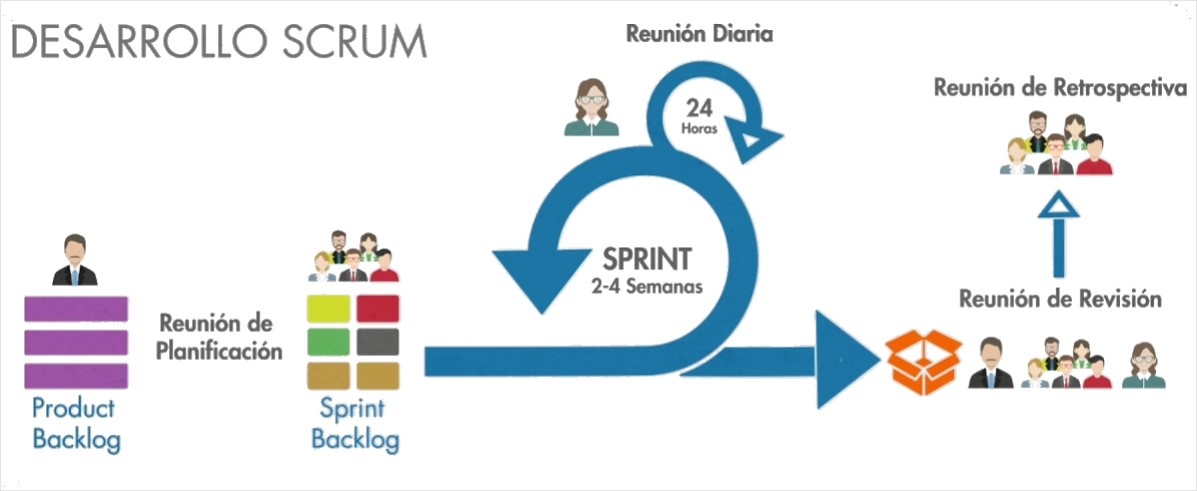
\includegraphics[scale = 0.40]{Imagenes/desarrollo_scrum.jpg}
\captionof{figure}{\label{fig:2} Ciclo de vida de un proyecto en SCRUM \cite{IEEEreferencias:Ref51}} 
	\end{center} 
\end{figure}

\subsubsection{SCRUM}
Scrum es un marco de trabajo simple que promueve la colaboración en los equipos para lograr desarrollar productos complejos. Ken Schwaber y Jeff Sutherland han escrito La Guía Scrum para explicar Scrum de manera clara y simple \cite{IEEEreferencias:Ref21}. \newline

\setlength{\parskip}{2mm}

Scrum no cuenta con requerimientos funcionales y no funcionales, a su vez este cuenta con un mecanismo llamado épicas e historias de usuario, las historias de usuario se crean de redacciones hechas por uno o más integrantes del \textit{scrum core}, mientras que las épicas con los resultados obtenidas de esta \cite{IEEEreferencias:Ref21}.\newline

\setlength{\parskip}{2mm}

Scrum tiene como principal activdad los \textit{Sprints}, a estos se les define un tiempo llamado \textit{<<TimeBox>>} el cual, se puede ir monitoreando a través de dos artefactos, la \textit{burndown chart} y realizando actualizaciones al \textit{backlog}, además de llevar un seguimiento en reuniones llamadas \textit{daily standup}, las cuales son reuniones de una duración menor a 15 minutos, en la que se designan las tareas y se les pregunta del avance de las tareas al \textit{scrum core}, en caso de haber un retraso, el \textit{scrum master}, el cual se designa del ser el más preparado de los integrantes del \textit{scrum core}, con el fin de acabar en el tiempo propuesto al inicio del \textit{sprint} \cite{IEEEreferencias:Ref21}.\newline

\setlength{\parskip}{2mm}

Al finalizar cada uno de los \textit{sprints}, debe de encontrarse un entregable, el cual se conforma del mínimo entregable definido por el alcance del \textit{sprint}, después de realizar el entregable, se realizar un \textit{Sprint Review}, el cual sirve para dar una retrospectiva obtenida por el sprint, analizando cuales fueron errores y aciertos en la planeación del \textit{sprint} \cite{IEEEreferencias:Ref21}.\newline

\subsubsection{BurnDown Chart}
BurnDown Chart, o Gráfo de trabajo pendiente, es una gráfica en la cual se muestra la velocidad en la que se está terminando los objetivos y/o tareas planeadas en el sprint. Sirve como una buena métrica para medir si esta ocurriendo un atraso en el proyecto \cite{IEEEreferencias:Ref22}.

\subsubsection{Backlog}
El cliente es el responsable de crear y gestionar la lista (con la ayuda del Facilitador y del equipo, quien proporciona el coste estimado de completar cada requisito). Dado que reflejar las expectativas del cliente, esta lista permite involucrarle en la dirección de los resultados del producto o proyecto \cite{IEEEreferencias:Ref23}.
\newpage
\begin{itemize}
    \item Contiene los objetivos/requisitos de alto nivel del producto o proyecto, que se suelen expresar en forma de historias de usuario. Para cada objetivo/requisito se indica el valor que aporta al cliente y el coste estimado de completarlo. La lista está priorizada balanceando el valor que cada requisito aporta al negocio frente al coste estimado que tiene su desarrollo, es decir, basándose en el Retorno de la Inversión (ROI).
    
    \item En la lista se indican las posibles iteraciones y las entregas (releases) esperadas por el cliente (los puntos en los cuales desea que se le entreguen los objetivos/requisitos completados hasta ese momento), en función de la velocidad de desarrollo del (los) equipo(s) que trabajará(n) en el proyecto. Es conveniente que el contenido de cada iteración tenga una coherencia, de manera que se reduzca el esfuerzo de completar todos sus objetivos.
    \item La lista también tiene que considerar los riesgos del proyecto e incluir los requisitos o tareas necesarios para mitigarlos\cite{IEEEreferencias:Ref23}.

\end{itemize}

\subsubsection{Sprint}
Son ciclos de ejecución muy cortos, los cuales son creados, gestionados y ejecutados por el mismo scrum core, cada de uno de ellos se compone de varias fases, y al finalizarlos resulta un entregable. \cite{IEEEreferencias:Ref21}.

\subsubsection{Daily StandUp}
Es una reunión por parte del \textit{Scrum Team}, de duración máxima de 15 minutos, en la que se detallan los avances designados a el \textit{scrum team} así como los problemas que podrían estar presentes \cite{IEEEreferencias:Ref21}.

\setlength{\parskip}{2mm}

Es importante que estas reuniones no rebasen los 15 minutos, ya que podrían afectar el seguimiento del \textit{Sprint} \cite{IEEEreferencias:Ref24}.

\setlength{\parskip}{2mm}

Cabe recalcar que dentro de SCRUM existen diferente roles, tales como:
\begin{itemize}
    \item \textbf{Product Owner:} Es el enlace entre el \textit{scrum team} y los \textit{stake holders}.
    \item \textbf{Stake Holder:} Son los interesados en el proyecto, no pertenecientes al \textit{Scrum Team}, ya sean clientes, patrocinadores, directores, etc.
    \item \textbf{Scrum Master:} Es la persona con más experiencia dentro del \textit{SCRUM Team}, por ende es el encargado de resolver los problemas más difíciles que ocurran dentro del \textit{Sprint}, así como apoyar y dar seguimiento al proyecto.
    \item \textbf{Scrum Team:} Son todos los integrantes directamente involucrados con el proyecto \cite{IEEEreferencias:Ref24}.
\end{itemize}

Una manera fácil, viable y sencilla de obtener requerimientos es proporcionada por Scrum, ya que se encuentran disponibles un par de ellas que van de la mano y ayudan al análisis del \textit{Asis}. Este par de recursos son: 

\begin{itemize}
    \item \textbf{Historias de usuario:} Son historias redactadas por el \textit{scrum team}, respondiendo a las preguntas, ¿Quién?, ¿Cómo? y ¿Para qué?
    \item \textbf{Épicas:} Es el concentrado final de las historias de usuario, el cúal solamente pronuncia los objetivos (Requerimientos funcionales y no funcionales) a seguir del proyecto \cite{IEEEreferencias:Ref24}.
\end{itemize}
\newpage
\subsubsection{Justificación del uso de la metodología}

El modelo ágil es uno de los más ocupados hoy en día en las empresas, es un modelo que te permite sacar proyectos auto gestionados de manera muy rápida, debido a que sus sprint son muy prácticos es una metodología muy amplia en lo que hace, ya que te permite retomar tareas de entregables anteriores, si es que uno omitió u olvidó incluirlo en el alcance de ese sprint.

\textit{SCRUM} también cuenta con herramientas como las anteriormente mencionadas que nos ayudan a poder administrar el proyecto de manera correcta y concisa.

\subsubsection{Sprints del proyecto}
Para cerrar el tema, la propuesta de actividades que a través de los sprint se buscarán realizar, y que en este momento se encuentra realizando.

\begin{longtable}{|p{0.8cm}|p{1.8cm}|p{4.0cm}|p{2.3cm}|p{2.3cm}|p{2.5cm}|}
\hline
Sprint & Duración & Entregable &Fecha inicial planeada & Fecha final planeada & Alcance del sprint \\
\hline 
\endfirsthead

% aquí añadimos el encabezado del resto de hojas.
\hline

Sprint & Duración & Entregable &Fecha inicial planeada & Fecha final planeada & Alcance del sprint \\
\hline 
\endhead

% aquí añadimos el fondo de todas las hojas, excepto de la última.
\multicolumn{6}{c}{}
\endfoot

% aquí añadimos el fondo de la última hoja.
\endlastfoot
\hline
A & 1 semana & Reporte técnico (Marco Teórico) & 02/08/2019 & 09/08/2019 & Generar el marco teórico del reporte técnico.\\
\hline
B &  2 semanas & Reporte técnico (Planteamiento del problema) & 12/08/2019 & 26/08/2019 &Generar el planteamiento del problema del proyecto.\\
\hline
C &  4 semanas  & Reporte técnico(Análisis) & 27/08/2019 & 17/09/2019 & Realizar el análisis del proyecto y generar la documentación del reporte. \\
\hline
D & 4 semanas &Reporte técnico(Diseño) & 18/09/2019 & 14/10/2019 & Realizar el diseño del proyecto y generar la documentación del reporte.\\
\hline
E & 0.14 semanas &Presentación TT1 &  30/10/2019 & 30/10/2019 & Presentar el alcance mínimo viable obtenido para TT1.\\
\hline
1 & 4 semanas &Módulo Selector de respuestas & 18/11/2019 & 09/12/2019 & Entregar el módulo selector de respuestas, el cual será un front que pregunte cosas relevantes para el proyecto.\\
\hline
2 & 4 semanas&Módulo diagnosticador(Tablas de Ishihara) & 09/12/2019 & 07/01/2020 & Se generará la parte del módulo diagnosticador correspondiente al test de ishihara\\
\hline
3 & 4 semanas&Módulo diagnosticador(Árbol de decisiones) & 07/01/2020 & 04/02/2020 & Se complementará el módulo diagnosticador con el diagnóstico en bruto\\
\hline
4 & 1 semana&Comunicación entre módulos generados & 05/02/2020 & 19/02/2020 & Se comunicarán ambos módulos (Selector de respuestas y diagnosticador) para que funcionen como uno solo\\
\hline
5 & 2 semanas& Módulo analizador & 20/02/2020 & 05/03/2020 & Será el módulo encargado de recibir la información del tipo de daltonismo que haya arrojado el sistema e integrarla o tomarla de la base de datos, para posteriormente cambiar de color\\
\hline
6 & 1 semana& Comunicación entre gafas y computadora& 06/03/2020 & 13/03/2020 & Creará solo la comunicación entre ambos dispositivos.\\
\hline
7 & 2 semanas& Módulo transformador de imágenes & 14/03/2020 & 27/03/2020 & Módulo encargado de filtrar la imagen obtenida por la cámara o la imagen mostrada en las gafas\\
\hline
8 & 4 semanas& Visualización de la cámara e imagen& 28/03/2020 & 28/04/2020 & Este proceso será el encargado de dejar observar la elección del paciente (Cámara o imagen) \\
\hline
9 & 2 semanas & Construcción & 28/04/2020 & 06/05/2020 & Será el periodo de acoplamiento de la herramienta.\\
\hline
10 & 0.14 semanas& Presentación TT2 & TBD & TBD & Presentación TT2\\
\hline
\caption{Sprints del proyecto}
\label{tabla1}
\end{longtable}

\newpage 
Cabe mencionar que al inicio de cada sprint, se tiene que desarrollar el backlog, el cual se deberá priorizar correctamente, tomando las tareas que deben de ser más importantes, considerando impacto en el proyecto y un avance sustancial. Al finalizar cada tarea este tiene que encontrarse actualizado.

Con las fechas planteadas del sprint, se podrá llevar un control con el Sprint a través de la TaskBoard Chart, la cual nos dará una retrospectiva concreta al finalizar el proyecto.

\newpage 
\subsection{Tecnologías a ocupar}
\subsubsection{JAVA}
Java es un lenguaje de programación y una plataforma informática comercializada por primera vez en 1995 por Sun Microsystems. Hay muchas aplicaciones y sitios web que no funcionarán a menos que tenga Java instalado y cada día se crean más. Java es rápido, seguro y fiable. Desde portátiles hasta centros de datos, desde consolas para juegos hasta súper computadoras, desde teléfonos móviles hasta Internet, Java está en todas partes\cite{IEEEreferencias:Ref40}.

Pasando de la definición, se considera ocupar JAVA ya que es una tecnología muy amigable para lo que se sustenta hacer, a parte de brindar un ambiente amigable para el desarrollo de entornos gráficos. Además contribuye siendo un lenguaje orientado a objetos, el cual facilita la metodología a ocupar,además de que como su definición lo menciona, es un lenguaje altamente ocupado el día de hoy.

\subsubsection{Android}
Android es el nombre de un sistema operativo que se emplea en dispositivos móviles, por lo general con pantalla táctil. De este modo, es posible encontrar tabletas (tablets), teléfonos móviles (celulares) y relojes equipados con Android, aunque el software también se usa en automóviles, televisores y otras máquinas\cite{IEEEreferencias:Ref41}.

Siendo ocupado por el 86.8\% de la población mundial \cite{IEEEreferencias:Ref42}, es el sistema operativo para móviles más ocupado en el mercado, contando con Android Studio, una IDE oficial y amigable para la programación de aplicaciones para su sistema, por ello si se utiliza Android, se captará a más de la mitad de la población.

\subsection{Módulo Transformador de colores}
El módulo transformador de colores será uno de los dos más importantes del proyecto, ya que este será el encargado de filtrar los colores RGB, los cuales permitirán al paciente emular los colores como deberían de verse normalmente a través de una visión normal.

\subsubsection{Filtros de colores RGB}

Se utilizará lo conocido en la teoría, primeramente sabemos que la obtención del color es a través del cálculo siguiente.

Es un modelo de color en el cual es posible representar un color mediante la mezcla por adición de tres colores primarios: rojo, verde y azul\cite{IEEEreferencias:Ref43}.

Funciona bien sobre <<fondo negro>>, por ejemplo una pantalla de computador\cite{IEEEreferencias:Ref43}.

El número de colores posibles para un pixel, depende del número de bits presentes por píxel, dando por resultado la fórmula siguiente.

\begin{equation}\label{ecuacion 1}
N = (2^n)^3
\end{equation}
Ecuación 1: Ecuación para obtener el número de combinaciones posibles.

En el caso de la mayoría de las imágenes, son compuestas por 8 bits, por lo que el resultado nos daría:
\newline
\begin{equation}\label{ecuacion2}
N=25633=16.777.216=16 
\end{equation}

\setlength{\parskip}{2mm}
Por lo que el algoritmo para cambiar los colores al color deseado, solo dependerá, de lo que la teoría nos marca junto a el cambio en el píxel del valor que este tendrá.
\subsection{Módulo analizador}

Este proyecto será el módulo encargado de realizar la petición al módulo transformador de colores, de tanto la decisión que haya tomado el paciente, como la de definir con que colores será transformada la imagen, en esto no se empleará un cliente-servidor UDP.

\subsubsection{Servidor UDP}

El servidor UDP que empleará será con tan solo una comunicación entre los lentes y la computadora, la elección de un servidor UDP, es debido a que tiende a ser más eficaz que un servidor TCP.

\subsection{Módulo Selector de respuestas}

Este módulo será el más sencillo de realizar del proyecto, ya que tan solo será un front que mostrará al médico la selección de la respuesta correcta.

\subsection{Módulo Diagnosticador}
\subsubsection{Cartas de Ishihara}
Las cartas de ishihara se encuentran definidas en su funcionamiento en el marco teórico, y como se ha mencionado es el estudio más sencillo pero no ineficiente para obtener el conocimiento de si una persona es daltónica, como ya se explicó en el funcionamiento, este sólo se encargará de primeramente realizar un test clásico, de una manera secuencial mostrará las tablas, y para ser realizadas pruebas, solamente nos mostrará los resultados del test realizado, tomando en consideración validaciones tales como si el paciente menciona alguna respuesta absurda o no valida.

Este módulo servirá como las preguntas bajo las que el árbol de decisiones se servirá para dar el conocimiento de que si el paciente es o no daltónico.

\subsubsection{Árbol de decisión}
En el marco teórico, ya se habló un poco sobre del árbol de decisiones, este es algoritmo de  \textit{machine learning} siendo un poco simple, pero eficaz para la clasificación, debido a que clasificaremos el tipo del daltonismo que pace la persona, se vuelve óptimo para el fin de la herramienta.

Un ejemplo de como se irá generando el árbol de decisiones en conjunto con el test de ishihara será el siguiente, ejemplificando con algunas de las tablas presentes en el test, siempre siendo el nodo raíz el caso ideal, en el que siempre está presente el número 12, sin importar si el paciente es o no daltónico, en algunas tablas no se logra visualizar algún número, esto depende si la persona es daltónica o no, en algunos caso será motivo de una visión normal, mientras que en otros será motivo de algún tipo de daltonismo.

El árbol irá preguntándole a través de la comunicación de módulos en que parte está, en caso de ser alguno respuesta absurda, el mismo módulo diagnosticador deberá de validar si se trata de un número cercano, si el daltonismo no es muy grave o las condiciones no son las ideales(el haz de luz se ve perjudicado), suele ser visible con mayor dificultad, en caso contrario deberá ver el número de manera clara.  

La manera en la que el árbol llegará a alguna respuesta será a través del algoritmo mencionado en el marco teórico, se calculará la entropía de cada una de las laminas, la suma irá acercando a una respuesta, cuando un nodo respuesta al ser restado con la suma anteriormente mencionada nos de 0, será el momento en el que la inteligencia deduzca que se encuentre con una respuesta, esto demostrará que la persona es daltónica o no.

Tras esto nos damos cuenta que la expansión del árbol es a lo largo más que a lo ancho, mientras que su poda convendrá sea eliminando todos los nodos respuesta que no fueron elegidos por el paciente, haciendo así una post-poda.

\begin{figure}[H]
	\begin{center}
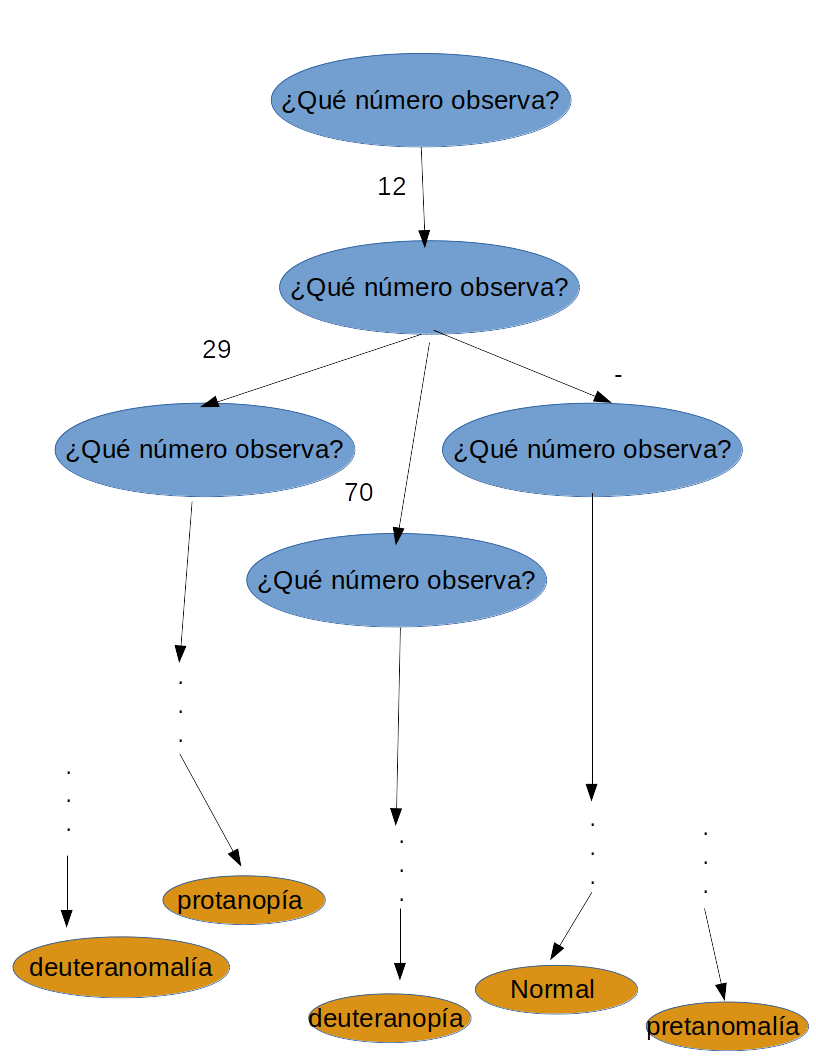
\includegraphics[scale = 0.60]{Imagenes/arbol.png}
\captionof{figure}{\label{fig:2} Ejemplo de árbol de decisiones} 
	\end{center} 
\end{figure}
\newpage
\section{Análisis}
\subsection{Viabilidad}

\subsubsection{Alcance}

Como fue definido en el planteamiento del problema, el proyecto buscará realizar un análisis para conocer que si el paciente es daltónico o no, para después transformar los colores buscando emular la manera correcta de la gama cromática.

\subsubsection{Análisis de situación}

\textbf{Fortalezas:}
\begin{itemize}
    \item Diagnosticará de manera más eficiente y sin error humano a un paciente con daltonismo.
    \item Apoyará de manera más eficaz al oftalmólogo encargado.
    \item Reducirá el tiempo que tarda en realizarse el test de ishihara.
    \item Será una manera más interactiva para el paciente, principalmente si se trata de un menor de edad.
    \item Se buscará ser empleado en sistemas de bajos recursos.
    \item Será ecológico, realizando un estudio libre de hojas de papel.
\end{itemize}


\textbf{Debilidades:}
\begin{itemize}
    \item Se tendrá que contar con equipo de cómputo, en caso de no tenerlo involucrará un costo para el oftalmólogo.
    \item Podría verse afectado si el estudio es realizado con luz artificial.
   \item  Es mas económico si es realizado de la manera clásica.
\end{itemize}

\subsubsection{Enfoque}

La herramienta se idealiza principalmente a ser siempre controlada por personal calificado, que en el caso del proyecto será el oftalmólogo, como se marcó en el planteamiento del problema, el paciente aunque no tiene un interacción directa con el sistema, se ve beneficiado debido al ser diagnosticado y apoyado a través de la herramienta.

\subsubsection{Conclusión de la viabilidad}

A pesar de que falta realizar la factibilidad económica y técnica, podemos definir que es un proyecto viable, ya que en la actualidad se cuenta con pocas herramientas que apoyen a las personas con daltonismo.

Se pueden identificar más beneficios(Fortalezas) que problemas(Debilidades) por lo cual a consideración de las factibilidades, el proyecto tiende a ser viable.

\newpage
\subsection{Factibilidad}

\subsubsection{Factibilidad Técnica}

Debido a que se trata de un sistema de muy pocos requerimientos, funcionará de manera correcta en cualquier equipo.

Se busca principalmente que el sistema funcione en cualquier computadora, debido a que este deberá ser instalado en los equipos personales y/o laborales de cualquier oftalmólogo.

El único requerimiento necesario que sea de tal calidad, es el uso de una pantalla AMOLED o superior en el uso de las gafas, debido a que este tipo de luces logran manejar los colores de manera mas ideal, sin alterar el haz de luz, que podría crear un estudio erróneo.

A continuación mostraré los requerimientos mínimos para poder instalar el sistema.


\begin{figure}[H]
	\begin{center}
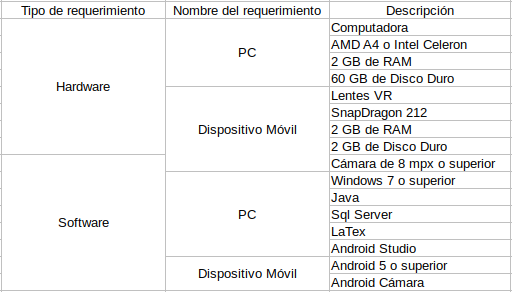
\includegraphics[scale = 0.80]{Imagenes/tabla.png}
\captionof{figure}{\label{fig:2} Tabla de factabilidad} 
	\end{center} 
\end{figure}

Dando como conclusión que se buscará sea implementado en cualquier dispositivo, ya que en el sector público no se cuenta con equipo avanzado para su ejecución.

\subsubsection{Factibilidad Económica}

En la factibilidad económica solo se contará todo aquel costo que se empleará para la creación del software, así como el hardware necesario con el que no se cuente.

\textbf{Activos}

\begin{table}[htbp]
\begin{center}
\begin{tabular}{|p{4.2cm}|p{4.2cm}|}
\hline
Activo & Costo/mes  \\
\hline
Electricidad &  30 \\
\hline
Agua &  17.50 \\
\hline
transporte &  360 \\
\hline
Internet & 700\\
\hline
Licencias & 0\\
\hline
SUBTOTAL & 117.5\\
\hline
\end{tabular}
\caption{Calculo de activos.}
\label{tabla1}
\end{center}
\end{table}

Esto nos da como resultado un total de \$ 1410 00/00 M.N. en el caso de los activos durante todo el proyecto. 

\textbf{Gastos}

\begin{table}[htbp]
\begin{center}
\begin{tabular}{|p{4.2cm}|p{4.2cm}|}
\hline
Gastos & Costo\\
\hline
Lentes VR &  200 \\
\hline
SUBTOTAL & 200\\
\hline
\end{tabular}
\caption{Calculo de Gastos.}
\label{tabla1}
\end{center}
\end{table}

Esto nos da un resultado total de \$ 200 00/00 M.N. en el caso de los gastos adicionales del proyecto. 

Debido a que los médicos en el sector público cuentan con una computadora, no se incluyen gastos en cuanto a infraestructura.

\subsection{Métricas y estimaciones}
Las métricas y estimaciones se realizarán a través de la métrica orientada a la función debido a que las tecnologías empleadas son orientadas a objetos.

\subsubsection{Métrica orientada a la función}
\begin{table}[htbp]
\begin{center}
\begin{tabular}{|p{2.2cm}|p{2.2cm}|p{2.2cm}|p{2.2cm}|}
\hline
Parámetros de medición & Factor medio & Cuenta & Resultado  \\
\hline
Número de entradas del usuario &  4 & 3 & 12\\
\hline
Número de salidas del usuario &  5 & 2 & 10\\
\hline
Número de peticiones del usuario &  4 & 2 & 8\\
\hline
Número de archivos &  10 & 2 & 20\\
\hline
Número de interfaces externas &  7 & 1 & 7\\
\hline
\end{tabular}
\caption{Métrica orientada a la función.}
\label{tabla1}
\end{center}
\end{table}

\newpage

\textbf{Preguntas:}

¿Qué necesidades de comunicación requiere el sistema para transferencia o intercambio de información? \textbf{4}

¿Existen funciones de procesamiento distribuido?  \textbf{2}

¿Es crítico el rendimiento?  \textbf{2}

¿En qué medida se está utilizando la plataforma hardware en donde se ejecutará la aplicación? \textbf{3}

¿Con qué frecuencia se ejecutan las transacciones? (diariamente, semanalmente, mensualmente, etc...)  \textbf{2}

¿Requiere el sistema entrada de datos interactiva? \textbf{4}

¿Se diseñó la aplicación pensando en que fuera eficiente y fácilmente utilizable por el usuario?  \textbf{4}

¿Cuántos ficheros Ficheros Lógicos Internos se actualizan interactivamente (por medio de transacciones on-line)? \textbf{5}

¿Existe mucha carga en cuanto a procesami. lógico y/o matemático?  \textbf{4}

¿Se desarrolló la aplicación para cumplir las necesidades de más de un usuario?  textbf{4}

¿Se ha incluido en el diseño la conversión y la instalación?  \textbf{3}

¿Requiere el sistema copias de seguridad y de recuperación fiables?  \textbf{4}

¿Se diseñó y desarrolló el sistema para soportar múltiples instalaciones en diferentes organizaciones? \textbf{2} 

¿Se diseñó y desarrolló el sistema pensando en facilitar el posterior proceso de mantenimiento? \textbf{2}

\textbf{CUENTAS}

PF=cuenta total x [0.65+0.01xE(fi)]

PF=57 x [0.65+0.55]

PF=57 x [1.2]

PF=68.4=68

Costo = \$/PF = 57/68.4 = \$0.833 por función

Calidad = errores/PF = 2/68.4 = 0.02923 errores por función

Productividad = PF/personas = 68.4/1 = 68.4 funciones por 
persona

Documentación = páginas/PF = 100/68.5 = 1.46 funciones por página

\subsubsection{COCOMO II}

\begin{figure}[H]
	\begin{center}
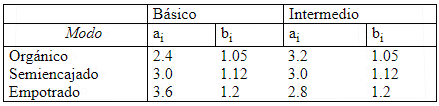
\includegraphics{Imagenes/COCOMO.PNG}
\captionof{figure}{\label{fig:2} Cuadro de COCOMO II} 
	\end{center} 
\end{figure}
Se utilizan dos ecuaciones para determinar el esfuerzo de personal y el tiempo de desarrollo. El coste es:

\begin{equiation}
E = 2.4 (S_{k})^(1.05)
\end{equiation}

donde E se expresa en personas-mes y Sk es el tamaño expresado en miles de líneas de código fuente. El tiempo de desarrollo se da por  

\begin{equiation}
D = 2.5 E^(0.38)
\end{equiation}

Donde E se obtiene de la ecuación anterior y D es el tiempo de desarrollo en meses suponiendo que no arrebase las 1500 lineas de código.
Dándonos como resultado:

E= 5.18/mes.
D= 4.6 meses de trabajo.

Deduciendo con facilidad, que el número óptimo de personas para trabajar en el proyecto son 1.12 personas, que dá un total de 1 persona.

\subsection{Mecanismos de seguimiento y control}

Scrum cuenta con una característica denominada sprint, ejecución de la iteración, que consiste en un intervalo prefijado durante el que se crea un incremento de producto utilizable. De esta manera los integrantes del proyecto reportarán sus avances periódicamente y serán tomadas medidas de consideración si hay algún problema o retraso. Seguido de ejecutar las herramientas tales como la Scrum TaskBoard y la Burndown Chart.


\subsection{Análisis de requerimientos}
\subsubsection{Historias de usuario}
La metodología \textit{Scrum} nos ofrece ya un análisis de requerimientos, este es a través de las historias de usuario, de las cuales ya se hablaron durante la definición de la métrica.

Por lo que primeramente, se ilustrarán las historias de las que se obtuvieron los requerimientos.

\begin{figure}[H]
	\begin{center}
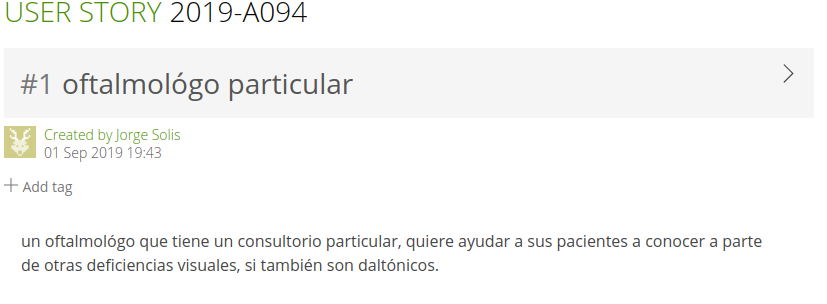
\includegraphics[scale = .55]{HS/US1.png}
\captionof{figure}{\label{fig:2} Historia de usuario 1}
	\end{center} 
\end{figure}


\begin{figure}[H]
	\begin{center}
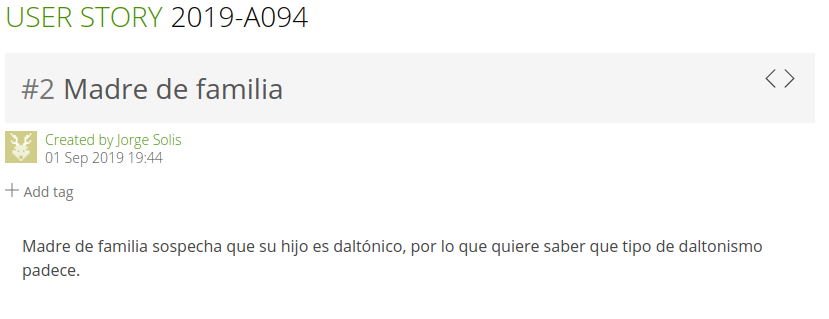
\includegraphics[scale = 0.55]{HS/US2.png}
\captionof{figure}{\label{fig:2} Historia de usuario 2}
	\end{center} 
\end{figure}

\begin{figure}[H]
	\begin{center}

\includegraphics[scale = 0.55]{HS/US3.png}
\captionof{figure}{\label{fig:2} Historia de usuario 3}
	\end{center} 
\end{figure}

\begin{figure}[H]
	\begin{center}
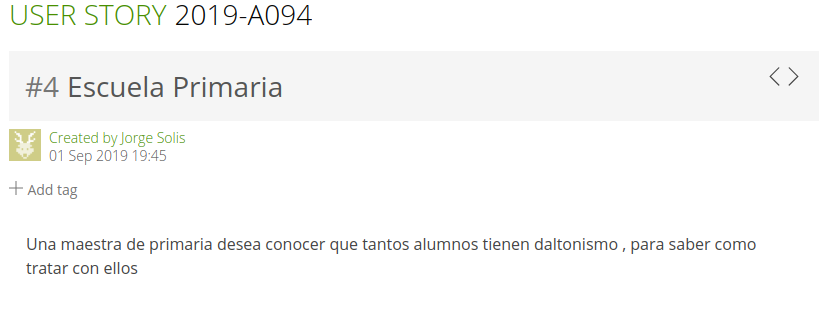
\includegraphics[scale = 0.55]{HS/US4.png}
\captionof{figure}{\label{fig:2} Historia de usuario 4}
	\end{center} 
\end{figure}

\begin{figure}[H]
	\begin{center}

\includegraphics[scale = 0.55]{HS/US5.png}
\captionof{figure}{\label{fig:2} Historia de usuario 5}
	\end{center} 
\end{figure}

Como resultado se elaboran una serie de requerimientos funcionales los cuales son:
\subsubsection{Requerimientos Funcionales}

\begin{enumerate}
    \item Debe contar con una aplicación de escritorio
    \item Los lentes deben de tener algún disposivo móvil o embebido.
    \item La aplicación debe contar con una base de datos de pacientes.
    \item La aplicación debe ser controlada todo el tiempo por la computadora.
    \item El médico debe contar con un \textit{log in} para cuestiones de seguridad de sus pacientes.
    \item Se debe digitalizar las cartas de ishihara para su proyección.
    
\end{enumerate}

\subsubsection{Requerimientos no Funcionales}

\begin{enumerate}
    \item La aplicación debe tener una interfaz libre de colores primarios.
    \item Debe contar con suficiente luz el entorno donde se realizará el diagnostico.
    \item Debe ser usada por un médico oftalmólogo.
    \item El dispositivo debe contar con una cámara.
    \item Debe contar con una interfaz intuitiva para el médico.
    
\end{enumerate}

\newpage
\subsection{Análisis de Riesgos}

\textbf{Identificación y Clasificación}

\begin{table}[htbp]
\begin{center}
\begin{tabular}{|p{2.2cm}|p{2.2cm}|p{2.2cm}|p{2.2cm}|p{2.2cm}|}
\hline
Riesgo & Categoría & Probabilidad & Impacto & Mitigación \\
\hline
Estimación baja del tamaño & PS & 30\% & 2 & Hacer una nueva estimación en cada Sprint del proyecto\\
\hline

Fecha de entrega equivocada & BU & 20\% & 2 & Seguir y controlar apropiadamente el proyecto en cada sprint. \\
\hline
Perdida de fondos & CU & 5\% & 1 & Seguir y controlar apropiadamente el gasto en cada sprint, realizar la retrospectiva debida del sprint. \\
\hline
Tecnología no santisface las expectativas & TE & 40\% & 3 & Mantener las herramientas de desarrollo actualizadas. \\
\hline
Ocurre alguna enfermedad que incapacite a algún director o a mí & CU & 70\% & 5 & Generar una ruta critica del sprint dependiendo del tiempo en el que alguno de los integrantes se vea incapacitado. \\
\hline
Falta de servicio de luz & CU & 30\% & 2 & Generar una ruta critica para no sobrepasar el tiempo límite. \\
\hline
\end{tabular}
%\caption{Identificación y Clasificación.}
\label{tabla2}
\end{center}
\end{table}

\begin{table}[htbp]
\begin{center}
\begin{tabular}{|p{2.2cm}|p{2.2cm}|p{2.2cm}|p{2.2cm}|p{2.2cm}|}
\hline
Falta de servicio de internet & CU & 30\% & 2 & Generar una ruta critica para no sobrepasar el tiempo límite. \\
\hline
Perdida de equipo de computo & TE & 70\% & 4 & Mantener la información actualizada en una nube segura, como copia de seguridad y contar con una computadora que sirva de \textit{backup}. \\
\hline
Perdida de información & TE & 70\% & 4 & Mantener la información actualizada en una nube segura, como copia de seguridad. \\
\hline
Sinodal no se presenta a presentación &CU & 70\% & 4 & Seguir el protocolo de la CATT, y esperar a la decisión consensuada entre los directores y los sinodales asistentes, para poder generar el quórum necesario. \\
\hline
Correcciones en documentación  & BU & 50\% & 3 & Generar una ruta critica con las correcciones pertinentes que no hagan un impacto en los siguientes Sprint. \\
\hline
Encontrar una tarea no indentificada en el análisis & TE & 30\% & 2 & Scrum mitiga el riesgo, presentando la oportunidad de corregir un sprint. \\
\hline
\end{tabular}
\caption{Identificación y Clasificación.}
\label{tabla2}
\end{center}
\end{table}



\newpage

\section{Diseño}

\subsection{Diagrama de arquitectura del sistema}

Este diagrama refleja lo que será, en cuanto a procesos, la herramienta que se realizará.

\begin{figure}[H]
	\begin{center}
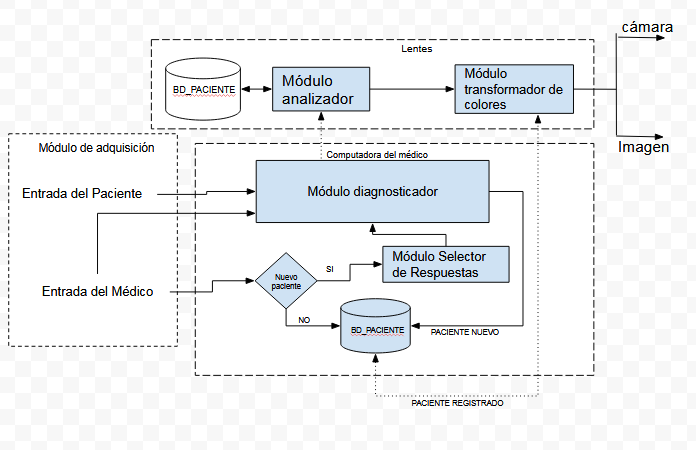
\includegraphics[scale = 0.75]{Imagenes/BOSQUEJO.PNG}
\captionof{figure}{\label{fig:2} Diagrama a alto nivel de la herramienta}
	\end{center} 
\end{figure}


\subsection{UML}
Para el diseño, se comenzó con los diagramas UML ya que se optó por realizar un software que siga el paradigma orientado a objetos, con el que podrá funcionar de manera eficiente.

Estos son los diagramas UML que se consideran necesarios para lograr la implementación del proyecto:

\begin{itemize}
    \item Diagrama de casos de uso.
    \item Diagrama de Clases.
    \item Diagrama de estados.
    \item Diagrama de secuencias.
    \item Diagrama de actividades. 
    \item Diagrama de componentes.
\end{itemize}

A continuación los observaremos dando una breve explicación de los mismos.

\newpage

\subsubsection{Diagrama de casos de uso}

El diagrama de casos es el más fundamental en cada sistema y en este proyecto ayudará para conocer más a fondo algunos aspectos del sistema.

\begin{figure}[H]
	\begin{center}
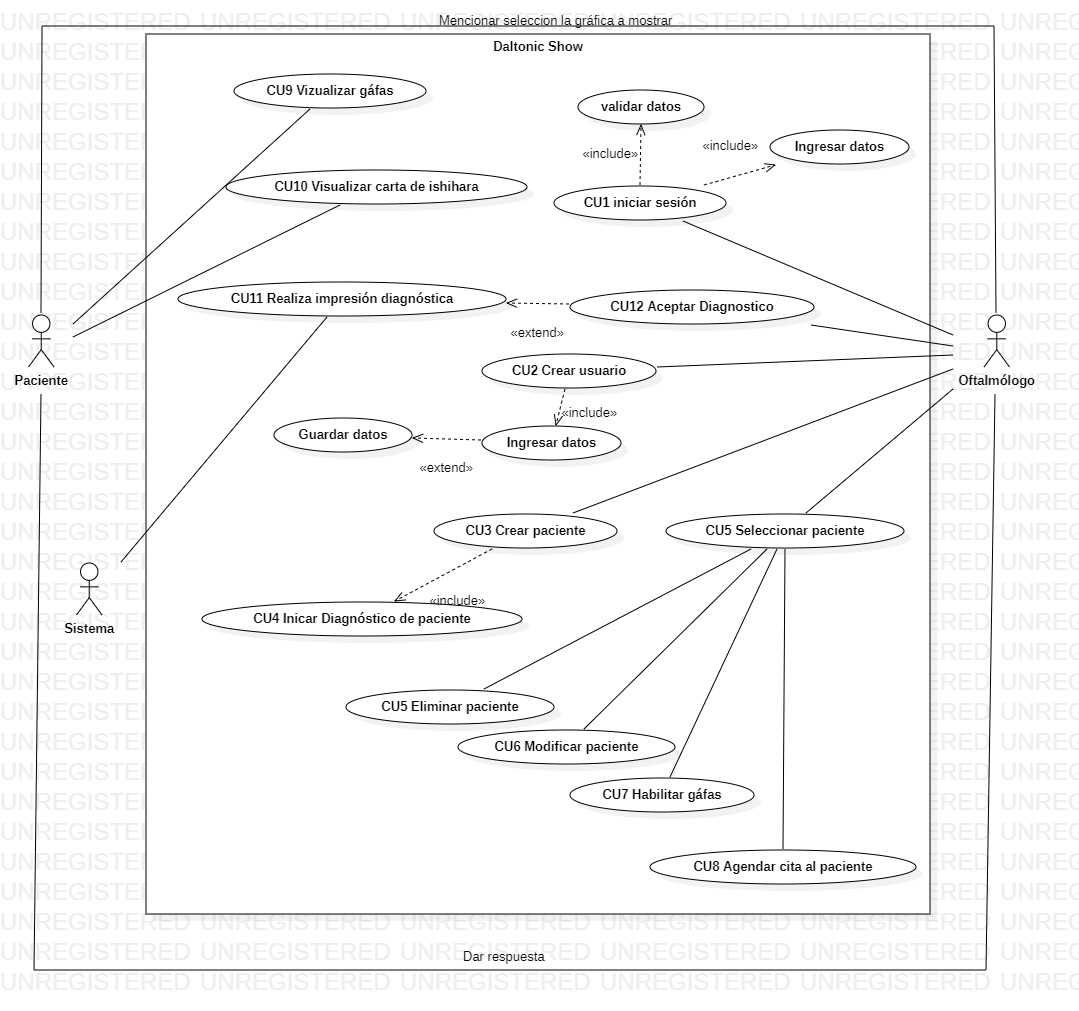
\includegraphics[scale = 0.40]{UML/UseCaseDiagram1.jpg}
\captionof{figure}{\label{fig:2} Diagrama de casos de uso}
	\end{center} 
\end{figure}

\newpage


\subsubsection{Tablas de mensajes}

\begin{longtable}{|p{5.0cm}|p{3.5cm}|p{6.5cm}|}
\hline
Tabla de mensajes\\
\hline 
\endfirsthead

% aquí añadimos el encabezado del resto de hojas.
\hline

Tabla de mensajes\\
\hline 
\endhead

% aquí añadimos el fondo de todas las hojas, excepto de la última.
\multicolumn{3}{c}{}
\endfoot

% aquí añadimos el fondo de la última hoja.
\endlastfoot
\hline
ID & Tipo & Descripción\\
\hline

msj1 & Mensaje de entrada & El mensaje sirve para que el oftalmólogo pueda introducir la cadena del usuario para ser validada por el software a través de los registros encontrados en la base de datos.\\
\hline

msj2 & Mensaje de entrada & El mensaje sirve para que el oftalmólogo pueda introducir la cadena de contraseña para ser validado por el software a través de los registros encontrados en la base de datos.\\
\hline

msj3 & Mensaje de salida & Le indica al oftalmólogo que fue exitosa su entrada del usuario y contraseña introducidos con anterioridad en el diseño. \\
\hline

msj4 & Mensaje de error & Le indica al oftalmólogo que no fue exitosa su entrada de usuario y contraseña introducidos con anterioridad en el diseño\\
\hline

msj5 & Mensaje de opción & Le pregunta al oftalmólogo si desea cerrar la sesión actual, en caso de decir que no, se mantendrá la sesión, en caso de cerrar, se olvidarán los datos de la sesión.\\
\hline

msj6 & Mensaje de opción & Le pregunta al oftalmólogo si desea entrar a las gafas del paciente en modo cámara o imagen \\
\hline

msj7 & Mensaje de advertencia & Le pregunta al oftalmólogo si realmente desea salir del software y cerrarlo definitivamente \\
\hline

msj8 & Mensaje de salida & Muestra el mensaje del aviso de privacidad \\
\hline

msj9 & Mensaje de salida & Muestra el quien lo desarrollo y los directores del trabajo terminal \\
\hline

msj10 & Mensaje de Error & Muestra el error al generar un usuario o paciente \\
\hline

msj11 & Mensaje de Error &  Muestra el error al ingresar un dato en la generación de usuario o paciente\\
\hline

msj12 & Mensaje de salida & Menciona que se creó el usuario correctamente \\
\hline

msj13 & Mensaje de Error & Menciona el error al crear una cita en la agenda \\
\hline
msj14 & Mensaje de salida & Muestra que se generó correctamente la cita del paciente \\
\hline
msj15 & Mensaje de salida & Avisa al oftalmólogo el inicio del diagnóstico.\\
\hline
msj16 & Mensaje de salida & Muestra al oftalmólogo el tipo de daltonismo que padece el paciente. \\
\hline
\caption{Tabla de mensajes}
\label{tabla1}
\end{longtable}

\newpage

\subsubsection{Tablas de casos de uso}
\begin{longtable}{|p{3.8cm}|p{10.8cm}|}
\hline
CASO DE USO & CU1: Iniciar sesión\\
\hline 
\endfirsthead

% aquí añadimos el encabezado del resto de hojas.
\hline

CASO DE USO & CU1: Iniciar sesión\\
\hline 
\endhead

% aquí añadimos el fondo de todas las hojas, excepto de la última.
\multicolumn{2}{c}{}
\endfoot

% aquí añadimos el fondo de la última hoja.
\endlastfoot
\hline
versión & 1\\
\hline
Autor & Jorge Armando Solis Solis\\
\hline
Revisiones & Gabriela de Jesús López Ruiz\newline
José Carlos Davalos López\newline
Edgar Armando Catalán Salgado\newline
Rafael Norman Delgado Saucedo\newline
Rosa Itzel Solis Solis
\\

\hline
Fecha de última revisión & 26/02/20\\
\hline
Actor(es) & Oftalmólogo \\
\hline
Propósito & El oftalmólogo debe de iniciar sesión para poder comprobar que se trata de él, debido a la información sensible que maneja el sistema.\\
\hline
Entradas & usuario y contraseña\\
\hline
salidas & mensaje de inicio de sesión exitoso\\
\hline
Mensajes & ms1, ms2, msj3 msj4\\
\hline
Pre-condiciones & haber creado un usuario \\
\hline
Post-condiciones &  encontrar usuario y contraseña correctos \\
\hline
Flujo principal & \begin{enumerate}
    \item El oftalmólogo ingresa usuario.
    \item El oftalmólogo ingresa contraseña.
    \item El oftalmólogo da en el botón aceptar.
    \item El sistema valida datos en la base de datos.
    \item El sistema despliega el mensaje de éxito.
\end{enumerate}
    \\
\hline
Flujos Alternos &  \begin{enumerate}
    \item El oftalmólogo ingresa usuario.
    \item El oftalmólogo ingresa contraseña.
    \item El oftalmólogo da en el botón aceptar.
    \item El sistema valida datos en la base de datos.
    \item El sistema no encuentra datos.
    \item el sistema despliega mensaje de error.
    \item El oftalmólogo reingresa los datos.
\end{enumerate}\\
\hline
\caption{CASO DE USO 1}
\label{tabla1}
\end{longtable}

\newpage

\begin{longtable}{|p{3.8cm}|p{10.8cm}|}
\hline
CASO DE USO & CU2: Crear usuario\\
\hline 
\endfirsthead

% aquí añadimos el encabezado del resto de hojas.
\hline

CASO DE USO & CU2: Crear usuario\\
\hline 
\endhead

% aquí añadimos el fondo de todas las hojas, excepto de la última.
\multicolumn{2}{c}{}
\endfoot

% aquí añadimos el fondo de la última hoja.
\endlastfoot
\hline
versión & 1\\
\hline
Autor & Jorge Armando Solis Solis\\
\hline
Revisiones & Gabriela de Jesús López Ruiz\newline
José Carlos Davalos López\newline
Edgar Armando Catalán Salgado\newline
Rafael Norman Delgado Saucedo\newline
Rosa Itzel Solis Solis
\\

\hline
Fecha de última revisión & 26/02/20\\
\hline
Actor(es) & Oftalmólogo \\
\hline
Propósito & El oftalmólogo desea crear un usuario no existente en la base de datos, para poder visualizar los pacientes.\\
\hline
Entradas & Nombre, apellido, cédula profesional, usuario, contraseña\\
\hline
salidas & mensaje de inicio creación de usuario\\
\hline
Mensajes & ms10, ms11, msj12\\
\hline
Pre-condiciones & Ser un oftalmólogo interesado en crear un usuario \\
\hline
Post-condiciones & usuario validado y guardado en la base de datos con la información proporcionada. \\
\hline
Flujo principal & \begin{enumerate}
    \item El oftalmólogo entra a la opción crear usuario.
    \item Ingresar los datos de entrada.
    \item El oftalmólogo da en el botón aceptar.
    \item El sistema valida datos y los ingresa en la base de datos.
    \item El sistema despliega el mensaje de éxito.
\end{enumerate}
    \\
\hline
Flujos Alternos &  \begin{enumerate}
    \item El oftalmólogo entra a la opción crear usuario.
    \item Ingresar los datos de entrada.
    \item El oftalmólogo da en el botón aceptar.
    \item El sistema valida datos.
    \item El sistema encuentra un error en los datos.
    \item El sistema encuentra solicita el dato incorrecto.
    \item El oftalmólogo ingresa el dato corregido.
    \item El oftalmólogo valida e ingresa los datos.
    \item El sistema despliega el mensaje de éxito.
\end{enumerate}\\
\hline
\caption{CASO DE USO 2}
\label{tabla1}
\end{longtable}

\newpage

\begin{longtable}{|p{3.8cm}|p{10.8cm}|}
\hline
CASO DE USO & CU3: Crear paciente\\
\hline 
\endfirsthead

% aquí añadimos el encabezado del resto de hojas.
\hline

CASO DE USO & CU2: Crear paciente\\
\hline 
\endhead

% aquí añadimos el fondo de todas las hojas, excepto de la última.
\multicolumn{2}{c}{}
\endfoot

% aquí añadimos el fondo de la última hoja.
\endlastfoot
\hline
versión & 1\\
\hline
Autor & Jorge Armando Solis Solis\\
\hline
Revisiones & Gabriela de Jesús López Ruiz\newline
José Carlos Davalos López\newline
Edgar Armando Catalán Salgado\newline
Rafael Norman Delgado Saucedo\newline
Rosa Itzel Solis Solis
\\

\hline
Fecha de última revisión & 26/02/20\\
\hline
Actor(es) & Oftalmólogo \\
\hline
Propósito & El oftalmólogo recibe un nuevo paciente, debe guardarlo en la base de datos para proceder a diagnosticarlo. \\
\hline
Entradas & Nombre, apellido, fecha de ingreso, fecha de nacimiento.\\
\hline
salidas & mensaje de inicio creación de usuario\\
\hline
Mensajes & ms10, ms11, msj12\\
\hline
Pre-condiciones & Paciente nuevo desea realizarse estudio del daltonismo.\\
\hline
Post-condiciones & El paciente debe realizar el diagnóstico.\\
\hline
Flujo principal & \begin{enumerate}
    \item El oftalmólogo entra a la opción crear nuevo paciente.
    \item Ingresar los datos de entrada.
    \item El oftalmólogo da en el botón aceptar.
    \item El sistema valida datos y los ingresa en la base de datos.
    \item El sistema despliega el mensaje de éxito.
    \item Comienza el diagnóstico. 
\end{enumerate}
    \\
\hline
Flujos Alternos &  \begin{enumerate}
    \item El oftalmólogo entra a la opción crear nuevo.
    \item Ingresar los datos de entrada.
    \item El oftalmólogo da en el botón aceptar.
    \item El sistema valida datos.
    \item El sistema encuentra un error en los datos.
    \item El sistema encuentra solicita el dato incorrecto.
    \item El oftalmólogo ingresa el dato corregido.
    \item El oftalmólogo valida e ingresa los datos.
    \item El sistema despliega el mensaje de éxito.
    \item Comienza el diagnóstico.
\end{enumerate}\\
\hline
\caption{CASO DE USO 3}
\label{tabla1}
\end{longtable}

\newpage

\begin{longtable}{|p{3.8cm}|p{10.8cm}|}
\hline
CASO DE USO & CU4: Iniciar diagnóstico del paciente\\
\hline 
\endfirsthead

% aquí añadimos el encabezado del resto de hojas.
\hline

CASO DE USO & CU4: Iniciar diagnóstico del paciente\\
\hline 
\endhead

% aquí añadimos el fondo de todas las hojas, excepto de la última.
\multicolumn{2}{c}{}
\endfoot

% aquí añadimos el fondo de la última hoja.
\endlastfoot
\hline
versión & 1\\
\hline
Autor & Jorge Armando Solis Solis\\
\hline
Revisiones & Gabriela de Jesús López Ruiz\newline
José Carlos Davalos López\newline
Edgar Armando Catalán Salgado\newline
Rafael Norman Delgado Saucedo\newline
Rosa Itzel Solis Solis
\\

\hline
Fecha de última revisión & 26/02/20\\
\hline
Actor(es) & Oftalmólogo \\
\hline
Propósito & El oftalmólogo recibe un nuevo paciente, después de ingresarlo en su base de datos, desea diagnosticarlo. \\
\hline
Entradas & Paciente a diagnosticar, datos que visualiza el paciente.\\
\hline
salidas & Cartas de ishihara, tipo de daltonismo que padece. \\
\hline
Mensajes & ms15, ms16\\
\hline
Pre-condiciones & Paciente nuevo desea realizarse estudio del daltonismo\\
\hline
Post-condiciones & Paciente tiene un tipo de daltonismo.\\
\hline
Flujo principal & \begin{enumerate}
    \item El oftalmólogo pulsa el botón de diagnosticar.
    \item El sistema muestra la carta de ishihara correspondiente.
    \item El paciente menciona el dato que visualiza.
    \item El oftalmólogo ingresa el valor mencionado por el paciente.
    \item El sistema realiza la impresión diagnóstica.
    \item El oftalmólogo acepta el diagnóstico.
    \item El paciente padece algún tipo de daltonismo.
    \item El sistema almacena en la base de datos el tipo de daltonismo.
    \item Al paciente se le habilita la opción de habilitar gafas.
\end{enumerate}
    \\
\hline
Flujos Alternos &  \begin{enumerate}
    \item El oftalmólogo pulsa el botón de diagnosticar.
    \item El sistema muestra la carta de ishihara correspondiente.
    \item El paciente menciona el dato que visualiza.
    \item El oftalmólogo ingresa el valor mencionado por el paciente.
    \item El sistema realiza la impresión diagnóstica.
    \item El oftalmólogo acepta el diagnóstico.
    \item El paciente no padece algún tipo de daltonismo.
    \item El sistema almacena en la base de datos el tipo de daltonismo.
\end{enumerate}\\
\hline
\caption{CASO DE USO 4}
\label{tabla1}
\end{longtable}

\newpage

\begin{longtable}{|p{3.8cm}|p{10.8cm}|}
\hline
CASO DE USO & CU5: Seleccionar paciente\\
\hline 
\endfirsthead

% aquí añadimos el encabezado del resto de hojas.
\hline

CASO DE USO & CU5: Seleccionar paciente\\
\hline 
\endhead

% aquí añadimos el fondo de todas las hojas, excepto de la última.
\multicolumn{2}{c}{}
\endfoot

% aquí añadimos el fondo de la última hoja.
\endlastfoot
\hline
versión & 1\\
\hline
Autor & Jorge Armando Solis Solis\\
\hline
Revisiones & Gabriela de Jesús López Ruiz\newline
José Carlos Davalos López\newline
Edgar Armando Catalán Salgado\newline
Rafael Norman Delgado Saucedo\newline
Rosa Itzel Solis Solis
\\

\hline
Fecha de última revisión & 26/02/20\\
\hline
Actor(es) & Oftalmólogo \\
\hline
Propósito & El oftalmólogo recibe un paciente, lo busca en la base de datos. \\
\hline
Entradas & Paciente encontrado en base de datos\\
\hline
salidas & Cartas de ishihara, tipo de daltonismo que padece. \\
\hline
Mensajes & \\
\hline
Pre-condiciones & Paciente debe de estar registrado previamente.\\
\hline
Post-condiciones & Paciente tiene un tipo de daltonismo.\\
\hline
Flujo principal & \begin{enumerate}
    \item El oftalmólogo pulsa el botón de seleccionar paciente.
    \item El sistema muestra los pacientes posibles registrados a seleccionar.
    \item El oftalmólogo selecciona el paciente.
    \item El sistema despliega la información del paciente y las funciones posibles.
\end{enumerate}
    \\
\hline
Flujos Alternos &  \begin{enumerate}
    \item El oftalmólogo pulsa el botón de seleccionar paciente.
    \item El sistema muestra los pacientes posibles registrados a seleccionar.
    \item El paciente no está en la base de datos. 
    \item El oftalmólogo crea y diagnóstica al paciente.
    \item El oftalmólogo pulsa el botón seleccionar paciente.
    \item El oftalmólogo selecciona el paciente.
    \item El paciente despliega la información del paciente y las funciones posibles.
\end{enumerate}\\
\hline
\caption{CASO DE USO 5}
\label{tabla1}
\end{longtable}

\newpage

\begin{longtable}{|p{3.8cm}|p{10.8cm}|}
\hline
CASO DE USO & CU6: Eliminar paciente\\
\hline 
\endfirsthead

% aquí añadimos el encabezado del resto de hojas.
\hline

CASO DE USO & CU6: Eliminar paciente\\
\hline 
\endhead

% aquí añadimos el fondo de todas las hojas, excepto de la última.
\multicolumn{2}{c}{}
\endfoot

% aquí añadimos el fondo de la última hoja.
\endlastfoot
\hline
versión & 1\\
\hline
Autor & Jorge Armando Solis Solis\\
\hline
Revisiones & Gabriela de Jesús López Ruiz\newline
José Carlos Davalos López\newline
Edgar Armando Catalán Salgado\newline
Rafael Norman Delgado Saucedo\newline
Rosa Itzel Solis Solis
\\

\hline
Fecha de última revisión & 26/02/20\\
\hline
Actor(es) & Oftalmólogo \\
\hline
Propósito & El oftalmólogo por alguna razón desea eliminar a un paciente. \\
\hline
Entradas & Paciente se encuentra en base de datos y ha sido seleccionado\\
\hline
salidas & El paciente ha sido eliminado. \\
\hline
Mensajes & ms12\\
\hline
Pre-condiciones & Paciente debe de estar registrado previamente.\\
\hline
Post-condiciones & Paciente no debe de estar registrado en base de datos.\\
\hline
Flujo principal & \begin{enumerate}
    \item El oftalmólogo pulsa el botón eliminar paciente.
    \item El sistema elimina de la base de datos al paciente.
    \item El sistema lanza el mensaje de paciente eliminado.
    
\end{enumerate}
    \\
\hline
Flujos Alternos &  
    N/A\\
\hline
\caption{CASO DE USO 6}
\label{tabla1}
\end{longtable}


\begin{longtable}{|p{3.8cm}|p{10.8cm}|}
\hline
CASO DE USO & CU7: Habilitar gafas\\
\hline 
\endfirsthead

% aquí añadimos el encabezado del resto de hojas.
\hline

CASO DE USO & CU7: Habilitar gafas\\
\hline 
\endhead

% aquí añadimos el fondo de todas las hojas, excepto de la última.
\multicolumn{2}{c}{}
\endfoot

% aquí añadimos el fondo de la última hoja.
\endlastfoot
\hline
versión & 1\\
\hline
Autor & Jorge Armando Solis Solis\\
\hline
Revisiones & Gabriela de Jesús López Ruiz\newline
José Carlos Davalos López\newline
Edgar Armando Catalán Salgado\newline
Rafael Norman Delgado Saucedo\newline
Rosa Itzel Solis Solis
\\

\hline
Fecha de última revisión & 26/02/20\\
\hline
Actor(es) & Oftalmólogo \\
\hline
Propósito & El oftalmólogo habilita gafas con la imagen en colores cercanos a la visión normal para el paciente.\\
\hline
Entradas & Selección del paciente, paciente diagnosticado.\\
\hline
salidas & imagen en colores cercanos a la visión normal.\\
\hline
Mensajes & \\
\hline
Pre-condiciones & El paciente debe estar registrado.\\
\hline
Post-condiciones & El paciente debe de tener los datos actualizados en la base.\\
\hline
Flujo principal & \begin{enumerate}
    \item El oftalmólogo pulsa el botón habilitar gafas.
    \item El paciente visualiza la imagen.
\end{enumerate}
    \\
\hline
Flujos Alternos &  N/A\\
\hline
\caption{CASO DE USO 7}
\label{tabla1}
\end{longtable}

\newpage 
\begin{longtable}{|p{3.8cm}|p{10.8cm}|}
\hline
CASO DE USO & CU8: Modificar paciente\\
\hline 
\endfirsthead

% aquí añadimos el encabezado del resto de hojas.
\hline

CASO DE USO & CU8: Modificar paciente\\
\hline 
\endhead

% aquí añadimos el fondo de todas las hojas, excepto de la última.
\multicolumn{2}{c}{}
\endfoot

% aquí añadimos el fondo de la última hoja.
\endlastfoot
\hline
versión & 1\\
\hline
Autor & Jorge Armando Solis Solis\\
\hline
Revisiones & Gabriela de Jesús López Ruiz\newline
José Carlos Davalos López\newline
Edgar Armando Catalán Salgado\newline
Rafael Norman Delgado Saucedo\newline
Rosa Itzel Solis Solis
\\

\hline
Fecha de última revisión & 26/02/20\\
\hline
Actor(es) & Oftalmólogo \\
\hline
Propósito & El oftalmólogo desea modificar los datos del paciente por alguna razón.\\
\hline
Entradas & Datos del paciente.\\
\hline
salidas & Se actualizan los datos en la base de datos del paciente. \\
\hline
Mensajes & m13,m14\\
\hline
Pre-condiciones & El paciente debe estar registrado.\\
\hline
Post-condiciones & El paciente debe de tener los datos actualizados en la base.\\
\hline
Flujo principal & \begin{enumerate}
    \item El oftalmólogo pulsa el botón modificar paciente.
    \item El oftalmólogo ingresa los datos a modificar.
    \item El oftalmólogo pulsa aceptar paciente.
    \item El sistema acepta los cambios y los actualiza.
    
\end{enumerate}
    \\
\hline
Flujos Alternos &  \begin{enumerate}
    \item El oftalmólogo pulsa el botón modificar paciente.
    \item El oftalmólogo ingresa los datos a modificar.
    \item El oftalmólogo pulsa aceptar paciente.
    \item El sistema encuentra un error en los datos.
    \item El sistema imprime el mensaje de error.
    \item El oftalmólogo corrige los datos.
    \item El oftalmólogo valida y actualiza los datos.
\end{enumerate}
    \\
\hline
\caption{CASO DE USO 8}
\label{tabla1}
\end{longtable}


\newpage 

\begin{longtable}{|p{3.8cm}|p{10.8cm}|}
\hline
CASO DE USO & CU9: Agendar cita a paciente\\
\hline 
\endfirsthead

% aquí añadimos el encabezado del resto de hojas.
\hline

CASO DE USO & CU9: Agendar cita a paciente\\
\hline 
\endhead

% aquí añadimos el fondo de todas las hojas, excepto de la última.
\multicolumn{2}{c}{}
\endfoot

% aquí añadimos el fondo de la última hoja.
\endlastfoot
\hline
versión & 1\\
\hline
Autor & Jorge Armando Solis Solis\\
\hline
Revisiones & Gabriela de Jesús López Ruiz\newline
José Carlos Davalos López\newline
Edgar Armando Catalán Salgado\newline
Rafael Norman Delgado Saucedo\newline
Rosa Itzel Solis Solis
\\

\hline
Fecha de última revisión & 26/02/20\\
\hline
Actor(es) & Oftalmólogo \\
\hline
Propósito & EL paciente desea volver a asistir con el oftalmólogo.\\
\hline
Entradas & paciente registrado, diagnosticado y con anteriores citas.\\
\hline
salidas & Se agenda cita en fechas próximas del paciente.\\
\hline
Mensajes & m14\\
\hline
Pre-condiciones & El paciente debe estar registrado, diagnosticado y tener citas anteriores.\\
\hline
Post-condiciones & La cita se agendará en la base de datos.\\
\hline
Flujo principal & \begin{enumerate}
    \item El oftalmólogo pulsa el botón agendar paciente.
    \item El oftalmólogo ingresa los datos de la próxima cita.
    \item El oftalmólogo pulsa aceptar.
    \item El sistema valida si la fecha es valida.
    \item El sistema almacena la fecha en la base de datos.
    
\end{enumerate}
    \\
\hline
Flujos Alternos & \begin{enumerate}
    \item El oftalmólogo pulsa el botón agendar paciente.
    \item El oftalmólogo ingresa los datos de la próxima cita.
    \item El oftalmólogo pulsa aceptar.
    \item El sistema valida si la fecha es valida.
    \item El sistema imprime el mensaje de error.
    \item El oftalmólogo vuelve a ingresar la fecha.
    \item El sistema almacena la fecha en la base de datos.
\end{enumerate}
    \\
\hline
\caption{CASO DE USO 9}
\label{tabla1}
\end{longtable}

\newpage 

\begin{longtable}{|p{3.8cm}|p{10.8cm}|}
\hline
CASO DE USO & CU10: Visualizar gafas\\
\hline 
\endfirsthead

% aquí añadimos el encabezado del resto de hojas.
\hline

CASO DE USO & CU10: Visualizar gafas\\
\hline 
\endhead

% aquí añadimos el fondo de todas las hojas, excepto de la última.
\multicolumn{2}{c}{}
\endfoot

% aquí añadimos el fondo de la última hoja.
\endlastfoot
\hline
versión & 1\\
\hline
Autor & Jorge Armando Solis Solis\\
\hline
Revisiones & Gabriela de Jesús López Ruiz\newline
José Carlos Davalos López\newline
Edgar Armando Catalán Salgado\newline
Rafael Norman Delgado Saucedo\newline
Rosa Itzel Solis Solis
\\

\hline
Fecha de última revisión & 26/02/20\\
\hline
Actor(es) & paciente \\
\hline
Propósito & El paciente visualiza la imagen que seleccionó en las gafas.\\
\hline
Entradas & tipo de daltonismo que padece el paciente, selección del paciente.\\
\hline
salidas & Imagen modificada con la visión del tipo de daltonismo del paciente.\\
\hline
Mensajes & \\
\hline
Pre-condiciones & El paciente debe de estar registrado y padecer algún tipo de daltonismo.\\
\hline
Post-condiciones & N/A\\
\hline
Flujo principal & \begin{enumerate}
    \item El paciente selecciona imagen.
    \item El oftalmólogo habilita las gafas con la imagen deseada.
    \item El paciente ve imagen.
\end{enumerate}
    \\
\hline
Flujos Alternos & 
    N/A\\
\hline
\caption{CASO DE USO 10}
\label{tabla1}
\end{longtable}

\newpage 

\begin{longtable}{|p{3.8cm}|p{10.8cm}|}
\hline
CASO DE USO & CU11: Visualizar carta de ishihara\\
\hline 
\endfirsthead

% aquí añadimos el encabezado del resto de hojas.
\hline

CASO DE USO & CU11: Visualizar carta de ishihara\\
\hline 
\endhead

% aquí añadimos el fondo de todas las hojas, excepto de la última.
\multicolumn{2}{c}{}
\endfoot

% aquí añadimos el fondo de la última hoja.
\endlastfoot
\hline
versión & 1\\
\hline
Autor & Jorge Armando Solis Solis\\
\hline
Revisiones & Gabriela de Jesús López Ruiz\newline
José Carlos Davalos López\newline
Edgar Armando Catalán Salgado\newline
Rafael Norman Delgado Saucedo\newline
Rosa Itzel Solis Solis
\\

\hline
Fecha de última revisión & 26/02/20\\
\hline
Actor(es) & Paciente\\
\hline
Propósito & El paciente visualiza las cartas de ishihara que servirán al sistema para encontrar si padece daltonismo.\\
\hline
Entradas & Dato que percibe el paciente.\\
\hline
salidas & Carta de ishihara.\\
\hline
Mensajes & \\
\hline
Pre-condiciones & El paciente debe de estar registrado.\\
\hline
Post-condiciones & El paciente debe obtener el tipo de daltonismo que padece.\\
\hline
Flujo principal & \begin{enumerate}
    \item El paciente observa carta de ishihara.
    \item El paciente menciona el número que observa.
    \item El oftalmólogo lo registra.
    \item El sistema muestra la siguiente imagen.
\end{enumerate}
    \\
\hline
Flujos Alternos & 
    N/A\\
\hline
\caption{CASO DE USO 11}
\label{tabla1}
\end{longtable}

\newpage 

\begin{longtable}{|p{3.8cm}|p{10.8cm}|}
\hline
CASO DE USO & CU12: Realiza impresión diagnóstica.\\
\hline 
\endfirsthead

% aquí añadimos el encabezado del resto de hojas.
\hline

CASO DE USO & CU12: Realiza impresión diagnóstica\\
\hline 
\endhead

% aquí añadimos el fondo de todas las hojas, excepto de la última.
\multicolumn{2}{c}{}
\endfoot

% aquí añadimos el fondo de la última hoja.
\endlastfoot
\hline
versión & 1\\
\hline
Autor & Jorge Armando Solis Solis\\
\hline
Revisiones & Gabriela de Jesús López Ruiz\newline
José Carlos Davalos López\newline
Edgar Armando Catalán Salgado\newline
Rafael Norman Delgado Saucedo\newline
Rosa Itzel Solis Solis
\\

\hline
Fecha de última revisión & 26/02/20\\
\hline
Actor(es) & sistema\\
\hline
Propósito & El sistema realizará la impresión diagnóstica del paciente con base en las respuestas del paciente.\\
\hline
Entradas & Respuestas del paciente.\\
\hline
salidas & Impresión diagnóstica\\
\hline
Mensajes & \\
\hline
Pre-condiciones & El paciente debe estar registrado.\\
\hline
Post-condiciones & El paciente debe obtener el tipo de daltonismo que padece.\\
\hline
Flujo principal & \begin{enumerate}
    \item El oftalmólogo ingresa la respuesta del paciente.
    \item El sistema guarda el dato en la base.
    \item El sistema procesa la respuesta.
    \item El sistema elige si cuenta con los datos necesarios para dar la impresión diagnóstica o realiza una pregunta más.
    \item El sistema muestra la impresión diagnóstica.
\end{enumerate}
    \\
\hline
Flujos Alternos & 
    N/A\\
\hline
\caption{CASO DE USO 12}
\label{tabla1}
\end{longtable}

\newpage 

\begin{longtable}{|p{3.8cm}|p{10.8cm}|}
\hline
CASO DE USO & CU13: Aceptar diagnóstico.\\
\hline 
\endfirsthead

% aquí añadimos el encabezado del resto de hojas.
\hline

CASO DE USO & CU13: Aceptar diagnóstico.\\
\hline 
\endhead

% aquí añadimos el fondo de todas las hojas, excepto de la última.
\multicolumn{2}{c}{}
\endfoot

% aquí añadimos el fondo de la última hoja.
\endlastfoot
\hline
versión & 1\\
\hline
Autor & Jorge Armando Solis Solis\\
\hline
Revisiones & Gabriela de Jesús López Ruiz\newline
José Carlos Davalos López\newline
Edgar Armando Catalán Salgado\newline
Rafael Norman Delgado Saucedo\newline
Rosa Itzel Solis Solis
\\

\hline
Fecha de última revisión & 26/02/20\\
\hline
Actor(es) & sistema, oftalmólogo\\
\hline
Propósito & El sistema realizará la impresión diagnóstica del paciente con base en las respuestas del paciente y el oftalmólogo revelará si está en lo correcto.\\
\hline
Entradas & Impresión diagnóstica.\\
\hline
salidas & Diagnóstico.\\
\hline
Mensajes & \\
\hline
Pre-condiciones & El paciente debió haber realizado el test.\\
\hline
Post-condiciones & El paciente debe obtener el tipo de daltonismo que padece.\\
\hline
Flujo principal & \begin{enumerate}
    \item El sistema imprime la impresión diagnóstica.
    \item El oftalmólogo decide si es correcta.
    \item El oftalmólogo la acepta.
    \item El sistema la almacena en la base de datos.
\end{enumerate}
    \\
\hline
Flujos Alternos & 
    \begin{enumerate}
    \item El sistema imprime la impresión diagnóstica.
    \item El oftalmólogo decide si es correcta.
    \item El oftalmólogo no la acepta.
    \item El oftalmólogo elige el tipo de daltonismo que debería ser.
    \item El sistema lo guarda en la base de datos.
\end{enumerate}
    \\
\hline
\caption{CASO DE USO 13}
\label{tabla1}
\end{longtable}

\newpage 
\subsubsection{Diagrama de clases}


Este diagrama se diseña a partir de los casos de uso, siendo uno de los fundamentales en todo sistema.

\begin{figure}[H]
	\begin{center}
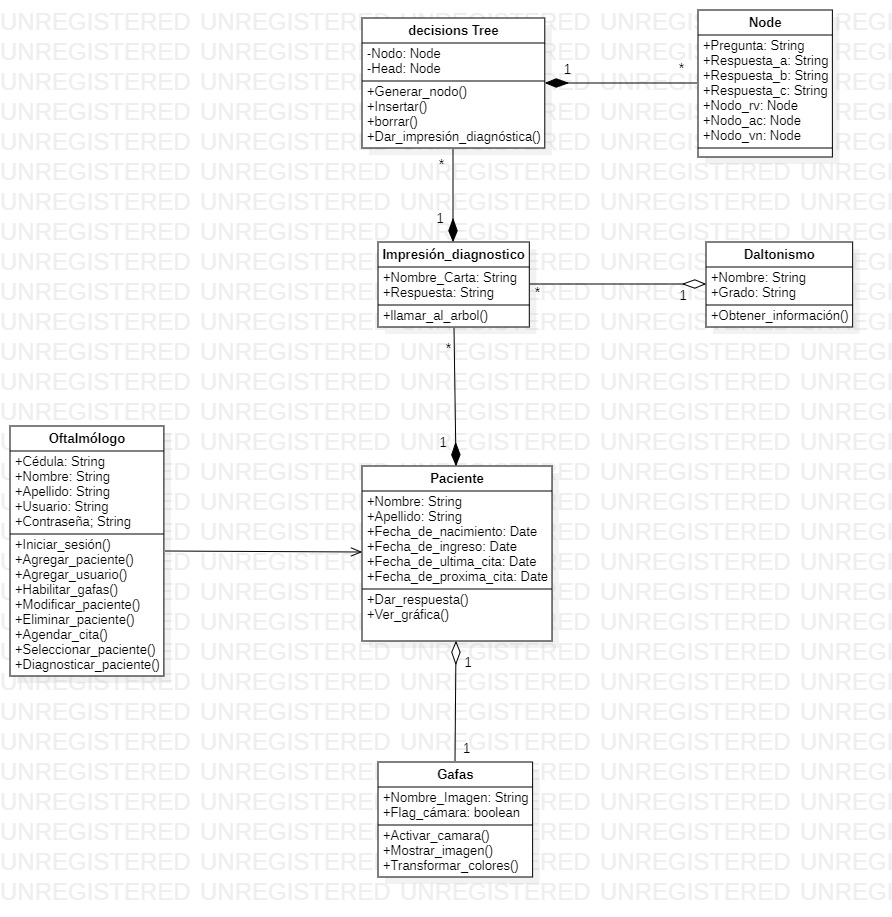
\includegraphics[scale = 0.40]{UML/ClassDiagram1.jpg}
\captionof{figure}{\label{fig:2} Diagrama de clases}
	\end{center} 
\end{figure}


\newpage
\subsubsection{Diagrama de de componentes}

Se buscará mostrar todos los componentes que formarán el sistema.

\begin{figure}[H]
	\begin{center}
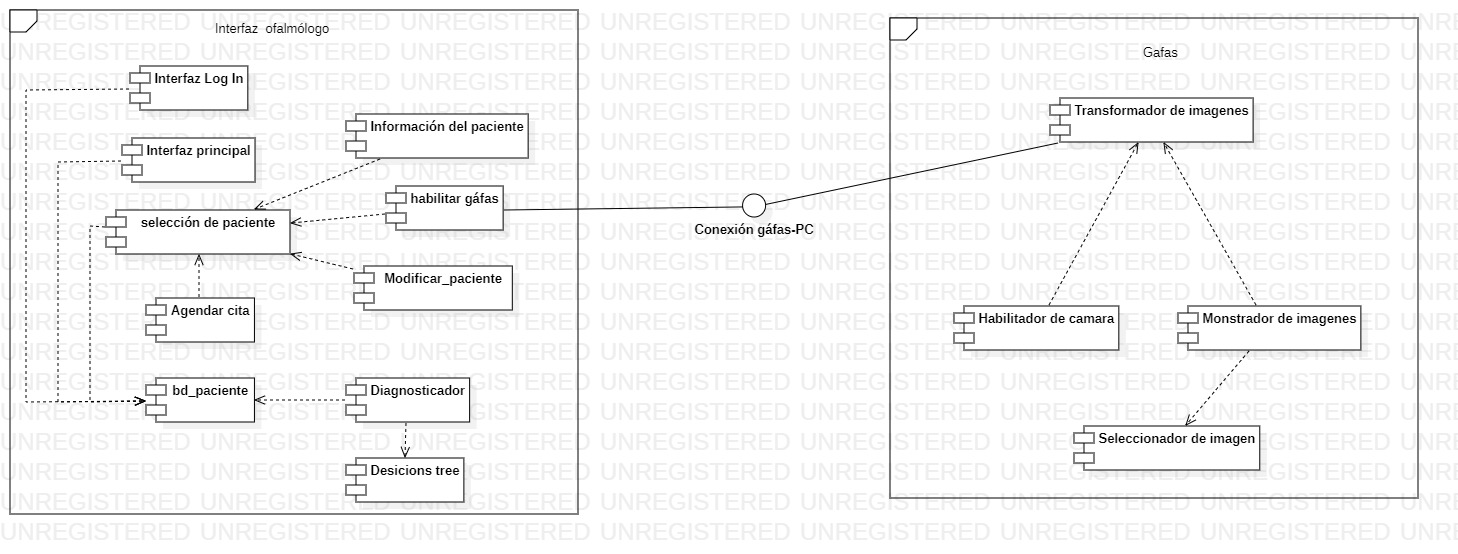
\includegraphics[scale = 0.30]{UML/ComponentDiagram1.jpg}
\captionof{figure}{\label{fig:2} Diagrama de componentes}
	\end{center} 
\end{figure}

\subsubsection{Diagrama de estados}

Este diagrama muestra los estados en el que sistema podría encontrarse.

\begin{figure}[H]
	\begin{center}
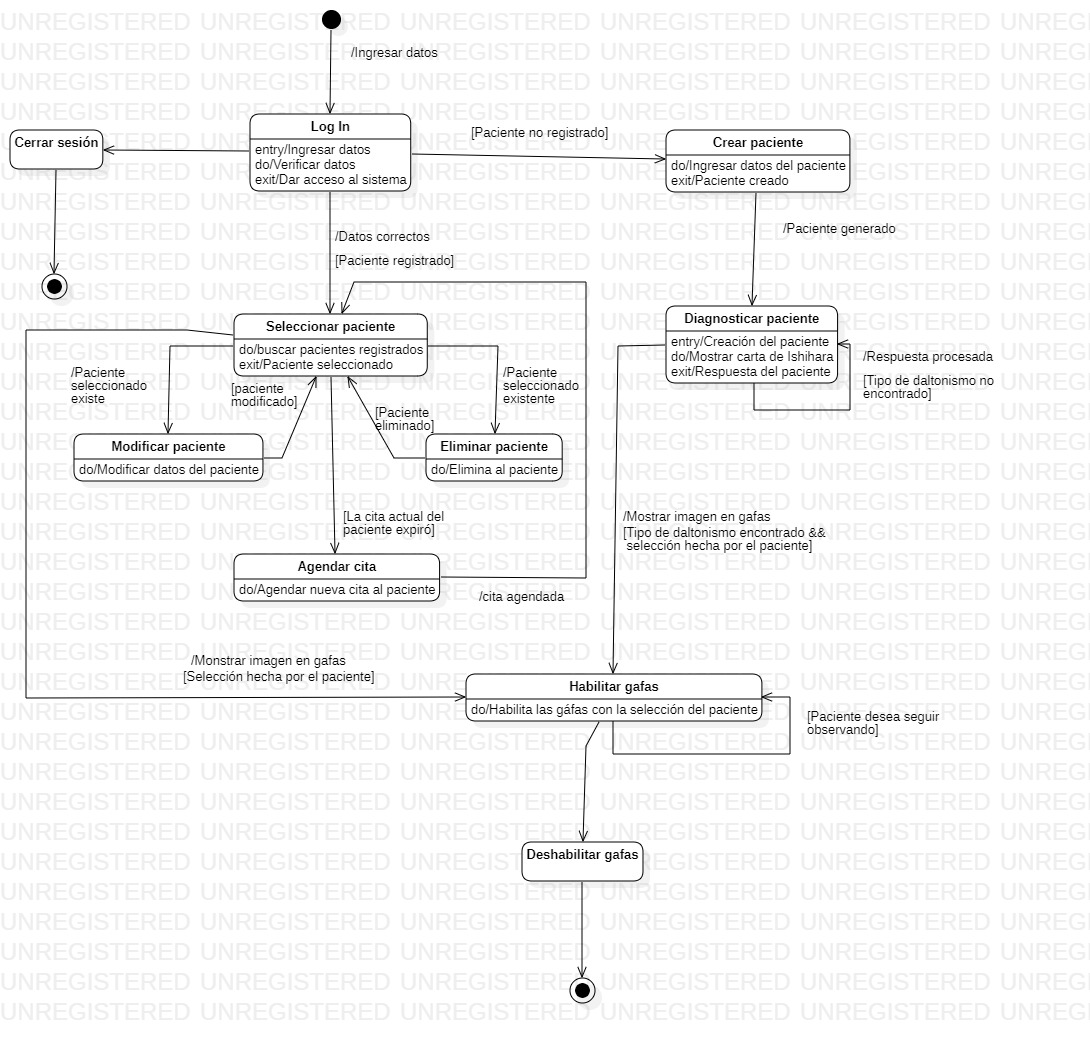
\includegraphics[scale = 0.30]{UML/StatechartDiagram1.jpg}
\captionof{figure}{\label{fig:2} Diagrama de estados}
	\end{center} 
\end{figure}
\newpage
\subsubsection{Diagrama de secuencia}

Estos diagrama coloca a través del tiempo, la secuencia que este tendrá cada caso de uso.

\begin{figure}[H]
	\begin{center}
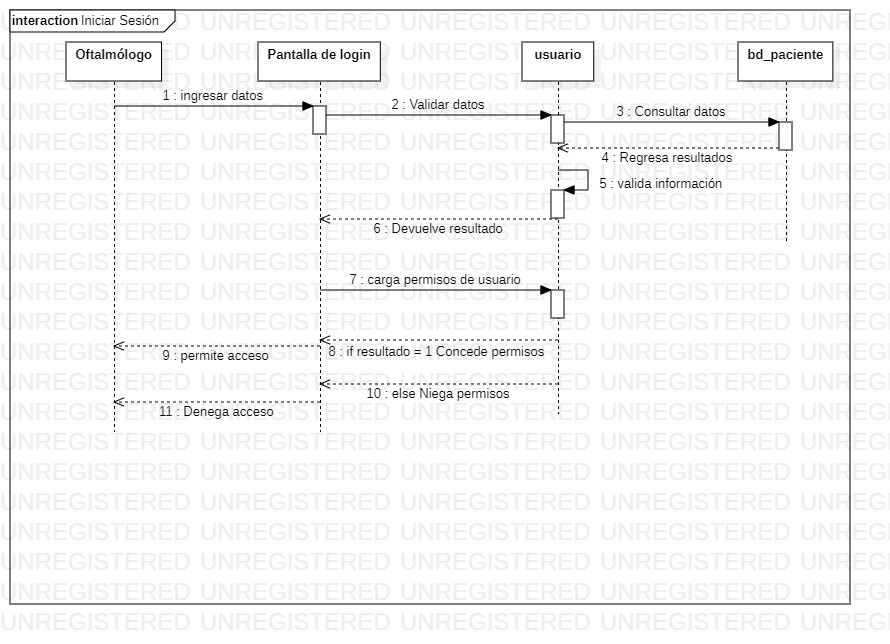
\includegraphics[scale = 0.45]{UML/Secuencias/Caso_de_uso_1.jpg} 
\captionof{figure}{\label{fig:2} Diagrama de secuencia}
	\end{center} 
\end{figure}

\begin{figure}[H]
	\begin{center}
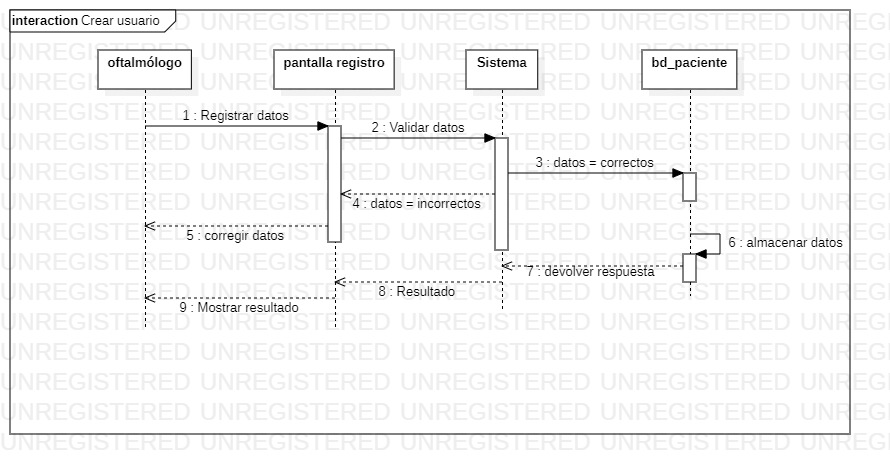
\includegraphics[scale = 0.45]{UML/Secuencias/Caso_de_uso_2.jpg} 
\captionof{figure}{\label{fig:2} Diagrama de secuencia}
	\end{center} 
\end{figure}


\begin{figure}[H]
	\begin{center}
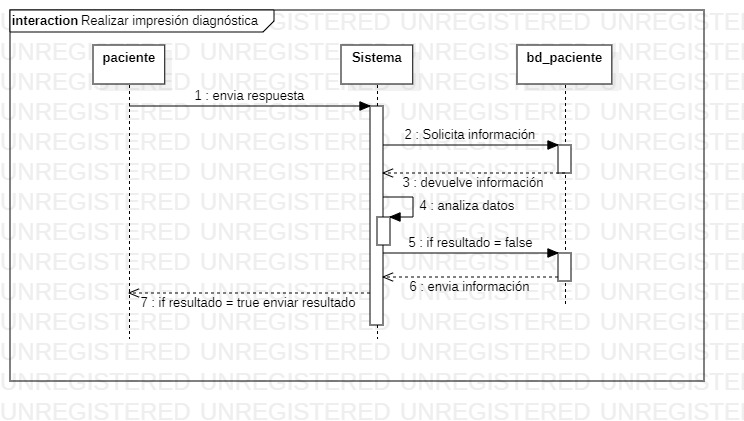
\includegraphics[scale = 0.45]{UML/Secuencias/Caso_de_uso_3.jpg} 
\captionof{figure}{\label{fig:2} Diagrama de secuencia}
	\end{center} 
\end{figure}


\begin{figure}[H]
	\begin{center}
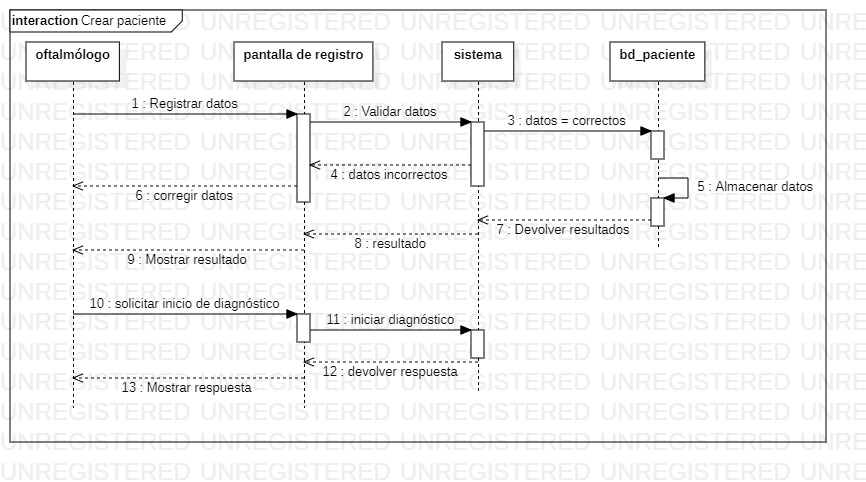
\includegraphics[scale = 0.45]{UML/Secuencias/Caso_de_uso_4.jpg} 
\captionof{figure}{\label{fig:2} Diagrama de secuencia}
	\end{center} 
\end{figure}


\begin{figure}[H]
	\begin{center}
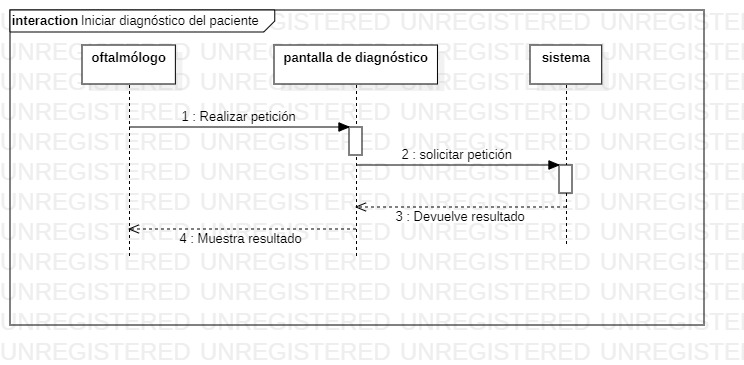
\includegraphics[scale = 0.45]{UML/Secuencias/Caso_de_uso_5.jpg} 
\captionof{figure}{\label{fig:2} Diagrama de secuencia}
	\end{center} 
\end{figure}


\begin{figure}[H]
	\begin{center}
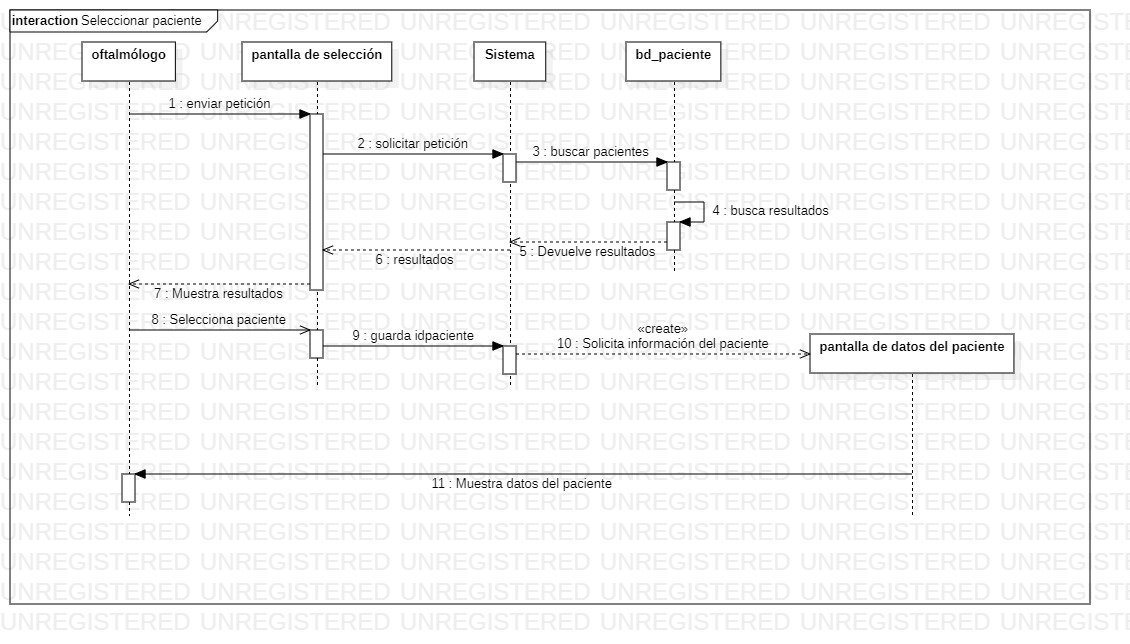
\includegraphics[scale = 0.40]{UML/Secuencias/Caso_de_uso_6.jpg} 
\captionof{figure}{\label{fig:2} Diagrama de secuencia}
	\end{center} 
\end{figure}


\begin{figure}[H]
	\begin{center}
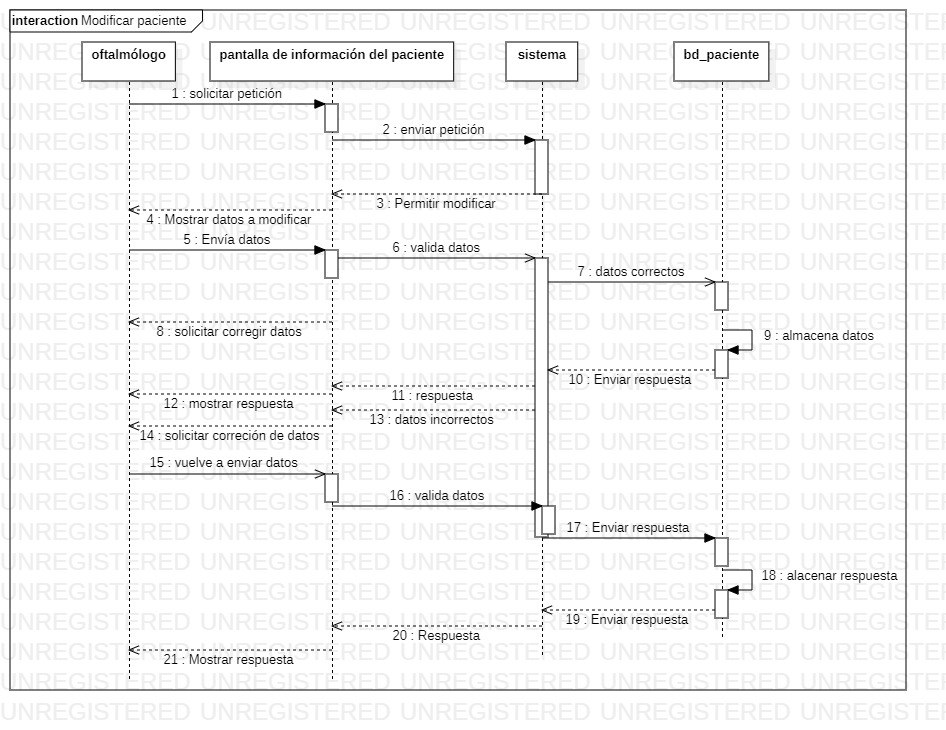
\includegraphics[scale = 0.45]{UML/Secuencias/Caso_de_uso_7.jpg} 
\captionof{figure}{\label{fig:2} Diagrama de secuencia}
	\end{center} 
\end{figure}


\begin{figure}[H]
	\begin{center}
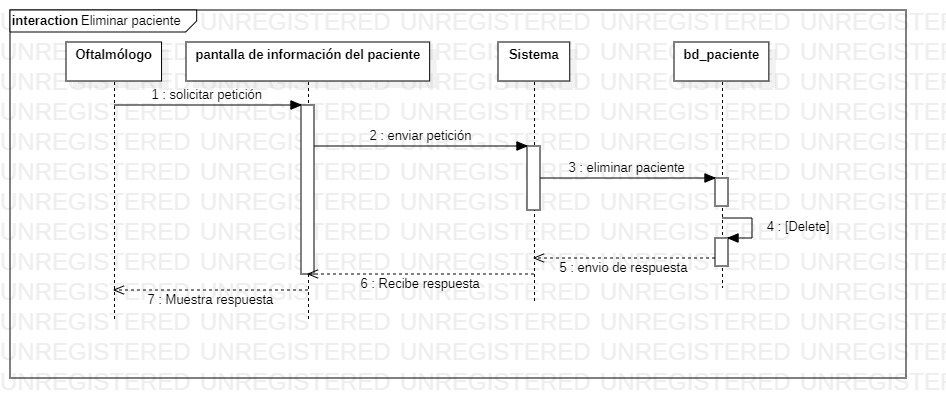
\includegraphics[scale = 0.45]{UML/Secuencias/Caso_de_uso_8.jpg} 
\captionof{figure}{\label{fig:2} Diagrama de secuencia}
	\end{center} 
\end{figure}


\begin{figure}[H]
	\begin{center}
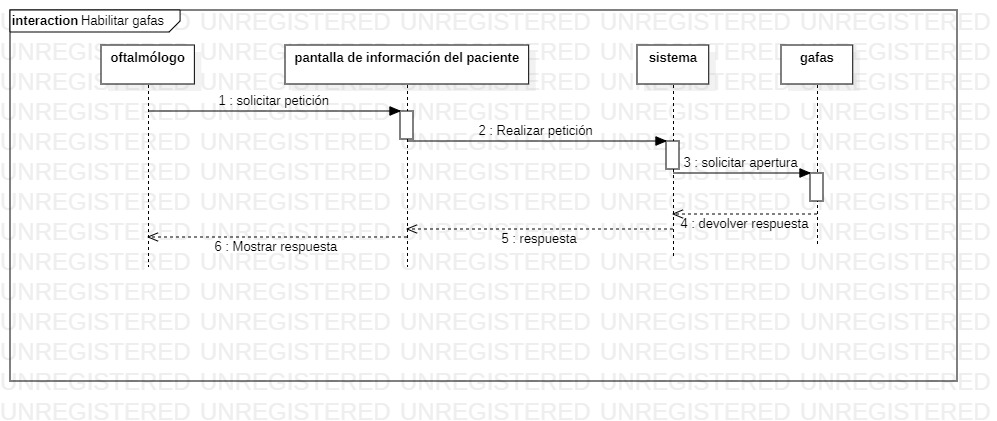
\includegraphics[scale = 0.45]{UML/Secuencias/Caso_de_uso_9.jpg} 
\captionof{figure}{\label{fig:2} Diagrama de secuencia}
	\end{center} 
\end{figure}


\begin{figure}[H]
	\begin{center}
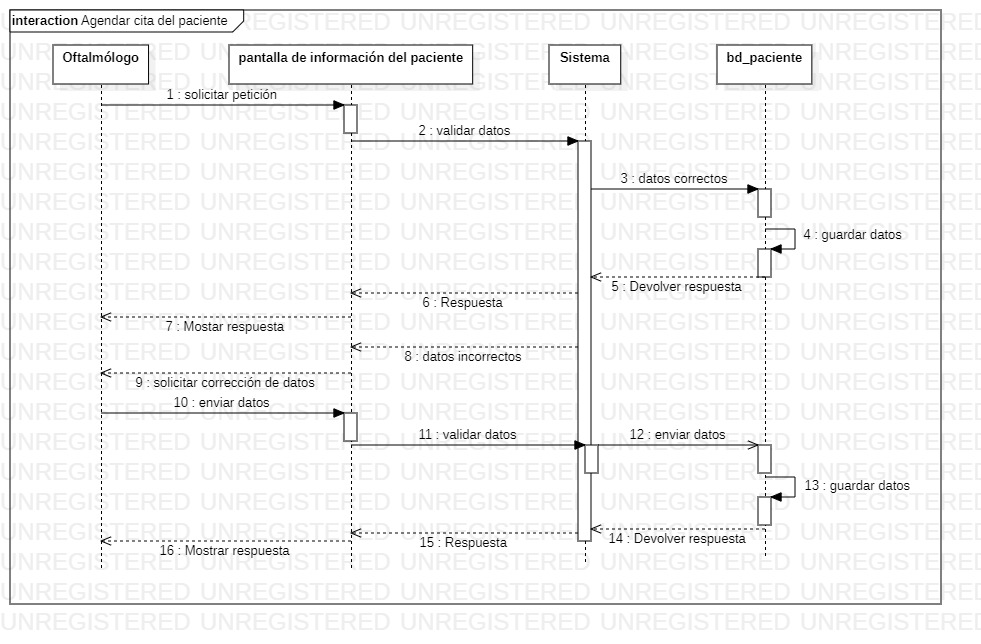
\includegraphics[scale = 0.45]{UML/Secuencias/Caso_de_uso_10.jpg} 
\captionof{figure}{\label{fig:2} Diagrama de secuencia}
	\end{center} 
\end{figure}


\begin{figure}[H]
	\begin{center}
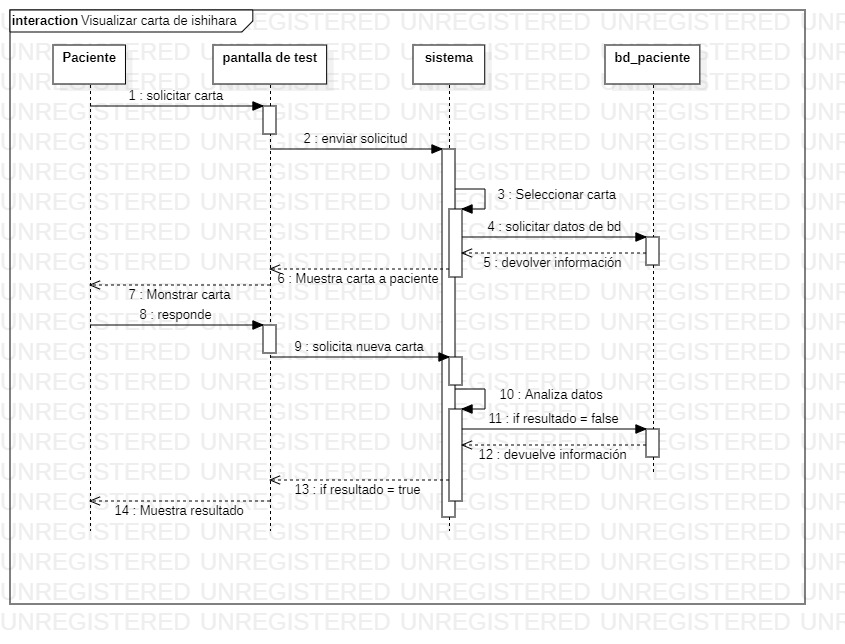
\includegraphics[scale = 0.45]{UML/Secuencias/Caso_de_uso_11.jpg} 
\captionof{figure}{\label{fig:2} Diagrama de secuencia}
	\end{center} 
\end{figure}

\newpage

\subsubsection{Diagrama de actividades}

Este diagrama muestra todas las actividades que realizará el sistema.

\begin{figure}[H]
	\begin{center}
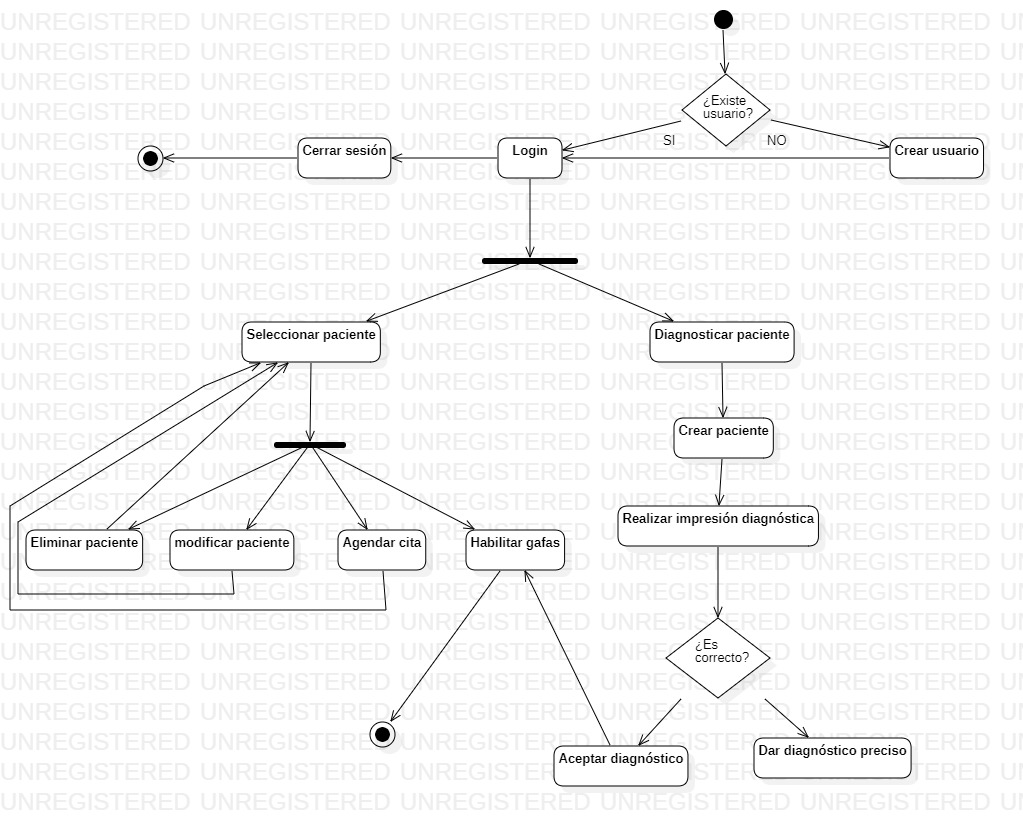
\includegraphics[scale = 0.45]{UML/ActivityDiagram1.jpg}
\captionof{figure}{\label{fig:2} Diagrama de actividades}
	\end{center} 
\end{figure}

\newpage

\subsection{Diagrama Entidad-Relación}

Como se debe incluir una Base de datos que almacene los doctores y los pacientes, se debe incluir de igual manera un diagrama Entidad-relación.

\begin{figure}[H]
	\begin{center}
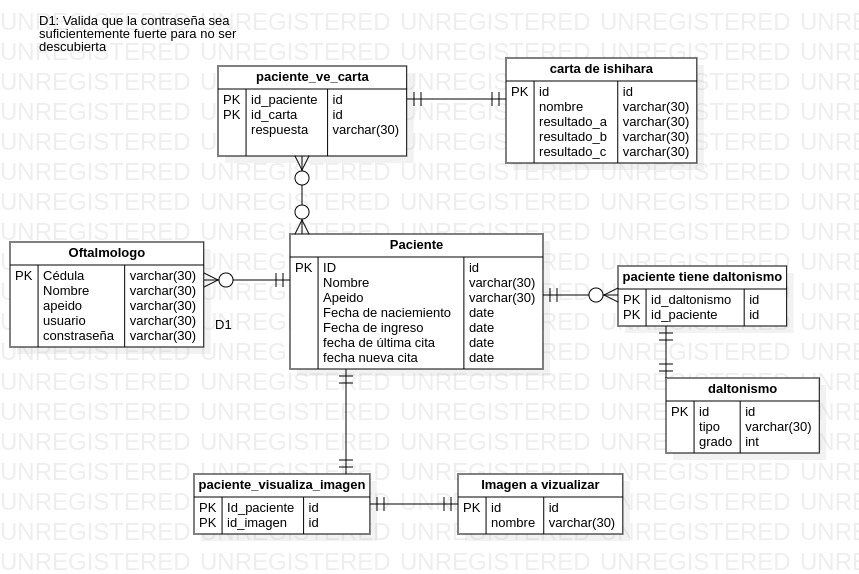
\includegraphics[scale = 0.50]{UML/ERDDiagram1.jpg}
\captionof{figure}{\label{fig:2} Diagrama entidad relación}
	\end{center} 
\end{figure}

\newpage

\subsection{Diagrama de Flujo}

El diagrama de flujo trata de mostrar el flujo que llevará a través del tiempo el sistema y los diferentes procesos en los que puede estar la herramienta presente.

\begin{figure}[H]
	\begin{center}
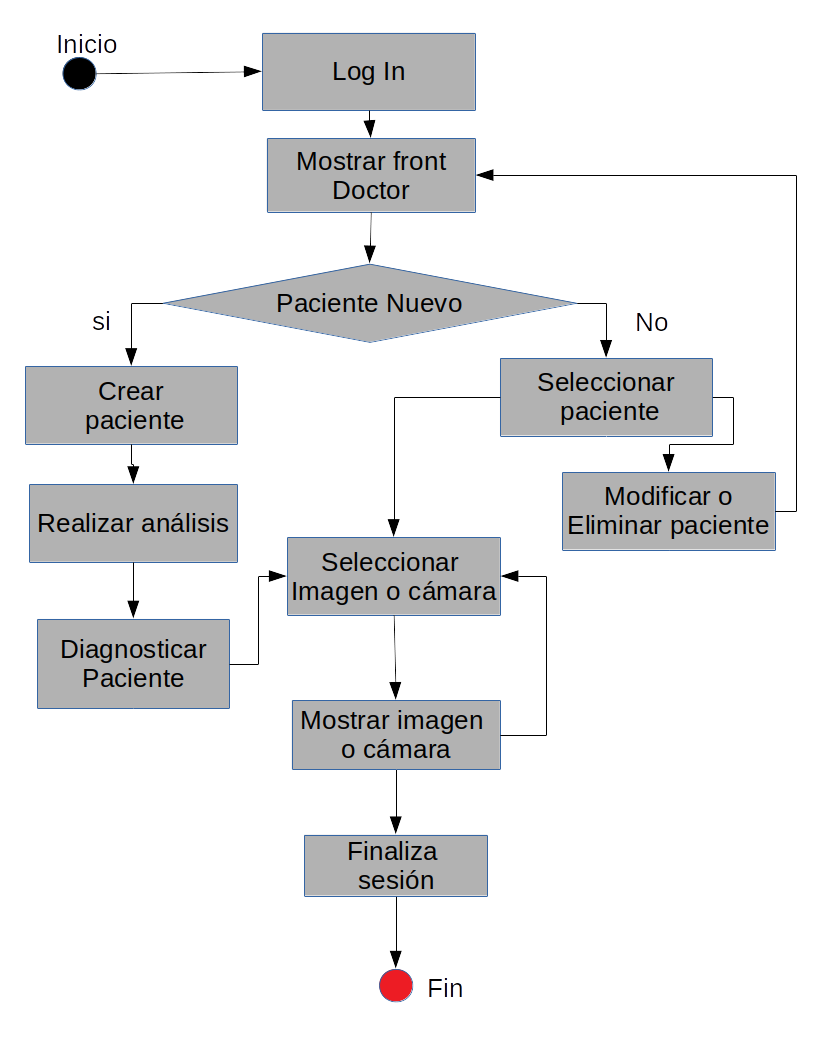
\includegraphics[scale = 0.70]{Imagenes/flow.png}
\captionof{figure}{\label{fig:2} Diagrama de flujo}
	\end{center} 
\end{figure}

\subsection{maquetado}
Las siguientes serán plantillas de las posibles pantallas finales que podrá observar el usuario, primeramente mostraremos las que observará el paciente y posteriormente las mostradas al oftalmólogo.
\subsubsection{Ventanas del paciente}

\begin{figure}[H]
	\begin{center}
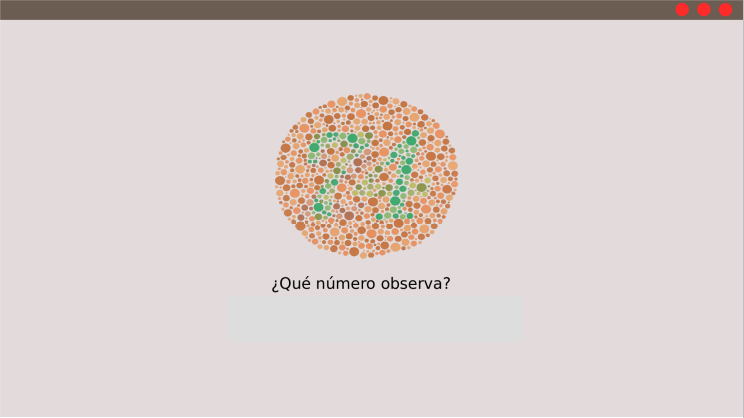
\includegraphics[scale = 0.50]{Imagenes/Ventana5.png}
\captionof{figure}{\label{fig:2} Ventana con carta de ishihara}
	\end{center} 
\end{figure}

\subsubsection{Ventanas del olftalmólogo}


\begin{figure}[H]
	\begin{center}
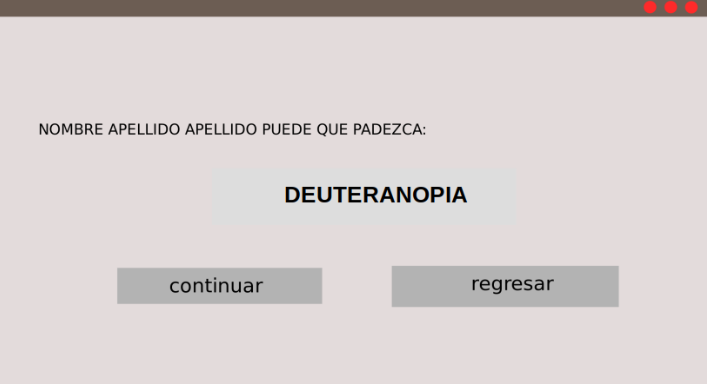
\includegraphics[scale = 0.60]{Imagenes/Ventana6.png}
\captionof{figure}{\label{fig:2} Resultado }
	\end{center} 
\end{figure}

\begin{figure}[H]
	\begin{center}
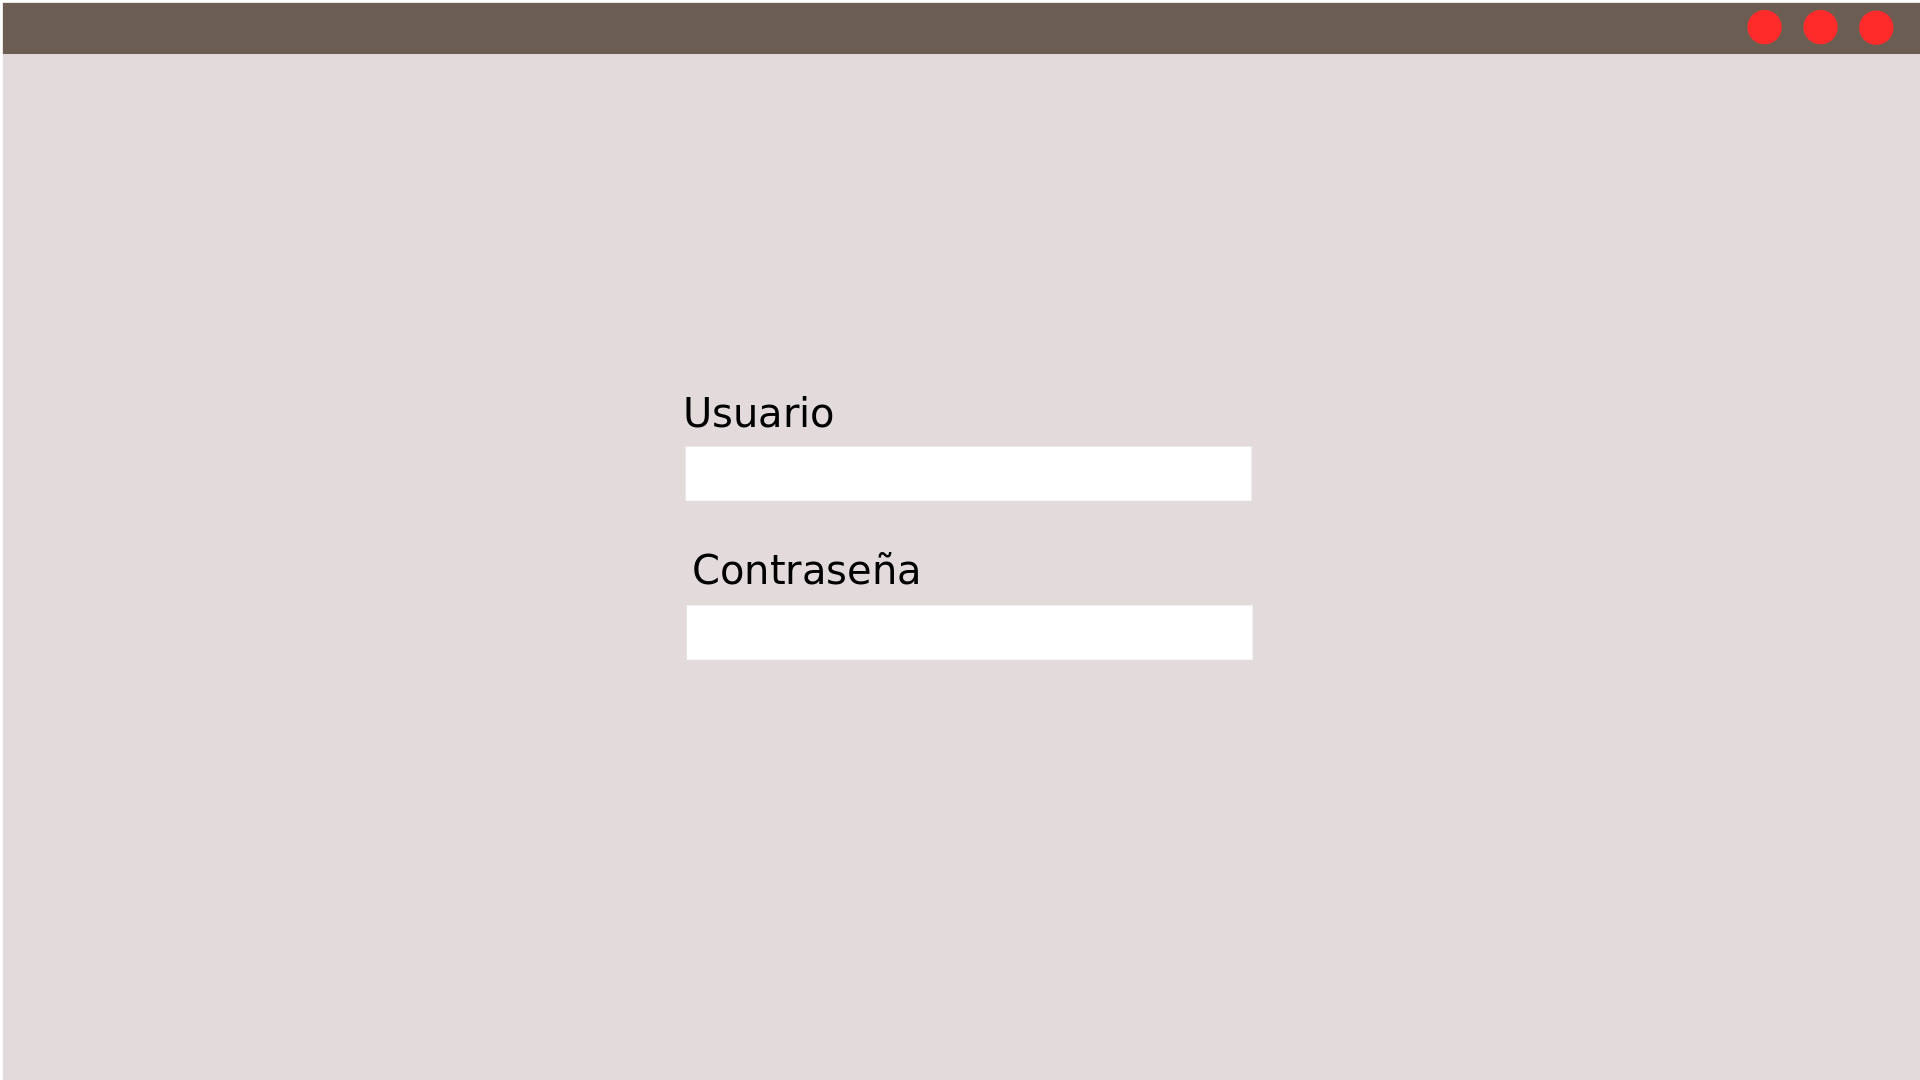
\includegraphics[scale = 0.20]{Imagenes/login.png}
\captionof{figure}{\label{fig:2} LogIn del oftalmólogo}
	\end{center} 
\end{figure}

\begin{figure}[H]
	\begin{center}
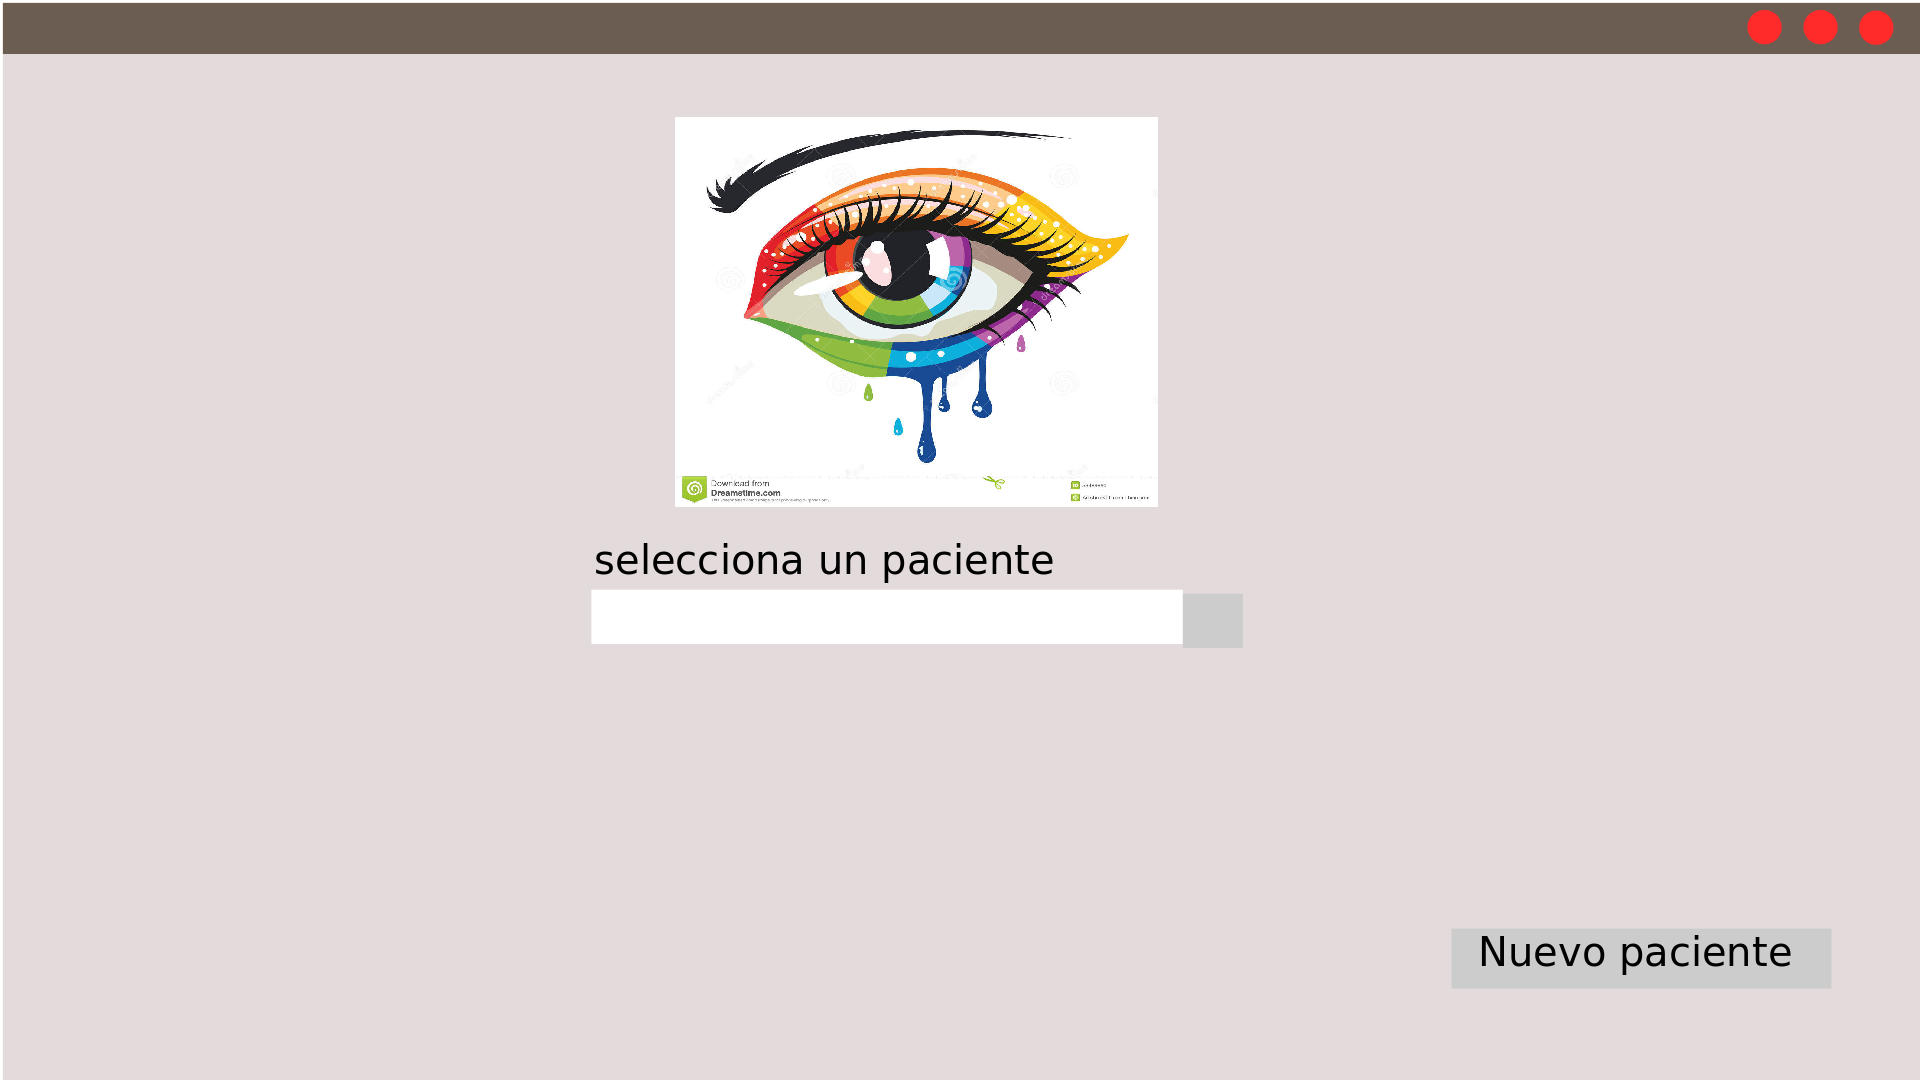
\includegraphics[scale = 0.20]{Imagenes/Ventana2.png}
\captionof{figure}{\label{fig:2} Ventana con carta de selección de un paciente}
	\end{center} 
\end{figure}
\newpage


\begin{figure}[H]
	\begin{center}
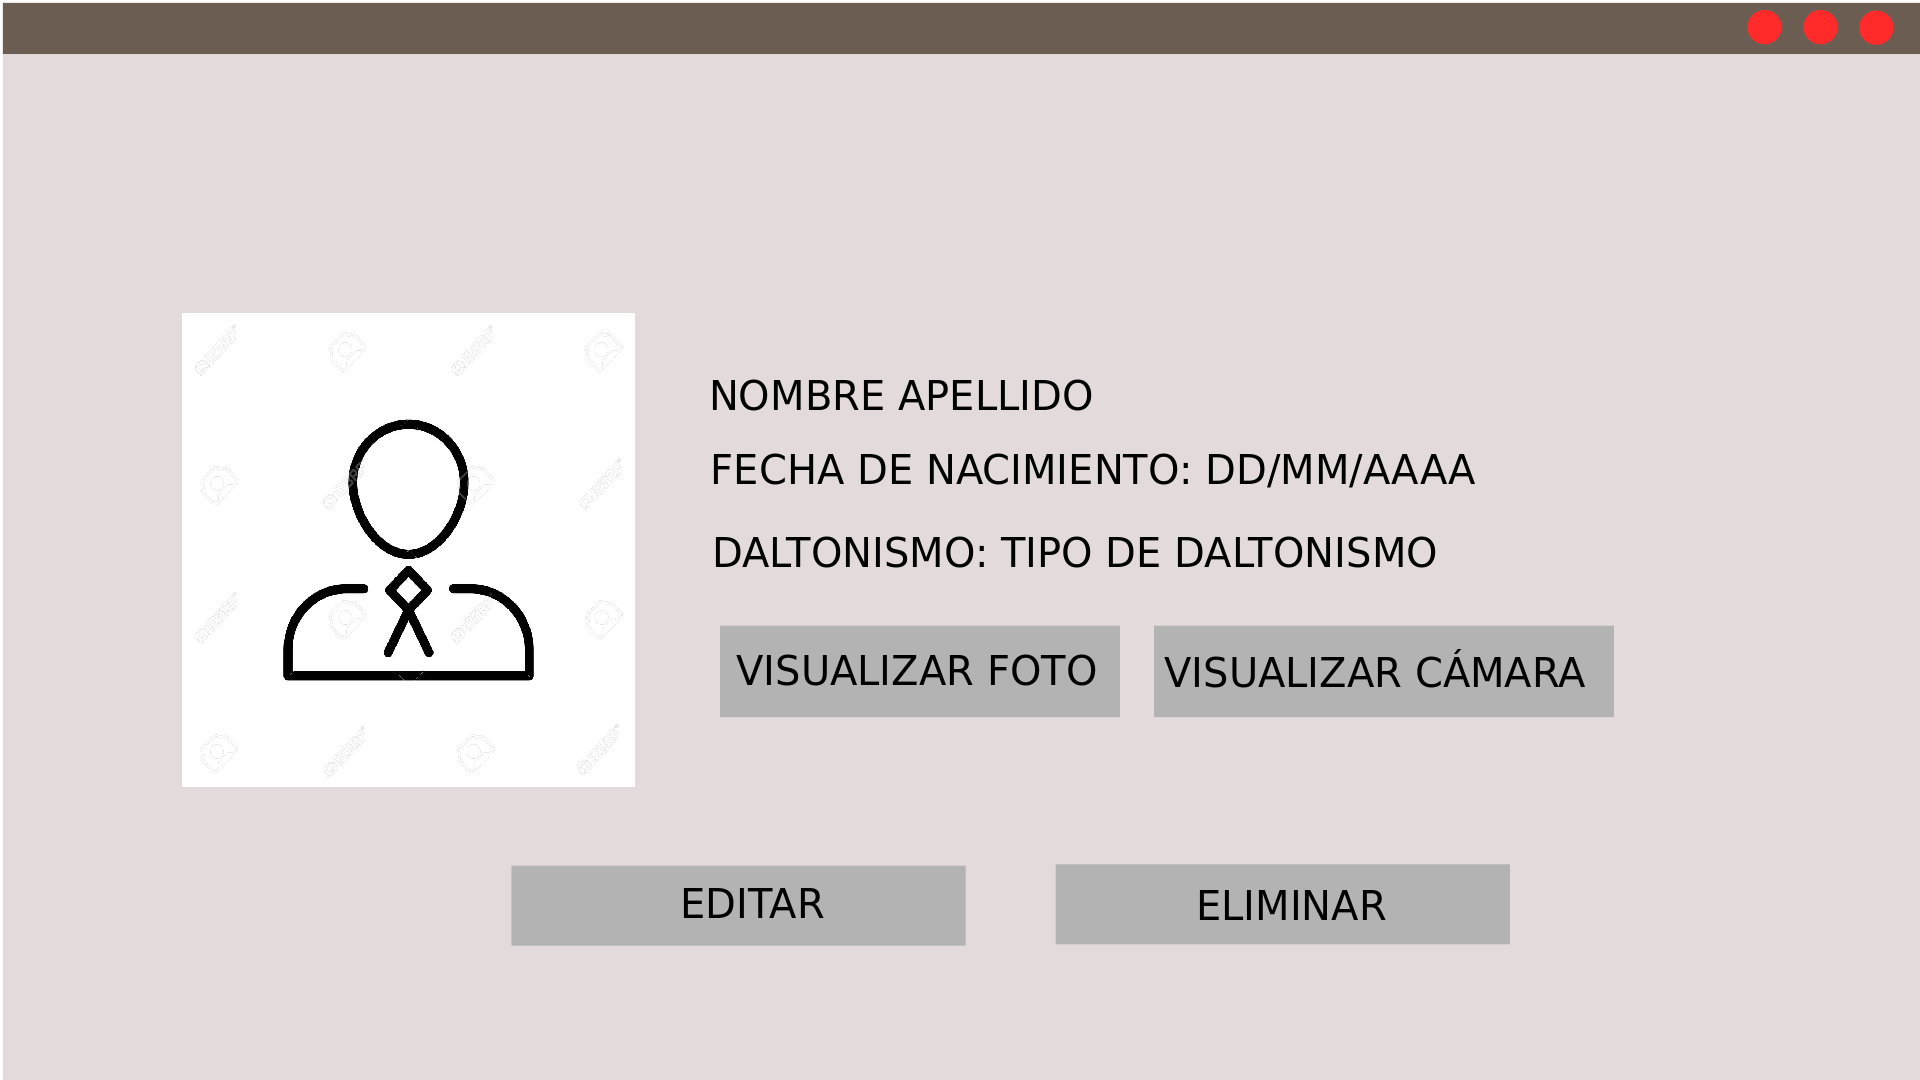
\includegraphics[scale = 0.20]{Imagenes/Ventana3.png}
\captionof{figure}{\label{fig:2} Ventana con información del paciente}
	\end{center} 
\end{figure}


\begin{figure}[H]
	\begin{center}
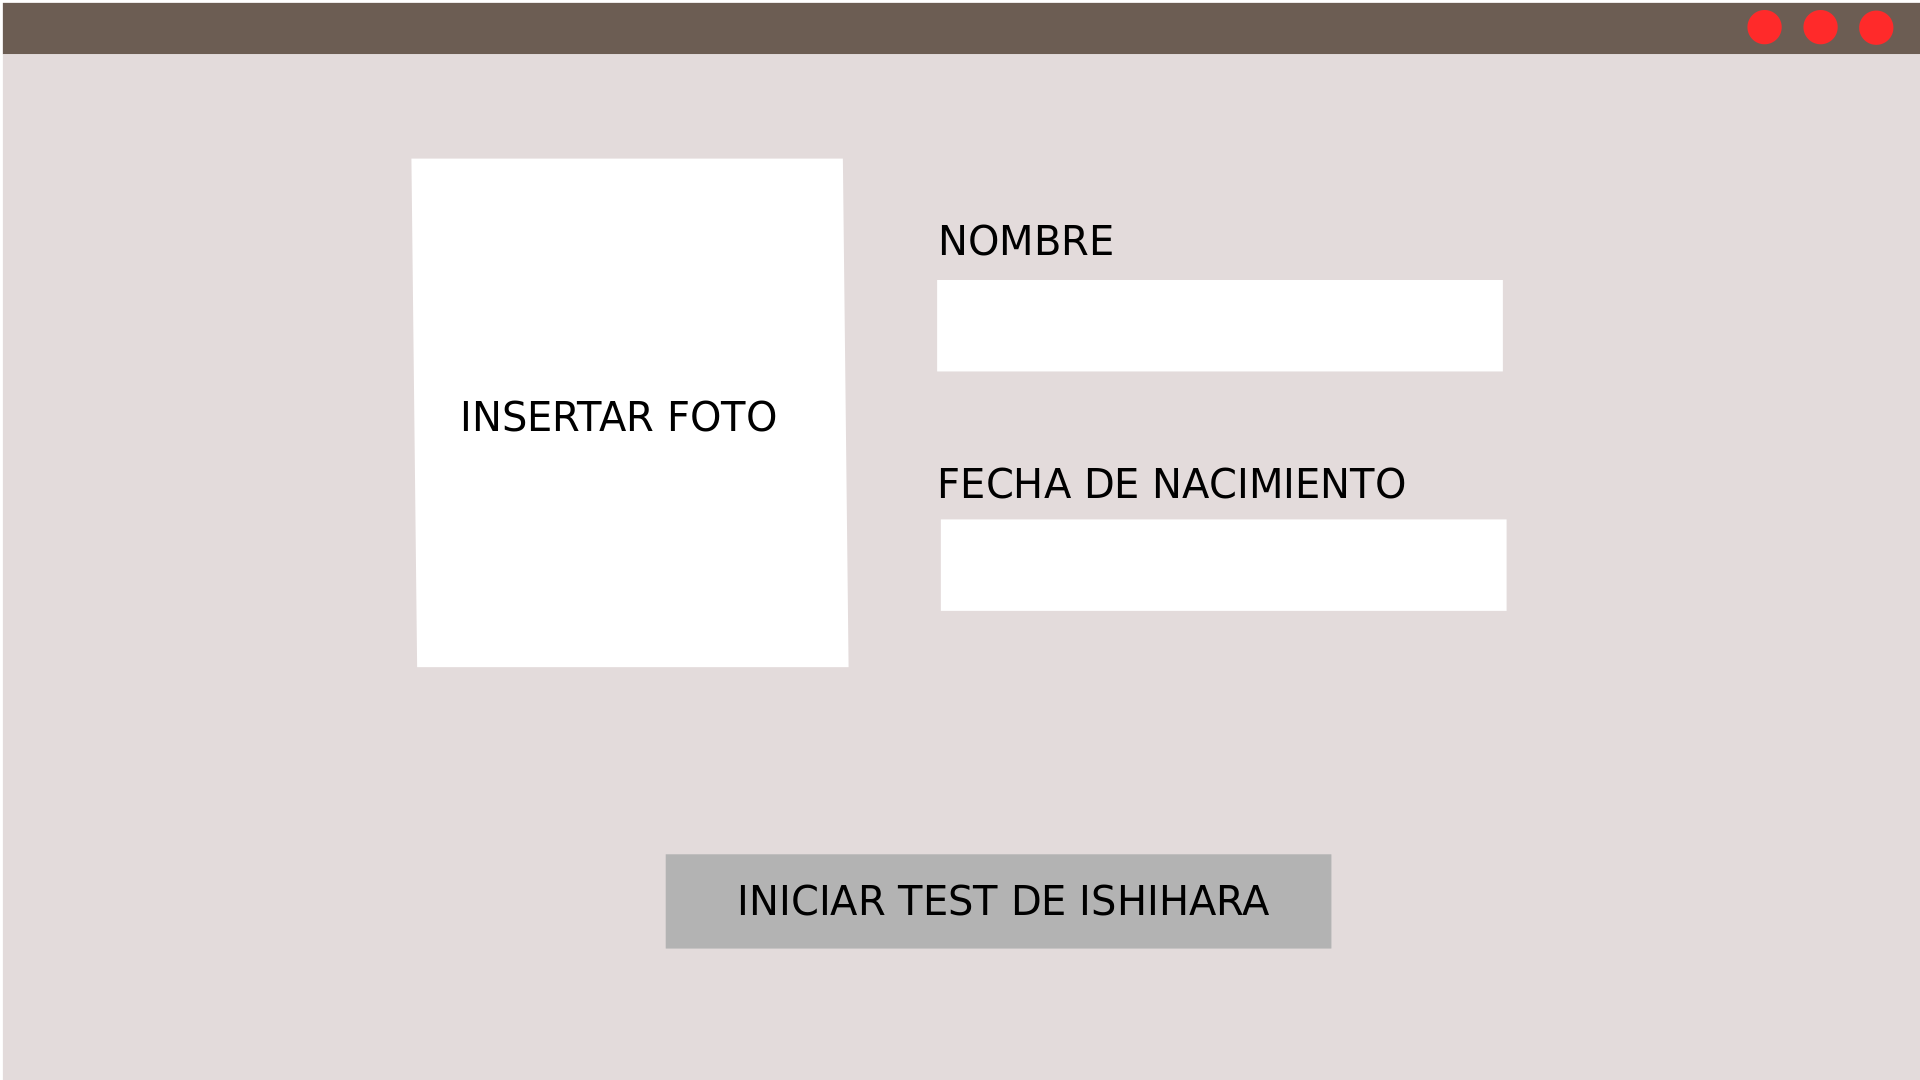
\includegraphics[scale = 0.20]{Imagenes/Ventana4.png}
\captionof{figure}{\label{fig:2} Ventana de insersión de datos del nuevo paciente}
	\end{center} 
\end{figure}

\newpage
\section{Construcción}

\subsection{Construcción de Módulo de \textit{Log In}}

Como se había planteado en el \textit{Log In} del sistema, se ocupó Java, especificamente \textbf{Java JDK 8.221} junto con el conector de \textbf{JDBC 5.1.48} y el \textbf{mysql 8.0.19}, con los que a través de \textbf{Neatbeans 8.2} realizamos las interfaces gráficas que facilitan el como se verán cada uno de los \textit{front-end} que serán visibles para el oftalmólogo, en el caso especial de java se ocupan para introducir los datos, dos \textit{JOptionPane.InputMessage}, los cuales guardarán en datos de tipo \textit{String} las cadenas que serán introducidas en el \textit{Query} que será enviado a la base de datos, la cual regresará un 1 en caso de ser exitoso y 0 en el caso contrario, facilitándonos el saber si este se encuentra dentro la base de datos.

\subsection{Construcción de la base de datos bd\_paciente}

La base de datos, como ya se mencionó con anterioridad se construyó con \textbf{mysql 8.2}, basándose y conservando el diseño que se realizó en el diagrama de entidad relación, esto incluye llaves primarias y foráneas, tipos de datos y si estos reciben un autoincremento o no pueden ser nulos.

El llenado de los usuarios, al haber tenido la prueba realizada con anterioridad con pacientes reales a través de un \textit{Google Forms} y diagnósticos con pacientes presenciales, fue primeramente manual, discerniendo a pacientes daltónicos encontrados.


\newpage
\section{Conclusiones.}

El daltonismo es una alteración poco atendida, y si bien un sistema no puede ser la cura para este tipo de alteración, si puede ser una herramienta para brindarle a quien la padece, una mejor calidad de vida e inclusive brindarle un apoyo desde una etapa temprana para que él o la paciente que lo padece pueda saber y conocer más a fondo sobre este padecimiento.

Los sistemas apoyarán en cada momento al Oftalmólogo a que pueda diagnosticar de manera más eficiente, fácil y sencilla, si el paciente padece algún tipo de daltonismo.

Recordemos que el daltonismo es una alteración que no puede ser detectada por uno mismo y que aunque a la mayoria de la población le parece indiferente tiende a ser un problema que es más común de lo que parece, de igual manera, afectando más de lo que se considera, encontrando casos muy particulares en diferentes ámbitos del entretenimiento y la ciencia.

Un algoritmo básico de la \textit{Machine Learning} como lo son los árboles de decisión nos pueden apoyar a clasificar de manera correcta el tipo de daltonismo que padece la persona.

Gracias al alto uso de los colores de la gama cromática RGB, podemos transformar y colocar ciertos filtros a los colores que nos permiten asemejar el correcto espectro de colores que una persona con algún tipo de daltonismo no puede visualizar.

Un problema sigue siendo la acromatopsia, debido a que a que la persona carece de conos o en su defecto son defectuosos, provocando que no se pueda visualizar algún color, por lo que no hay manera de recrear algún tipo de color en el espectro que el visualiza, por lo que se vuelve una tarea imposible, el mostrarle la gama correcta del espectro de colores.

Para finalizar me gustaría puntuar que esta herramienta es un gran avance para el apoyo a este tipo de gente y podría ser la apertura a más investigación sobre el tema y en un futuro conocer más sobre la alteración, siendo los sistemas una ayuda fundamental para que la gente con este tipo de ceguera se integren y no sea una limitante laboral, educacional, médica o social.
\newpage
\section{Glosario}

\begin{enumerate}
\item \textbf{Ojo:} Es el órgano que permite recrear una imagen del exterior, transformando la luz en pequeños impulsos eléctricos, los cuales viajan a través de billones de neuronas, además del nervio óptico, conectados a la corteza visual, en donde se analiza la información y se intenta identificar lo que se está viendo \cite{IEEEreferencias:Ref34}. 
\item \textbf{Nervio óptico:} Un conjunto de fibras nerviosas que conectan la retina con el cerebro. El nervio óptico lleva las señales de luz, oscuridad y los colores al área del cerebro (la corteza visual) que convierte dichas señales en imágenes (por ejemplo, nuestra visión) \cite{IEEEreferencias:Ref35}.
Pupila. La abertura en el centro del iris a través del cual la luz pasa a la parte posterior del ojo \cite{IEEEreferencias:Ref35}. 
\item \textbf{Retina:} La capa nerviosa sensible a la luz que recubre la parte posterior del ojo, capta la luz y crea impulsos que son enviados a través del nervio óptico al cerebro. Y cuenta con dos fotorreceptores conos y bastones \cite{IEEEreferencias:Ref35}. 
iris.\textbf{La parte coloreada del ojo:} El iris es parcialmente responsable de regular la cantidad de luz que ingresa al ojo \cite{IEEEreferencias:Ref35}. 
\item \textbf{Lente (cristalino):} La estructura transparente dentro del ojo que enfoca los rayos de luz en la retina \cite{IEEEreferencias:Ref35}. 
\item \textbf{El núcleo geniculado lateral (NGL):} es un núcleo talámico estructurado histológicamente en capas, comunicadas entre sí, reciben aferencias procedentes de la retina \cite{IEEEreferencias:Ref36}. 
\item \textbf{Córtex visual:} parte de la corteza principalmente dedicada al procesamiento de la estimulación visual proveniente de los fotorreceptores de la retina. Se trata de uno de los sentidos más representados a nivel de corteza, ocupando su procesamiento la mayor parte del lóbulo occipital y una pequeña parte de los parietales \cite{IEEEreferencias:Ref37}. 
\item \textbf{Daltonismo:} está enmarcado en la discromatopsia, un término que hace referencia a un inconveniente basado en la incapacidad para diferenciar los colores \cite{IEEEreferencias:Ref1}. 
\item \textbf{Cornea:} es una estructura del ojo que permite el paso de la luz desde el exterior al interior del ojo y protege el iris y el cristalino. Posee propiedades ópticas de refracción y para garantizar su función debe ser transparente y es necesario que mantenga una curvatura adecuada. La córnea está integrada por seis capas celulares: el epitelio corneal, la membrana de Bowman, el estroma corneal, la capa de DUA, la membrana de Desemet y el epitelio posterior o endotelio corneal \cite{IEEEreferencias:Ref6}.
\item \textbf{Rodopsina:} Compuesto pigmentado de color violáceo que hay en los bastoncillos de la retina. Está formado por una proteína y un derivado de la vitamina A (la opsina y el retinal, respectivamente). Su función es permitir la visión en entornos con poca intensidad de luz \cite{IEEEreferencias:Ref38}.
\item \textbf{Opsina:} Proteína que forma parte del pigmento visual rodopsina junto con cisretineno. Bajo la acción de la luz la rodopsina se descompone en estos dos componentes \cite{IEEEreferencias:Ref39}.
\item \textbf{Maculopatia:} Degeneración macular que afecta principalmente a la mácula lútea de la retina \cite{IEEEreferencias:Ref38}.
\item \textbf{Retinopatia:} Enfermedad ocular de tipo no inflamatorio causada por una alteración de los vasos sanguíneos retinianos \cite{IEEEreferencias:Ref38}.
\item \textbf{Glaucoma:} Degradación del nervio óptico. Esta enfermedad ocular suele estar causada por un exceso de presión intraocular. Si no se trata puede llegar a dañar el nervio óptico irreversiblemente, provocando ceguera. La presión normal del ojo es de 12 a 21 mmHg \cite{IEEEreferencias:Ref38}.
\item \textbf{Gunilato ciclasa:} Enzima que cataliza la ciclación intramolecular del GTP a GMP cíclico liberando PPi \cite{IEEEreferencias:Ref39}.
\item  \textbf{Guanosin trifosfato:} un nucleótido compuesto por ribosa, guanina y un grupo trifosfato. Tiene, al igual que otros nucleósidos trifosfato, una función energética en el metabolismo celular \cite{IEEEreferencias:Ref39}.

\end{enumerate}
\newpage
%%%%%%% Bibliografía %%%%%%%%
\bibliographystyle{bst/IEEEtran.bst} 
\addcontentsline{toc}{section}{Referencias}  
\bibliography{bib/IEEEabrv,bib/IEEEreferencias.bib} 
%%%%%%% Bibliografía %%%%%%%%    

\appendix  
\clearpage % o \cleardoublepage
\addappheadtotoc 
\appendixpage 

\section{Anexo 1}
\newpage
\section{Anexo 2}
\newpage
\section{Anexo 3}
\end{document}